\documentclass[11pt]{amsart} 
\usepackage{amsmath} %Never write a paper without using amsmath for its many new commands 
\usepackage{amssymb} %Some extra symbols 
\usepackage{amsmath}
\usepackage{amsthm}
\usepackage{amssymb}
\usepackage{mathrsfs}
\usepackage[margin=1in]{geometry}
\usepackage{geometry}
\usepackage{graphicx}
\usepackage{fancyhdr}
\usepackage{setspace}
\usepackage{Tabbing}
\usepackage{fancyhdr}
\usepackage{lastpage}
\usepackage{extramarks}
\usepackage{chngpage}
\usepackage{soul,color}
\usepackage{graphicx,float,wrapfig}
\usepackage{enumerate}
\usepackage{mathtools}
\usepackage{multicol}
\usepackage{hyperref}
\usepackage{relsize}
\usepackage{glossaries}
\usepackage[utf8x]{inputenc}
\usepackage{selinput}
\SelectInputMappings{%
  adieresis={ä},
  eacute={é},
  Lcaron={Ľ},
}

\graphicspath{ {/desktop/book} }


 \makeatletter
          \def\@setcopyright{}
          \def\serieslogo@{}
          \makeatother
          \pagestyle{plain}


\cfoot{\thepage}

\advance\footskip0.5cm
\textheight=54pc    %a4paper
%\textheight=50.5pc %letterpaper
\advance\textheight-0.4cm
\calclayout

\setlength{\topmargin}{0in}
\setlength{\oddsidemargin}{0in}

\setlength{\evensidemargin}{0in}

\setlength{\headheight}{0in}

\setlength{\headsep}{0in}


\setlength{\textheight}{9in}

\setlength{\textwidth}{6.5in}

\setlength{\parindent}{0cm}

\setlength{\parskip}{0cm}


\linespread{1.9}

\setlength{\parindent}{0cm} \setlength{\parskip}{0cm}
\author{K. Gray} 
\title{Real Analysis Notebook} 

\raggedbottom

\begin{document} 



 \newcommand{\Q}{{\mathbb Q}}
          \newcommand{\R}{{\mathbb R}}
          \newcommand{\sR}{{\mathcal R}}
          \newcommand{\nil}{\varnothing}
          \newcommand{\N}{{\mathbb N}}
          \newcommand{\A}{{\mathcal A}}
           \newcommand{\E}{{\mathcal E}}
           \newcommand{\M}{{\mathcal M}}
           \newcommand{\Ps}{{\mathcal P}}
           \newcommand{\F}{{\mathcal F}}
           \newcommand{\sa}{{\sigma}\text{-algebra}}
            \newcommand{\B}{{\mathcal B}}
 \newcommand{\SO}{{\mathcal O}}
 \newcommand{\sN}{{\mathcal N}}
 \newcommand{\sL}{{\mathcal L}}
 \newcommand{\C}{{\mathcal C}}
\newcommand{\Z}{{\mathbb Z}}
\newcommand{\sP}{{\mathcal P}}
\newcommand{\U}{{\mathcal U}}



\makeatletter
\def\thm@space@setup{\thm@preskip=0pt
\thm@postskip=0pt}
\makeatother
\newtheoremstyle{newstyle}      
{} %Aboveskip 
{} %Below skip
{\mdseries} %Body font e.g.\mdseries,\bfseries,\scshape,\itshape
{} %Indent
{\bfseries} %Head font e.g.\bfseries,\scshape,\itshape
{.} %Punctuation afer theorem header
{ } %Space after theorem header
{} %Heading

\theoremstyle{newstyle}
\newtheorem{thm}{Theorem}
\newtheorem{prop}{Proposition}
\newtheorem{lem}{Lemma}
\newtheorem{cor}{Corollary}
\newtheorem{dfn}{Definition}
\newtheorem*{construction}{Construction}
\newtheorem*{example}{Example}
\newtheorem*{conjecture}{Conjecture}
\newtheorem{rmk}{Remark}

\makeatletter
\newenvironment{pf}[1][\proofname]{\par
  \pushQED{\qed}%
  \normalfont \topsep0\p@\relax
  \trivlist
  \item[\hskip\labelsep\itshape
  #1\@addpunct{.}]\ignorespaces
}{%
  \popQED\endtrivlist\@endpefalse
}
\makeatother

\maketitle
\thispagestyle{empty}
\pagenumbering{gobble}
\tableofcontents
\cleardoublepage
\pagenumbering{arabic}
\setcounter{page}{1}

\clearpage


\section{Section 1.2 (Folland): $\sigma$-algebras}
\subsection{Section 1.2: Definitions and Theorems}

\begin{dfn}[algebra] An algebra $A$ is a nonempty collection of subsets of a nonempty set $X$ which is closed under finite unions and complements.
\end{dfn}

\begin{example} If $X = \{ 1, 2, 3 \}$ then the following are algebras:
\begin{itemize}
\item $ \{ \emptyset, X \} $,
\item $ \{ \emptyset, \{ 1 \}, \{ 2, 3 \}, X \}$,
\item $ \{ \emptyset, \{ 2 \}, \{ 1, 3 \}, X \} $,
\item $ \{ \emptyset, \{ 3 \}, \{ 1, 2 \}, X \}$, and 
\item $ P(X)$.
\end{itemize}
Any other subset of the power set is not an algebra.
\end{example}

\begin{dfn}[$\sa$] An algebra $A$ is a $\sigma$-algebra if it is closed under countable unions. \end{dfn}

\begin{example}
Any algebra over a finite set is a $\sigma$-algebra, as is the power set of the set $X$. More examples are found in exercises.
\end{example}
\begin{dfn}[co-countable sets] a cocountable subset of a set X is a subset Y whose complement in X is a countable set. In other words, Y contains all but countably many elements of X. While the rational numbers are a countable subset of the reals, for example, the irrational numbers are a cocountable subset of the reals.
\end{dfn}

\begin{dfn}[$\sa$ of co-countable or countable sets] The $\sigma$-algebra of co-countable or countable sets is the collection of subsets such that either the subset or its complement is countable.
\end{dfn}

\begin{prop} Given any nonempty collection $ \mathcal{E}$ in the power set of $X$, there is a smallest $\sigma$-algebra that contains $\mathcal{E}$. 
\begin{proof} The idea of the proof is to show that an arbitrary intersection of $\sigma$-algebras is a $\sigma$-algebra.  One then considers the collection of $\sigma$-algebras that contain $ \mathcal{E}$, which is nonempty since the power set is such a set, and then take the intersection of all such sets.
\end{proof}
\end{prop}
\begin{lem} If a collection of sets $\mathcal{E}$ is contained in a $\sigma$-algebra $\mathcal{B}$ then the $\sigma$-algebra generated by $\mathcal{E}$ is contained in $ \mathcal{B}$. \end{lem}

\begin{dfn}[$\sigma$-algebra generated by $\mathcal{E}$] If $\mathcal{E}$ is a subset of $P(X)$ then the $\sigma$-algebra generated by $\mathcal{E}$ is the smallest $\sigma$-algebra that contains $\mathcal{E}$.
\end{dfn}

\begin{dfn}[Borel $\sigma$-algebra] The Borel $\sigma$-algebra for a metric space $X$ (the $\sigma$-algebra of Borel sets) is the $\sigma$-algebra generated by open sets.
\end{dfn}

\begin{dfn}[$G_{\delta}, F_\sigma$] A set in a metric space is a $G_{\delta}$ set if it is the countable intersection of open sets, it is an $F_{\sigma}$ set if it the countable union of a closed set.
\end{dfn}

\begin{example} $[0,1)$ is an $F_{\sigma}$ set since $ [0,1) = \cup [0, 1- \frac{1}{n}]$.  Any singleton is a $G_{\delta}$ set, it is also an $F_{\sigma}$ set.
\end{example}

\begin{prop} Each of the following sets generates the the Borel sets in $ \mathbb{R}$:
\begin{itemize}
\item open intervals,
\item closed intervals,
\item half open intervals,
\item open rays,
\item closed rays.
\end{itemize} 
\end{prop}

\begin{dfn}[product $\sa$] If $M_{\alpha}$ is a indexed collection of $\sigma$-algebras on an indexed collections of sets $X_{\alpha}$, then the product $\sigma$-algebra on the product space $X = \prod X_{\alpha}$ is the $\sigma$ algebra generated by the inverse image of elements of $M_{\alpha}$ under the coordinate maps $\pi_{\alpha}$.\\
The $\sa$ of subsets of $X \times Y$ generated by the semi-algebra $\sR$ is called the product $\sa$ and is denoted by $\A \otimes \B$.
\end{dfn}

\begin{example}
If $X_1, X_2$ are the indexed set with associated $\sigma$-algebras $M_1, M_2$ then the inverse image of the coordinate maps are sets of the form $ E_1\times X_2$ and $X_1 \times F_2$, where $E_1 \in M_1$ and $F_2 \in M_2$.  Notice that using intersections you get all sets of the form $E_1 \times F_2$.
\end{example}

\begin{prop} The product $\sigma$-algebra (in the case that the index set is countable) is generated by all products of things in the $M_i$'s
\end{prop}

\begin{prop} If each $M_{\alpha}$ is generated by a set $E_{\alpha}$ then the product sigma algebra is generated by elements of the $E_{\alpha}$, rather than arbitrary elements of $M_{\alpha}$. \end{prop}

\begin{thm} If $X_1, X_2, \cdots, X_n$ are metric spaces then the Borel sets on the product space is the product of the Borel sets on the individual spaces.
\end{thm}

\begin{proof}
The proof uses the preceding proposition.
\end{proof}

\begin{dfn}[elementary family] An elementary family is a collection of subsets that contains the empty set, is closed under finite intersections, and the complement of any set in the collection is a finite disjoint union of elements of the collection. \end{dfn}

\begin{example} Any $ \sigma$-algebra is an elementary family. 
In general the point of elementary families is starting with minimal information how does one build a $\sigma$-algebra, vs. knowing that there is a minimal $\sigma$-algebra.\end{example}

\begin{prop} The finite disjoint union of members of an elementary family is an algebra. \end{prop}


\subsection{August 26 Group Assignment}
Note: solutions for the August 26th assignment were provided by Professor Duncan and expanded upon by author.\\
Let $ \{ A_k \}_{k=1}^{\infty}$ be a sequence of sets. We define \[ \limsup_{k \rightarrow \infty} A_k = \bigcap_{j=1}^{\infty} \left( \bigcup_{k=j}^{\infty} A_k \right) \qquad  \text{ and } \qquad  \liminf_{k \rightarrow \infty} A_k = \bigcup_{j=1}^{\infty} \left( \bigcap_{k=j}^{\infty} A_k \right). \]

\begin{enumerate}


\item Prove that $\limsup_{k \rightarrow \infty} A_k = \{ x : x \in A_k \mbox{ for infinitely many } k \}.$
\begin{pf}
	Let $E= \{ x:x \in A_k\ \text{for infinitely many} \ k \}$.  To show $\limsup \limits_{k \rightarrow \infty} A_k =E$, we will show $\limsup \limits_{k \rightarrow \infty} A_k \subseteq E$ and $\limsup \limits_{k \rightarrow \infty} A_k \supseteq E$.
	 First, let's show $\limsup \limits_{k\rightarrow \infty} A_k \subseteq E$. Let $x \in \limsup \limits_{k\rightarrow \infty} A_k$. Suppose for the purposes of contradiction that $x \notin E$. If $x \notin E$, then it is not the case that $x$ is in infinitely many sets $A_k$. If $x$ is not in infinitely many sets $A_k$, then there must exist some $j_0$ such that for all $k\geq j_0$, $x \notin A_k$. Then, $x \notin \bigcup_{k=j_0}^\infty A_k$.  Thus, $x \notin \limsup \limits_{k\rightarrow \infty} A_k$ which contradicts our assumption that $x \in \limsup \limits_{k\rightarrow \infty} A_k$. Hence, if $x \in \limsup \limits_{k\rightarrow \infty} A_k$, $x \in E$.\\
\end{pf}

\noindent Prove that $\liminf_{k \rightarrow \infty} A_k = \{ x: \mbox{ there is a } j \mbox{ such that } x \in A_l \mbox{ for all } l \geq j \}.$

\begin{pf}
If there is some $j$ such that $ x \in A_l$ for any $ l \geq j$ then $x \in \cap_{j=k}^{\infty} A_k$ and hence $ x \in \liminf A_k$.  If on the other hand if for any $j$ there is $k_0 > j$ such that $ x \not\in  A_{k_0}$ then $ x \not\in \cap_{k=j}^{\infty} A_k$ for any $j$ and hence $ x \not\in \liminf A_k$.\\
\end{pf}

\item Prove that $ \liminf A_k \subseteq \limsup A_k $.

\begin{pf}
If $ x \in \liminf A_k$ then there is some $j$ such that $x \in A_l$ for any $ l \geq j$ then $x$ is in infinitely many of the $A_j$ and hence $x \in \limsup A_k$. 
\end{pf}

\item Prove that $\limsup A_k = \liminf A_k = \cap A_k$ if $ A_1 \supseteq A_2 \supseteq A_3 \supseteq \cdots$.

\begin{pf}
We have that $ \cup_{j=k}^{\infty} A_k = A_j$ since the sequence is nested.  It follows that $ \limsup A_k = \cap_{j=1}^{\infty} A_j \subseteq \liminf A_k$.
\end{pf}

\item Give examples of sequences of sets that satisfy the following :
\begin{multicols}{3}
i. $\limsup A_k = \emptyset$.\\
 $X = \mathbb{N}$ and $A_k = \{ k \}$.\\

ii. $ \liminf A_k = \emptyset$.\\
\noindent $X = \mathbb{R}$ and $A_k = [k, k+1]$. 

iii. $ \liminf A_k \neq \emptyset$ and $ \limsup A_k \neq \liminf A_k$.

Let $X = \mathbb{R}$ and let \[ A_k = \begin{cases} \{ 0,1 \} & \mbox{ if } k \mbox{ is even} \\ \{ 0 \} & \mbox{ otherwise} \end{cases}. \] 
\\
Then, $\limsup A_k = \{ 0,1 \}$ and $ \liminf A_k = \{ 0 \}$.

\end{multicols}



\end{enumerate}




 
 \subsection{August 28 Group Assignment}
\begin{enumerate}


\item Show that the intersection of two $\sigma$-algebras is a $\sigma$-algebra.\begin{pf}
	Let $\M, \A$ be any $\sa$s on some set $X$. We will show $\M \cap \A$ is a $\sa$. Because $\M$ and $\A$ are $\sa$s, $X \in \M, \A$ and $\emptyset \in \M, \A$. Therefore $X, \emptyset \in \M \cap \A$, so $\M \cap \A$ is nonempty. Consider some $E \in \M \cap \A$. Then $E \in \M$ and $E \in \A$. Since $\M, \A$ are $\sa$s, $E \in \M$ and $E \in \A$ imply $E^c \in \M$ and $E^c \in \A$. Thus, $E^c \in \M \cap \A$. Consider $\{E_i\}_{i=1}^\infty \subset \M \cap \A$. Then, for all $i$, $E_i \in \M$ and $E_i \in \A$. $\M$ and $\A$ are closed under countable unions, so $\bigcup_{i=1}^\infty E_i \in \M$ and $\bigcup_{i=1}^\infty E_i \in \A$. Hence, $\bigcup_{i=1}^\infty E_i \in \M\cap \A$. Thus the intersection of any two $\sa$s is a $\sa$. 
\end{pf}


\item Show that an algebra $\A$ is a $\sa$ if and only if it is closed under countable increasing unions.

\begin{pf}
Assume $\A$ is a $\sa$. Then, $\A$ is closed under countable unions so $\A$ must be closed under countable increasing unions. \\

Let $\A$ be an algebra on some set $X$ that is closed under countable increasing unions. Then, consider a countable collection of sets in $\A$, namely $\{E_i\}_{i=1}^\infty$. To show $\A$ is a $\sa$ we must show $\bigcup _{i=1}^\infty E_i \in \A$. Define $F_n = \bigcup _{j=1}^n E_j$. Since $\A$ is an algebra, $\A$ is closed under finite unions, so $F_n \in \A$ for all $n$. Further, $\{F_j \}_{j=1}^\infty \subset \A$. Additionally, notice $F_1=E_1$, $F_2 = E_1 \cup E_2$, $F_3 = E_1 \cup E_2 \cup E_3, \cdots$ so $F_1 \subseteq F_2 \subseteq F_3 \subseteq \cdots$. Thus, $\{F_j \}_{j=1}^\infty$ is an increasing collection of sets. Because $\A$ is closed under countable increasing unions, $\bigcup_{j=1}^\infty F_j \in \A$. But $\bigcup_{j=1}^\infty F_j = \bigcup _{i=1}^\infty E_i $. Thus, $\bigcup _{i=1}^\infty E_i \in \A$ so we have shown $\A$ is a $\sa$. 
\end{pf}

\item Prove that the collection of countable or co-countable sets is a $\sa$.

\begin{pf}
 Let $\A = \{E \subset X : E \text{ is countable or } E^c $ is co-countable$\}$. We will show that $\A$ is a $\sa$ on $X$. Since $|\emptyset|=0$, $\emptyset$ is countable which implies $\emptyset \in \A$. Also, $X^c = \emptyset$, so $X \in \A$. Consider any $A \in \A$. Then, either $A$ is countable or $A^c$ is countable. If $A$ is countable, $(A^c)^c$ is countable, so $A^c \in A$. If $A^c$ is countable, then $A^c \in \A$. \\
 Now, consider $\{A_i\}_{i=1}^\infty \subset \A$. To show $\A$ is a $\sa$ we must show $\bigcup_{i=1}^\infty A_i \in \A$. If for all $i \geq 1, A_i$ is countable, then $\bigcup_{i=1}^\infty A_i$ is countable since the countable union of countable sets is countable. Thus, since $\bigcup_{i=1}^\infty A_i$ is countable, $\bigcup_{i=1}^\infty A_i \in \A$. \\
 Suppose there exists a least one $A_k \in \A$ for that is not countable. Then, $(A_k)^c$ is countable. Also, $\left(\bigcup_{i=1}^\infty A_i\right)^c = \bigcap_{i=1}^\infty (A_i)^c \subset (A_k)^c$. Since $(A_k)^c$ is countable, $\left(\bigcup_{i=1}^\infty A_i\right)^c$ must be countable. Thus, $\bigcup_{i=1}^\infty A_i \in \A$. 
 
\end{pf}

\item Let $\{ A_k \}_{k=1}^\infty$ be a countable collection of sets in a $\sa$, $\A$. Prove there exist disjoint sets $\{F_k\}_{k=1}^\infty$ in $\A$ such that $\bigcup_{k=1}^\infty A_k = \bigcup_{k=1}^\infty F_k $.
\begin{pf}
	Consider a countable collection of sets in a $\sa$ $\A$, $\{ A_k \}_{k=1}^\infty$. Let 
	\begin{equation*}
	F_k = A_k \backslash \left[\bigcup_{j=1}^{k-1} A_j \right]. \text{ So,}
	\end{equation*}
 \begin{equation*}
F_1 = A_1, \quad 
F_2 = A_2 \backslash A_1,\quad
F_3 = A_3 \backslash (A_1 \cup A_2) = A_3 \cap A_1^c \cap A_2^c,\quad
\cdots \ ,\quad
F_k = A_k \bigcap \left[\bigcup_{j=1}^{k-1} A_j \right]^c.
\end{equation*}
Thus all $F_k$ are disjoint and $\bigcup_{k=1}^\infty A_k = \bigcup_{k=1}^\infty F_k $.
\end{pf}



\end{enumerate}





  \subsection{August 31 Group Assignment}
\begin{enumerate}
\item Prove proposition 1.2 from Folland (p. 22): $\B_\R$ is generated by each of the following:
 the open intervals: $\E_1 =\{ (a, b): a < b \} $,
 the closed intervals: $\E_2 = \{ [a,b]: a < b \}$, the half-open intervals: $\E_3 = \{ (a,b] : a < b \}$ or $\E_4 = \{ [a,b) : a < b \}$,
the open rays: $\E_5 = \{ (a,\infty) : a \in \R\}$ or $\E_6 = \{ (-\infty, a) : a \in \R\}$,
the closed rays: $\E_7 = \{ [a,\infty) : a \in \R\}$ or $\E_8 = \{ (-\infty, a] : a \in \R\}$.

\begin{pf}
Let $\SO$ denote the collection of all open intervals in $\R$ so that $\M(\SO)=\B_\R$. For all $j, j\neq 3,4$, the elements of $\E_j$ are Borel sets so $\E_j \subset \B_\R$ implies $\M(\E_j) \subset \B_\R$. So we will prove $\M(\E_j) \supset \B_\R$ for all $j \neq 3,4$. It will suffice to show $(a,b) \in \M(\E_j)$ for any $a, b \in \R$ with $a < b$ since this implies $\M((a,b)) \subset \M(\E_j)$ and so $\B_\R \subset \M(\E_j)$ as desired.\\
	\begin{enumerate}
\item[$\E_1$] Every open set in $\R$ is at most a countable union of open intervals, so for \\ $\E_1 =\{ (a, b): a < b \} $, $\M(\E_1) \supset \B_\R$. 
\item[$\E_2$] Prove the closed intervals: $\E_2 = \{ [a,b]: a < b \}$, generate $\B_\R$. Notice 
\[ (a,b)=\bigcup_{n=1}^\infty \left[a + \frac{1}{n}, b-\frac{1}{n} \right]. \text{ Thus, } (a,b) \in \M(\E_2).
\]
\item[$\E_3$] Prove the $\E_3 = \{ (a,b] : a < b \}$ generate $\B_\R$. Notice 
\[ (a,b)=\bigcup_{n=1}^\infty \left(a, b-\frac{1}{n} \right]. \text{ Thus, } (a,b) \in \M(\E_3). \text{ So } \B_\R \subset \M(\E_3)
\]
Also, notice 
\[ (a,b]=\bigcap_{n=1}^\infty \left(a, b+\frac{1}{n} \right). \text{ Thus, } (a,b] \in \B_\R. \text{ So }  \M(\E_3) \subset \B_\R. \text{ Therefore, } \M(\E_3)=\B_\R.
\]
\item[$\E_4$] Prove $\E_4= \{ [a,b) : a < b \}$, Notice 
\[ (a,b)=\bigcup_{n=1}^\infty \left[a-\frac{1}{n}, b \right). \text{ Thus, } (a,b) \in \M(\E_4. \text{ So } \B_\R \subset \M(\E_4).
\]
Also, notice 
\[ [a,b)=\bigcap_{n=1}^\infty \left(a+\frac{1}{n}, b \right). \text{ Thus, } [a,b) \in \B_\R. \text{ So }  \M(\E_4) \subset \B_\R. \text{ Therefore, } \M(\E_4)=\B_\R.
\]

\item[$\E_5$] Prove the open rays: $\E_5 = \{ (a,\infty) : a \in \R\}$ generates $\B_\R$. Notice 
\[ (a,b)=\bigcup_{n=1}^\infty \left(a + \frac{1}{n}, b-\frac{1}{n} \right]= \bigcup_{n=1}^\infty \left\lbrace \left(a+\frac{1}{n}, \infty \right) \cap \left(b - \frac{1}{n}, \infty \right)^c \right\rbrace 
\]
implies $(a,b) \in \M(\E_5)$. Thus, $\SO \subset \M(\E_5)$ which implies $\B_\R \subset \M(\E_5)$. 
\item[$\E_6$] Prove $\E_6 = \{ (-\infty, a) : a \in \R\}$ generates $\B_\R$. Notice 
\[ (a,b)=\bigcup_{n=1}^\infty \left(a + \frac{1}{n}, b-\frac{1}{n} \right]= \bigcup_{n=1}^\infty \left\lbrace \left(a+\frac{1}{n}, \infty \right) \cap \left(b - \frac{1}{n}, \infty \right)^c \right\rbrace 
\]
implies $(a,b) \in \M(\E_6)$. Thus, $\SO \subset \M(\E_6)$ which implies $\B_\R \subset \M(\E_5)$. 
\item[$\E_7$] Prove the closed rays $\E_7 = \{ [a,\infty) : a \in \R\}$ generates $\B_\R$. Notice 
\[ (a,b)=\bigcup_{n=1}^\infty \left[a - \frac{1}{n}, b+\frac{1}{n} \right)= \bigcup_{n=1}^\infty \left\lbrace \left[a-\frac{1}{n}, \infty \right) \cap \left[b + \frac{1}{n}, \infty \right)^c \right\rbrace 
\]
implies $(a,b) \in \M(\E_7)$. Thus, $\SO \subset \M(\E_7)$ which implies $\B_\R \subset \M(\E_7)$. 
\item[$\E_8$] Prove $\E_8 = \{ (-\infty, a] : a \in \R\}$ generates $\B_\R$. Notice 
\[ (a,b)=\bigcup_{n=1}^\infty \left(a + \frac{1}{n}, b-\frac{1}{n} \right]= \bigcup_{n=1}^\infty \left\lbrace \left(-\infty , b-\frac{1}{n} \right] \cap \left(-\infty, a + \frac{1}{n}\right]^c \right\rbrace 
\]
implies $(a,b) \in \M(\E_8)$. Thus, $\SO \subset \M(\E_8)$ which implies $\B_\R \subset \M(\E_8)$. 
\end{enumerate}
\end{pf}
\end{enumerate}





\subsection{September 2 Group Assignment}

For the following problems, let $X$ be a nonempty set and let $E\subseteq \Ps (X)$. Note: I used the following resource on these problems: \url{http://math.stackexchange.com/questions/612266/on-sigma-algebra-generated-by-mathcale}. 

\begin{enumerate}
\item Let $\F$ denote the collection of countable subsets of $E$. If $F \in \F$ prove that the $\sa$ generated by $F$ is contained in the $\sa$ generated by $E$.

\begin{pf}
Let $F \in \F$, then $F \subset E$. Thus, by lemma 1.1,  $\M(F) \subset \M(E)$.   
\end{pf}

\item We will denote by $M_F$ as the $\sa$ generated by $F$. Prove that $N:= \bigcup_{F\in\F}M_F$ is a $\sa$.
\begin{pf}
$F \in N$ so $N \neq \O$. Suppose $Y \in N$. Then, $Y \in \M_F$. Since $\M_F$ is a $\sa$, $Y^c \in \M_F \subset N$. Thus, $Y^c \in N$. Consider $\{ {Y_i} \}_{i=1}^\infty \subset N$. Then, $Y_i \in M_{F_i}$ for some $i$. Consider $K = \bigcup_{i=1}^\infty F_i$. Notice $K$ is a countable union of countable subsets of $E$, so $K$ is a countable subset of $E$ and so $K \subset \F$ and $K \in M_\F \subset N$.  Then, for all $F_i$, $F_i \subset K$ so by lemma 1.1 in Rolland, $\M_{F_i} \subset \M_K \subset N$. Recall for all $Y_i \in \{ Y_i \}_{i=1}^\infty$, there exist $F_i$ such that $Y_i \in M_{F_i}$. Thus, for all $i$, $Y_i \in N$, so $\bigcup_{i=1}^\infty Y_i \subset N$. Hence, $N$ is closed under countable unions.  \end{pf}

\item Prove that $E$ is contained in $N$ and hence the $\sa$ generated by $E$ is contained in $N$.
\begin{pf}
 Let $x \in E$. Then, consider a countable sub collection of E that contains $x$, namely, $S_x$, such that $S_x = \bigcup_{x\in S \subset E}x$. Then, since $S_x$ is a countable subset of $E$, $S_x \in \F$, so $S_x \subset N:= \bigcup_{F\in\F}M_F$.   Notice $\bigcup_{x \in E} S_x=E$. From part (2), we know $N$ is a $\sa$, so if  $S_x \subset N$, $\bigcup_{x \in E} S_x \subset N$ and so $E \subset N$. Thus, $\M(E)\subset N$.
\end{pf}

\item Conclude that $N$ is the $\sa$ generated by $E$.
\begin{pf}
 From (3), we know $\M(E)\subset N$. So, we will show $N \subset \M(E)$. From part (1), we know for any $F \in \F$, $\M(F) \subset \M(E)$. Thus, $\bigcup_{F\in\F}M_F \subset \M(E)$. So, $N \subset \M(E)$. Hence, $N = \M(E)$, so $N$ is the $\sa$ generated by $E$. 
\end{pf}

\end{enumerate}




 
\subsection{September 4 Group Assignment}
\begin{enumerate}
\item Prove that any $\sa$ forms a monotone class.
\begin{pf}
 Consider some $\sa$ $\A$. Then, $\A$ is non-empty, closed under complements, and closed under countable unions. Since $\A$ is closed under arbitrary countable unions, $\A$ is closed under increasing countable unions. Also, since $\bigcap_j E_j = \left( \bigcup_j (E_j)^c \right)^c$, $\A$ is closed under arbitrary countable intersections. Thus, $\A$ is closed under decreasing countable intersections and so $\A$ is a monotone class. 
\end{pf}

\item Let $\{E_\lambda \}_{\lambda \in \Lambda}$ be a collection of monotone classes on a space $X$. Prove that $\bigcap_{\lambda \in \Lambda} E_\lambda$ is a monotone class on $X$.
\begin{pf}
Consider $\{Y_i \}_{i=1}^\infty \subset \bigcap_{\lambda \in \Lambda} E_{\lambda}$.  Then, for all $\lambda$,  $\{Y_i \}_{i=1}^\infty \subset  E_{\lambda}$ so,  $\bigcup_{i=1}^\infty Y_i \subset  E_{\lambda}$ for all $\lambda \in \Lambda$.  Thus, $\{E_\lambda \}_{\lambda \in \Lambda}$ is closed under countable increasing unions. \\
Similarly, for all $\lambda$,  $\{Y_i \}_{i=1}^\infty \subset  E_{\lambda}$ so,  $\bigcap_{i=1}^\infty Y_i \subset  E_{\lambda}$ for all $\lambda \in \Lambda$.  Thus, $\{E_\lambda \}_{\lambda \in \Lambda}$ is closed under countable decreasing intersections.
\end{pf}

\item Prove that given any subset of the power set of $X$ there is a unique smallest monotone class containing the given subset.
\begin{pf}
 Suppose there exist two smallest monotone classes $M, N$. From (2) we know $M \cap N$ must be a monotone class. Then, since $M,N$ are the smallest monotone classes, $M \subset M \cap N$ and $N \subset M \cap N$.  But, $M \cap N \subset M$ and $M \cap N \subset N$ which implies $M = N$ and also that $M \cap N$ is a smaller monotone class. Thus, there must exist a unique smallest monotone class. 
\end{pf}
	
\end{enumerate}

\subsection{September 9 Group Assignment}
\begin{enumerate}
\item Let $M,N$ be $\sa$s on $X,Y$ respectively. We define a rectangle to be a set $A \times B \subseteq X \times Y$ such that $A \in M$ and $B \in N$.	
\subitem(a) Prove that the $\sa$ generated by the set of rectangles is equal to $M \otimes N$.
\begin{pf}
	Let $R$ denote the set of rectangles. Note $M \otimes N = $ set of all sets in $M \times Y \cup X \times$ set of all sets in $N$. We will show the $\sa$ generated by $R$, $\sR=M \otimes N$. First, show $\sR \subset M \otimes N$.
	For any $A \times B \in R, A \times B \subseteq X \times Y$ with $A \in M$ and $B \in N$. Then, $A \times B = (A \times Y) \cap (X \times B) \in M \otimes N$. 
	Next, show $\sR \supset M \otimes N$. Note $M \otimes N = $ set of all sets in $M \times Y \cup X \times$ set of all sets in $N$. So for any $M_i \times N_i \in M \otimes N$, $M_i \times N_i = (A \times Y) \cap (X \times B)$ for some $A \in M, B \in N$. Then, $M_i \times N_i = A \times B$ for some $A \in M$ and $B \in N$, so $M_i \times N_i \in \sR$. \end{pf}

\item Let $M,N$ be $\sa$s on $X,Y$ respectively. Given a set $E\subseteq X \otimes Y$ and a fixed $x\in X$, we define the $x$ cross-section
$
E_x = \{y:(x,y) \in E\}	
$
and for a fixed $y \in Y$ we define the $y$ cross-section $
E^y = \{x:(x,y) \in E\}$	
\subitem(a) Prove that if $E=A \times B$ is a rectangle, then 
 \[  E_x =  \left\{
\begin{array}{ll}
      B & x\in A \\
      \emptyset & x \notin A 
\end{array} \text{ and }
\right. \]
 \[  E^y =  \left\{
\begin{array}{ll}
      A & y\in B \\
      \emptyset & y \notin B 
\end{array} 
\right. \]
\begin{pf}
	Let $M,N$ be $\sa$s on $X,Y$ respectively. Given a set $E\subseteq X \otimes Y$, with $E = A \times B$ and a fixed $x\in X$, $E_x=\{y: (x,y)\in E\}$. For all $(x,y) \in E$, $y \in B$. So, $E_x=B$ when $x \in A$. If $x \not \in A$, then $(x,y) \not \in E$ so $E_x = \O$. Thus, 
	\[  E_x =  \left\{
\begin{array}{ll}
      B & x\in A \\
      \emptyset & x \notin A 
\end{array} 
\right. \]
Next, for a fixed $y\in Y$, $E^y=\{x: (x,y)\in E\}$. For all $(x,y) \in E$, $x \in A$. So, $E^y=A$ when $y \in B$ and $(x,y) \in E$. If $y \not \in B$, then, $(x,y) \not\in E$ so $E^y = \O$. Thus, 
\[  E^y =  \left\{
\begin{array}{ll}
      A & y\in B \\
      \emptyset & y \notin B 
\end{array} 
\right. \]
\end{pf}

\subsubitem(b) Consider $M=N=B_\R$ and let $E=\{(x,y) : x <y \}$. Determine 
\begin{equation*}
E^{\frac{1}{3}}, E_{\frac{1}{3}}	, E^0, E_1, \text{ and } E^{\frac{1}{2}}.
\end{equation*}
\begin{equation*}
\begin{multlined}
E^{\frac{1}{3}}=\left\lbrace x: \left(x, \frac{1}{3} \right) \in E \right\rbrace. \text{ This is the line } y=\frac{1}{3}. \\
E_{\frac{1}{3} } =\left\lbrace y: \left(\frac{1}{3}, y \right) \in E \right\rbrace. \text{ This is the line } x=\frac{1}{3}\\
E^0 = \left\lbrace x: (x, 0) \in E \right\rbrace. \text{ This is the line } y=0 \\
E_1= \{y : (1,y) \in E \}. \text{ This is the line}x=1 \\
E^{\frac{1}{2}}=\left\lbrace x: \left(x, \frac{1}{2} \right) \in E \right\rbrace. \text{ This is the line } y=\frac{1}{2}.
\end{multlined}
\end{equation*}

\subitem(c) Prove that the set $\sR$ consisting of $E \subseteq X \times Y$ such that $E_x\in N$ for all $x \in X$ and $E^y \in M$ for all $y \in Y$ contains all rectangles. 
\begin{pf}
	 Consider $\sR = \{ E \subset X \times Y: E_x \in N $ for all $x \in X$ and $E^y \in M $ for all $y \in Y\}$. $\sR$ contains all rectangles since all $x$ from $M \times N$ are either from $N$ or $\O$ and all $y$ are either from $M$ or $\O$. 
\end{pf}

\subitem(d) Prove that $\sR$ is a $\sa$, and hence it contains all of $M \otimes N$.
\begin{pf}
	Consider some $\{E_i\}_{i=1}^\infty$ with $E_i \subseteq X \times Y$ for all $i$. Then, $\bigcup_{i=1}^\infty E_i = (\cup E_i)_x \times (\cup E_i)^y$. By part (d), $E \in M \otimes N \subseteq \R$. So for all $E \in R$, $E_x \in N$ and $E_y \in M$. Notice $(\cup E_i)_x=\cup(E_i)_x$ and $(E_i)_x \in N$ implies $\cup(E_i)_x \in N$. $N$ is an $\sa$, so $(\cup E_i)_x \in N$. Similarly, $(\cup E_i)^y=\cup(E_i)^y$ and $(E_i)^y \in M$ implies $\cup(E_i)^y \in M$. $M$ is an $\sa$, so $(\cup E_i)^y \in M$. Thus, $\sR$ is closed under countable unions. Also, for any $E \in \sR$, $E_x \in N$ and $E^y \in M$. Since $M, N$ are $\sa$ $(E_x)^c = (E^c)_x$ and $(E^y)^c = (E^c)^y$ imply $(E^y)^c, (E_x)^c \in M, N$ respectively. Thus, $\sR$ is closed under complements. So, $\sR$ is a $\sa$
\end{pf}
\end{enumerate}



 \section{Section 1.3 (Folland): Measures}
 \subsection{Section 1.3 Definitions and Theorems}
 %\newtheorem{thm}{Theorem}
%\newtheorem{lem}{Lemma}
%\newtheorem{prop}{Proposition}
%\newtheorem{cor}{Corollary}
%
%\theoremstyle{definition}
%\newtheorem{dfn}{Definition}
%\newtheorem*{construction}{Construction}
%\newtheorem*{example}{Example}

%\newtheorem*{conjecture}{Conjecture}
%\newtheorem*{acknowledgement}{Acknowledgements}
%\newtheorem{rmk}{Remark}

\begin{dfn}[measure]
Let $X$ be a set equipped with a $\sigma$-algebra $\M$. A measure on $\M$	or on $(X, \M)$ is a function $\mu: \M \rightarrow [0, \infty]$ such that \\
i. $\mu(\O)=0$,\\
ii. \textbf{(countable additivity)} if $\{E_j\}_1^\infty$ is a sequence of disjoint sets in $\M$ then \[
\mu\left( \bigcup_1^\infty E_j \right)=\sum_1^\infty \mu(E_j)
\]
\end{dfn}

\begin{dfn}[measurable space]
If $X$ is a set and $\M \subset \mathcal{P}(X)$ is a $\sa$, $(X, \M)$ is called a measurable space and the sets in $\M$ are called measurable sets. If $\mu$ is a measure on $(X, \M)$, then $(X, \M, \mu)$ is called a measure space.
\end{dfn}



\begin{dfn}[finite measure] Let $(X, \M, \mu)$ be a measure space. $\mu$ is called finite when $\mu(X)< \infty$. Note for all $E\in \M$, $\mu(X)=\mu(E)+ \mu(E^c)$, so for all $E \in \M$, $\mu(E)< \infty$. \end{dfn}

\begin{dfn}($\sigma-$finite measure) Let $(X, \M, \mu)$ be a measure space. $\mu$ is $\sigma$-finite if
	\[ X = \bigcup_{1}^\infty E_j \text{ where } \mu(E_j)<\infty \text{ for all } i, j.
	\]
\end{dfn}
\begin{dfn}($\sigma-$finite set) Let $(X, \M, \mu)$ be a measure space. $E$ is $\sigma$-finite for $\mu$ if
	\[ E = \bigcup_{1}^\infty E_j \text{ where } E_j \in \M, \ \mu(E_j)<\infty \text{ for all } i, j.
	\]
\end{dfn}

\begin{dfn}(semi-finite measure) Let $(X, \M, \mu)$ be a measure space. $\mu$ is semi-finite if for each $E \in \M$ with $\mu(E)=\infty$ there exists $F \in \M$ with $F \subset E$ and $0< \mu(F)< \infty$.
\end{dfn}


\begin{example}[measure] Let $X\neq \O$, $\M=\sP(X)$ and $f: X \rightarrow [0, \infty]$. $f$ determines a measure $\mu$ on $\M$ by the formula $\mu(E)=\sum_{x \in E}f(x)$.
	\begin{enumerate}
\item $\mu$ is semifinite iff $f(x)<\infty\ \forall x \in X$	
\item $\mu$ is $\sigma$-finite iff $\mu$ is semifinite and  $\{ x: f(x)>0\}$ is countable 
\item \textbf{(counting measure)} $f(x)=1$ for all $x$, then $\mu$ is counting measure
\item \textbf{(point mass, Dirac measure)} $f$ defined by $f(x_0)=1$ and $f(x)=0$ for all $x\neq x_0$, then $\mu$ is the point mass or Dirac measure
\end{enumerate}
\end{example}

\begin{example}[measure]
Let $X$ be an uncountable set and let $\M$ be the $\sa$ of countable or co-countable sets. The function $\mu$ on $\M$ defined by $\mu(E)=0$ if $E$ is countable and $\mu(E)=1$ if $E$ is co-countable is a measure.
\end{example}
\begin{example}[finitely additive measure, not a measure]
Let $X$ be an infinite set and $\M = \sP(X)$. Define $\mu(E)=0$ if $E$ is finite and $\mu(E)=\infty$ if $E$ is infinite. $\mu$ is a finitely additive measure but not a measure.	
\end{example}
\begin{thm}
Let $(X, \M, \mu)$ be a measure space.
\begin{enumerate}
\item \textbf{(monotonicity)}	If $E, F \in \M$ and $E \subset F$, then $\mu(E) \leq \mu(F)$.
\item \textbf{(subadditivity)}	If $\{E_j\}_1^\infty \subset \M$, then $\mu(\cup_1^\infty E_j) \leq \sum_1^\infty \mu(E_j)$. 
\item \textbf{(continuity from below)}	If $\{E_j\}_1^\infty \subset \M$ and $E_1 \subset E_2 \subset \dots, $ then $\mu(\cup_1^\infty E_j) = \lim_{j \rightarrow \infty} \mu(E_j)$. 
\item \textbf{(continuity from above)}	If $\{E_j\}_1^\infty \subset \M$ and $E_1 \supset E_2 \supset \dots, $ then $\mu(\cap_1^\infty E_j) = \lim_{j \rightarrow \infty} \mu(E_j)$.
\end{enumerate}
\end{thm}
\begin{dfn}[null set] If $(X, \M, \mu)$ is a measure space, $E \in \M$ is called null if $\mu(E)=0$.
\end{dfn}

\begin{rmk}
	Any countable union of null sets is a null set.
\end{rmk}

\begin{dfn}[almost-everywhere (a.e.)] If a statement is true about points $x \in X$ except for $x$ in some null set, then it is true almost everywhere, a.e.
\end{dfn}

\begin{rmk}
	If $\mu(E)=0$ and $F \subset E$, then $\mu(F)=0$ by monotonicity provided that $F \in \M$. If $F \not\in \M$ this may not be true.
\end{rmk}
\begin{dfn}(complete measure)
	A measure whose domain includes all subsets of null sets. This can always be achieved by enlarging the domain of $\mu$ as we can see in the theorem below.
\end{dfn}
\begin{thm}
	Suppose that $(X, \M, \mu)$ is a measure space. Let $\sN=\{N \in \M : \mu(N)=0\}$ and $\overline{\M}=\{E \cup F : E \in \M $ and $ F \subset N$ for some $N \in \sN\}$. Then, $\overline{\M}$ is a $\sa$ and there is a unique extension $\overline{\mu}$ of $\mu$ to a complete measure on $\overline{\M}$.
\end{thm}




\subsection{September 11 Group Assignment}
\begin{enumerate}
\item If $\mu_1, \mu_2, \cdots, \mu_n$ are measures on $(X, \M)$ and $a_1, a_2, \cdots, a_n \in [0, \infty)$, then
\begin{equation*}
\sum_{i=1}^n a_i \mu_i \text{ is a measure on } (X, \M).
\end{equation*}

\begin{pf}
	Since $\mu_i$ for $1 \leq i \leq n$ are measures, their range is $[0,\infty]$ so the sum of these measures will have range of $[0, \infty]$. Also, $(\sum_{i=1}^n a_i \mu_i)(\O) = \sum_{i=1}^n a_i \mu_i(\O) = \sum_{i=1}^n a_i \cdot 0=0$. Consider some disjoint collection of sets $\{A_j\}_{j=1}^\infty$. Then, by countable additivity of $\mu_i's$, 
	\[
	\left(\sum_{i=1}^n a_i \mu_i\right)\left(\bigcup_{j=1}^\infty A_j\right) = \sum_{i=1}^n a_i \left( \mu_i\left(\bigcup_{j=1}^\infty A_j\right) \right) = \sum_{i=1}^n a_i \sum_{j=1}^\infty \mu_i(A_j)=\sum_{j=1}^\infty\sum_{i=1}^n a_i \mu_i(A_j) . 
	\]
	Hence, $\sum_{i=1}^n a_i \mu_i$ is countably additivity and so this is a measure on $(X, \M)$. 
\end{pf}

\item If $(X, \M, \mu)$ is a measure space and $E, F \in \M$, then $\mu(E)+\mu(F)=\mu(E\cup F) + \mu(E \cap F)$. 
\begin{pf}
Assume $(X, \M, \mu)$ is a measure space and $E, F \in \M$. Notice $E=E\backslash F \cup (F \cap E)$ and $F=F\backslash E \cup (E \cap F)$. Then, $\mu(E)=\mu(E\backslash F \cup (F \cap E))$ and $\mu(F)=\mu(F\backslash E \cup (F \cap E))$. Also, $F\backslash E \cap (E \cap F)=\O$ and $E\backslash F \cap (F \cap E)=\O$. $\mu$ is finitely additive over disjoint sets, so $\mu(E)=\mu(E\backslash F)+ \mu(F \cap E)$ and $\mu(F)=\mu(F\backslash E)+ \mu(F \cap E)$. Thus,
\[
\mu(E) + \mu(F) = \mu(E\backslash F)+ \mu(F \cap E)+\mu(F\backslash E)+ \mu(F \cap E)=(\mu(E\backslash F)+ \mu(F \cap E)+\mu(F\backslash E)) +\mu(F \cap E). 
\]
Since $(E\backslash F) \cup (F\cap E) \cup (F \backslash E)$ is a disjoint union, $\mu((E\backslash F) \cup (F\cap E) \cup (F \backslash E))= \mu(E\backslash F) + \mu (F\cap E) +\mu(F \backslash E)$. But, $(E\backslash F) \cup (F\cap E) \cup (F \backslash E)=E \cup F$. Hence, $\mu(E \cup F) = \mu(E\backslash F) + \mu (F\cap E) +\mu(F \backslash E)$ and so 
\[
\mu(E) + \mu(F) = \mu(E \cup F) + \mu(E \cap F). 
\]

\end{pf}

\item If $(X, \M, \mu)$ is a measure space and $E \in \M$, define $\mu_E(A)=\mu(A\cap E)$ for any $A \in \M$. Prove that $\mu_E$ is a measure on $\M$.

\begin{pf}
	Fix some $E \in \M$. Define $\mu_E(A)=\mu(A\cap E)$ for any $A \in \M$. Notice $\O \in \M$, so $\mu_E(\O)=\mu(\O \cap E)= \mu(\O)=0$. Next consider a collection of disjoint sets, $\{A_i\}_{i=1}^\infty \subset \M$. Then $\{A_i \cap E\}_{i=1}^\infty$ is a collection of disjoint sets, so by countable additivity of $\mu$, we have:
	\[
	\mu_E\left( \bigcup_{i = 1}^\infty A_i\right)=\mu\left( \bigcup_{i = 1}^\infty A_i \cap E\right)= \sum_{i=1}^\infty \mu(A_i \cap E) = \sum_{i=1}^\infty \mu_E(A_i).
	\] 
	Thus, $\mu_E$ is a mesure on $\M$. 
\end{pf}


\end{enumerate}

\subsection{September 14 Group Assignment}
These solutions are from \url{https://www.google.com/url?sa=t&rct=j&q=&esrc=s&source=web&cd=4&ved=0CDIQFjADahUKEwiVu-_PtM_IAhVBFz4KHamFDmM&url=http%3A%2F%2Fwww.math.psu.edu%2Fballif%2Fassignments%2FMath%2520501%2520Analysis%2FMATH501_HW2.tex&usg=AFQjCNHXa01zt_Ejvp67o5jcfLLtqmuV8w&bvm=bv.105454873,d.cWw&cad=rja} and
\url{http://www.math.tamu.edu/~thomas.schlumprecht/hw3_math607_13c_sol.pdf}
\begin{enumerate}
\item If $(X, \M, \mu)$ is a measure space and $\{ E_j \}_{j=1}^\infty\subset \M$, then $\mu (\liminf E_j) \leq \liminf \mu (E_j)$.
\begin{pf}
Recall that
  $\underset{j\to\infty}{\liminf} x_j=\underset{j\to\infty}{\lim}\left(\underset{k\ge j}{\inf} x_k\right)$.
 First, notice for all $n \in \N$, $\underset{j\geq n}{\bigcap}E_j \subseteq E_j$ so by monotonicity of $\mu$, $\mu\left(\underset{j\geq n}{\bigcap}E_j\right) \leq \mu(E_j)$ for all $j\geq n$. Therefore, $\mu\left(\underset{j\geq n}{\bigcap}E_j\right) \leq \underset{j\geq n}{\inf}\mu(E_j)$. Thus,
  \[
  \mu\left( \underset{j\rightarrow \infty}{\liminf}E_j\right)=\mu\left( \bigcup_{n=1}^\infty \bigcap_{j\geq n}E_j\right)= \underset{j\to\infty}{\lim}\mu\left(\bigcap_{j\geq n} E_j\right)\leq \lim_{n\rightarrow \infty}\inf_{j\geq n}\mu(E_j)= \underset{j\to\infty}{\liminf}\mu(E_j).\]
  \end{pf}

\item If $(X,\M, \mu)$ is a measure space and $\{ E_j \}_{j=1}^\infty\subset \M$ with $\mu(E_j) < \infty$, then\\ $\mu(\limsup E_j) \geq \limsup \mu(E_j)$
	\begin{pf}
 Recall that $\underset{j\to\infty}{\limsup} x_j=\underset{j\to\infty}{\lim}\left(\underset{k\ge j}{\sup} x_k\right)$. We will show
    $\mu\left(\bigcap_{j=1}^\infty\bigcup_{k=j}^\infty E_k\right)=\underset{j\to\infty}{\lim}\mu\left(\bigcup_{k=j}^\infty E_k\right)$.
  \begin{pf}
    Let $G_j=\bigcup_{k=j}^\infty E_k$. We have a decreasing chain of subsets $G_j\supset G_{j+1}$ for all $j$. Also, we know that $\mu(G_j)<\infty$. Hence, by continuity from above we know that $\mu(\bigcap_{j=1}^\infty G_j)=\underset{j\to\infty}{\lim} \mu(G_j)$.
  \end{pf}
For each $k$ we know by monotonicity that $\mu(E_k)\le\mu(\bigcup_{k=j}^\infty E_k)$. Hence, $\underset{k>j}{\sup}\mu(E_k)\le\mu(\bigcup_{k=j}^\infty E_k)$. Now we take the limit as $j\to\infty$ to get
  \[\underset{j\to\infty}{\lim}\mu\left(\bigcup_{k=j}^\infty E_k\right)=\mu\left(\bigcap_{j=1}^\infty\bigcup_{k=j}^\infty E_k\right)\le\underset{j\to\infty}{\lim}\left(\underset{k\ge j}{\sup} \mu(E_k)\right).\]
	
\end{pf}

\item A finitely additive measure $\mu$ on $(X, \M)$ is a measure if and only if it is continuous from below.
\begin{pf}
$(\Rightarrow)$ Theorem 1.8(c) implies a measure is continuous from below. 
\\
$(\Leftarrow)$ Suppose $\mu$ is finitely additive and continuous from below. Consider $\{A_n\}_{n=1}^\infty\subset \M$ with $A_j\cap A_i=\O$ for all $j\neq i$ and $A_j \subset A_{i}$ for all $j\leq i$. Then,
\[
\begin{array}{lll}
\mu\left( \bigcup_{n=1}^\infty A_n \right)& = \lim_{N\rightarrow \infty}\mu\left( \bigcup_{n=1}^N A_n \right)& \text{ since $\mu$ is continous from below}\\
 &=	\lim_{N\rightarrow \infty} \sum_{n=1}^N\mu\left(A_n \right)& \text{ $\mu$ is finitely additive}\\
 & = \sum_{n=1}^\infty \mu(A_n)& \\
\end{array}
\]  
Thus $\mu$ is countably additive so $\mu$ is a measure. 	
\end{pf}

\item A finitely additive measure $\mu$ on $(X, \M)$ with $\mu(X)<\infty$ is a measure if and only if it is continuous from above.
\begin{pf}
$(\Rightarrow)$ Theorem 1.8(d) implies a measure is continuous from above. 
\\
$(\Leftarrow)$ Suppose $\mu$ is finitely additive and continuous from above. If we show $\mu$ is continuous from below, (3) will imply $\mu$ is a measure. Let $\{A_j\}_{j=1}^\infty \subset \M$ such that $A_j\cap A_i=\O$ for all $j\neq i$ and $A_j \subset A_{i}$ for all $j\leq i$. Note 
\[
\bigcap_{j=1}^\infty X\backslash A_j=\bigcap_{j=1}^\infty X\cap A_j^c= X \cap \bigcap_{j=1}^\infty A_j^c= X \cap \left(\bigcup_{j=1}^\infty A_j\right)^c=X \backslash \bigcup_{j=1}^\infty A_j\]
\begin{equation}
\text{Thus, }	\bigcap_{j=1}^\infty X\backslash A_j=X \backslash \bigcup_{j=1}^\infty A_j. \text{ Also, since } A_j \subset A_{i} \text{ for all } j\leq i,\ X\backslash A_j \supset X \backslash A_i \text{ for all }j \leq i.  
\end{equation}
\[
\begin{array}{lll}
	\mu\left(\bigcap_{j=1}^\infty X\backslash A_j \right) & =\underset{j\rightarrow \infty}{\lim}\mu(X\backslash A_j) & \text{ since $\mu$ is continuous from below}\\
	 & = \underset{j \rightarrow \infty}{\lim}(\mu(X)-\mu(A_j)) & \mu \text{ is finitely additive}\\
	 & = \mu(X)-\underset{j \rightarrow \infty}{\lim}\mu(A_j) & \\
\end{array}
\]
From (1) we have 
\[
\mu(X)-\underset{j \rightarrow \infty}{\lim}\mu(A_j)=\mu\left( X \backslash \bigcup_{j=1}^\infty A_j\right)= \mu(X) - \mu\left(\bigcup_{j=1}^\infty A_j\right).
\]
Because $\mu(X)<\infty$, we can subtract $\mu(X)$ from both sides of the previous equation to obtain
\[
\underset{j \rightarrow \infty}{\lim}\mu(A_j)=\mu\left(\bigcup_{j=1}^\infty A_j\right).
\]
Therefore, $\mu$ is continuous from above which by (3) implies $\mu$ is a measure. 
	
\end{pf}

\end{enumerate}

\subsection{September 16 Group Assignment}
\begin{enumerate}
\item Let $(X,\M, \mu)$ be a finite measure space. Denote by $E\triangle F \colon = (E \cap F^c)\cup (E^c \cap F)$.
\subitem(a) If $E, F \in M$ and $\mu(E\triangle F )=0$ then $\mu(E)=\mu(F)$.
\begin{pf}
Let $E, F \in M$ and $\mu(E\triangle F )=0$. Then $E \subseteq F \cup (E \triangle F)$. By monotonicity of $\mu$, $\mu(E) \leq \mu(F \cup (E \triangle F)$. By subadditivity of $\mu$, $\mu(F \cup (E \triangle F) \leq \mu(F) + \mu(E \triangle F) = \mu(F)$. Thus, $\mu(E) \leq \mu(F)$. \\
Similarly, $F \subseteq E \cup (E \triangle F)$ which, by monotonicity and subadditivity of $\mu$ implies $\mu(F) \leq \mu(E \cup (E \triangle F) \leq \mu(E) + \mu(E\triangle F) = \mu(E)$. Thus, $\mu(F) \leq \mu(E)$.\\
Since $\mu(F) \leq \mu(E)$ and $\mu(E) \leq \mu(F)$, $\mu(F) = \mu(E)$.
\end{pf}

\subitem(b) Show that $E \sim F$ if $\mu(E \triangle F)=0$ is an equivalence relation on $\M$. 

\begin{pf}
\textbf{(reflexive)} For any set $E \in \M$, $\mu(E \triangle E)= \mu(\O) = 0$, so $E \sim E$.
\\
\textbf{(symmetric)} Let $E, F \in \M$ such that $E \sim F$. Then, $\mu(E \triangle F) = 0$. Since $E \triangle F = F \triangle E$, $\mu(E \triangle F) = \mu(F \triangle E) $ so $F \sim E$. \\
\textbf{(transitive)}	Let $E, F, G \in \M$ such that $E \sim F$ and $F \sim G$. Then, $\mu(E \triangle F) = 0$ and $\mu(F \triangle G) = 0$.  Notice $G \subseteq F \cup (G \backslash F)$ so $G\backslash E \subseteq (F \cup (G \backslash F))\backslash E$. Also $(F \cup (G \backslash F))\backslash E = (F \cup (G \backslash F))\cap E^c= (F \cap E^c) \cup (G \backslash F)\cap E^c$. Since $(G \backslash F) \cap E^c \subseteq G \backslash F$, $(F \cap E^c) \cup (G \backslash F)\cap E^c \subseteq (F \cap E^c) \cup (G \backslash F)= (F \backslash E) \cup (F \backslash F)$. Thus, $G \backslash E \subseteq (G \backslash F) \cup (F \backslash E)$ and so $G \backslash E \cup (E \backslash G) \subseteq (G \backslash F) \cup (F \backslash E) \cup (E \backslash G)$. By Venn diagram, we can see $(G \backslash F) \cup (F \backslash E) \cup (E \backslash G) = (E \triangle F) \cup (F \triangle G)$. Hence, $(E \triangle G) \subseteq (E \triangle F) \cup (F \triangle G)$. By monotonicity and subadditivity, $\mu(E \triangle G) \leq \mu((E \triangle F) \cup (F \triangle G)) \leq \mu(E \triangle F) + \mu(F \triangle G)=0 $. Therefore,  $\mu(E \triangle G)=0$ so $E \sim G$. 
\end{pf}

\item Prove that a $\sigma$-finite measure is semi-finite.  
	\begin{pf}
Let $(X, \M, \mu)$ be a measure space and $\mu$ be $\sigma$-finite. Then, $X= \bigcup_{j=1}^\infty X_j$ with $X_j \in \M$ and $\mu(X_j) < \infty$ for all $j$.  If $\mu$ is finite, then $\mu$ is semi-finite, so suppose there exists some $E \in \M$ such that $\mu(E)=\infty$. Notice $E = E \cap X = E \cap \bigcup_{j=1}^\infty X_j = \bigcup_{j=1}^\infty (E \cap X_j)$ so by monotonicity and subadditivity of $\mu$
\[
\infty = \mu(E) \leq \mu \left(\bigcup_{j=1}^\infty (E \cap X_j)\right) \leq \sum_{j = 1}^ \infty \mu(E \cap X_j). \text{ Hence, } \sum_{j = 1}^ \infty \mu(E \cap X_j)= \infty. 
\]
Because $\sum_{j = 1}^ \infty \mu(E \cap X_j)= \infty$, there must exist some $k \in \N$ with $\mu(E \cap X_k)>0$. Because $\mu$ is $\sigma$-finite, we know $\mu(X_k) < \infty$. Also, $E \cap X_k \subseteq X_k$, so 
\[
0 < \mu(E \cap X_k) \leq \mu(X_k) < \infty. 
\]
Thus, for any $E \in \M$ with $\mu(E) = \infty$, there exists $X_k \in \M$ such that $E \cap X_k \subset E$ and $0 < \mu(E \cap X_k) < \infty$; $\mu$ is semi-finite. 
\\
\url{http://faculties.sbu.ac.ir/~shahrokhi/M-P.pdf}
\end{pf}

\item If $\mu$ is a semi-finite measure and $\mu(E)=\infty$ prove that for any $C>0$ there is $F \subseteq E$ with $C<\mu(F)<\infty$.
\begin{pf}
Assume $\mu$ is a semi-finite measure. Then, if $\mu(E)= \infty$, there exists $F\in \M$ such that $F \subset E$ and $0 < \mu(F) < \infty$. Let $\C = \{F \subset E : \mu(E)< \infty \}$. Since $\mu$ is semi-finite, $\C \neq \O$. Thus, we can consider $\alpha = \sup \{\mu(F) : F\in \C\}$. Suppose $\alpha<\infty$. Then, for all $n \geq 1$, there exist sets $F_n \in \C$ such that $\alpha \geq \mu(F_n) \geq \alpha-\frac{1}{n}$; further, $\lim_{n\rightarrow \infty}\mu(F_n)=\alpha$. Let $F=\bigcup_{k=1}^nF_n$ such that $\mu(F)=\alpha$.  If $\alpha<\infty$, $\mu(F)< \infty$. Since $\mu(E)=\infty$, $\mu(F)< \infty$ implies $\mu(E\backslash F)= \infty$. Because $\mu$ is semi-finite, $\mu(E\backslash F)= \infty$ implies there exists some $F^{'}\subset E\backslash F$ such that $0<\mu(F^{'})<\infty$. Since $F \subset F \cup F^{'}$, $\mu(F)\leq \mu(F\cup F^{'})$ so $\alpha \leq \mu(F \cup F^{'})$. But, $0<\mu(F^{'})<\infty$ and $0<\mu(F)<\infty$ implies $0<\mu(F\cup F^{'})<\infty$. So, $F \cup F^{'} \in \C$ with $\alpha \leq \mu(F\cup F^{'})$ which contradicts $\alpha$ as the supremum. Thus, $\alpha = \infty$. \\
Since $\alpha=\infty$, for all $C>0$, there exists a $F \in \C$ such that $\mu(F)>C$. Thus, for any $C>0$, there is $F \subset E$ with $C<\mu(F)<\infty$. 
\\
	\url{http://faculties.sbu.ac.ir/~shahrokhi/M-P.pdf}
\end{pf}
\end{enumerate}

 \section{Section 1.4 (Folland): Outer Measures}
 \subsection{Section 1.4 Definitions and Theorems}
 \begin{rmk}
This section develops tools we will use to construct measures.	
\end{rmk}

\begin{dfn} 
	An outer measure on $X\neq \O$ is a function $\mu^*: \sP(X) \rightarrow [0, \infty]$ that satisfies\[
	\begin{array}{ll}
	\mu^*(\O)=0,\\
	\mu^*(A) \leq \mu^*(B) \text{ if } A \subset B, \\
	\mu^*\left( \bigcup_1^\infty A_j  \right) \leq \sum_1^\infty \mu^*(A_j)
	\end{array}\]
\end{dfn}
\begin{prop}
Let $\E \subset \sP(X)$ and define $\rho: \E \rightarrow [0, \infty]$ be such that $\O \in \E, X \in \E, \rho(\O)=0$. For any $A \subset X$, define
\[
\mu^*(A)=  \inf  \left\{ \sum_1^\infty \rho(E_j): E_j \in \E, A \subset \bigcup_1^\infty E_j   \right\}
\]	
Then, $\mu^*$ is an outer measure.
\end{prop}
\begin{dfn}[$\mu^*$-measurable]
A set $A \subset X$ is called $\mu^*$-measurable if \[
	\mu^*(E)= \mu^*(E \cap A) + \mu^*(E \cap A^c) \text{ for all } E \subset X.
	\]
\end{dfn}
\begin{rmk}
Note $\mu^*(E) \leq \mu^*(E \cap A) + \mu^*(E \cap A^c$ is true form any $A, E$.	
\end{rmk}

\begin{thm}[Carathéodory's Theorem]
If $\mu^*$ is an outer measure on $X$, the collection $\M$ of $\mu^*$-measurable sets is a $\sa$ and the restriction of $\mu^*$ to $\M$ is a complete measure.
\end{thm}
\begin{dfn}[premeasure]
	If $\A \subset \sP(X)$ is an algebra, a function $\mu_0: \A \rightarrow[0, \infty]$ will be called a premeasure if
	\begin{enumerate}
	\item $\mu_0(\O)=0$
	\item $\text{if } \{A_j\}_1^\infty \text{ is a sequence of disjoint sets in } \A \text{ such that } \cup_1^\infty A_j \in \A, \text{ then } \mu_0(\cup_1^\infty A_j)= \sum_1^\infty\mu_0(A_j)$	 
	\end{enumerate}
\end{dfn}

\begin{prop} Let $\mu_0$ be a premeasure on $\A$ and 
\[
\mu^*(A)=  \inf  \left\{ \sum_1^\infty \mu_0(E_j): E_j \in \E, A \subset \bigcup_1^\infty E_j   \right\} \text{, then }
\]		
\begin{enumerate}
\item $\mu^*| \A = \mu_0$
\item every set in $\A$ is $\mu^*$-measurable	
\end{enumerate}

\end{prop}






 \clearpage
\subsection{September 18 Group Assignment}
\begin{enumerate}
\item Prove that $(a,\infty)$ is $m^*$-measurable for any $a$.\begin{pf}
We will show for any set $E$, $m^{*}(E)=m^{*}(E \cap (a, \infty))+ m^{*}(E \cap (-\infty, a])$. 
If $m^{*}(E)= \infty$, since $m^{*}((a, \infty))=m^{*}((-\infty, a])= \infty$, the above equality will hold, so assume $m^{*}(E) < \infty$. Notice for any set $E$, $E=(E \cap (a, \infty)) \cup (E \cap (-\infty, a])$ so by subadditivity of $m^{*}$, we have
 \[
 m^{*}(E)\leq m*(E \cap (a, \infty)) + m^{*}(E \cap (-\infty, a]). \]
 Thus, we must show $m^{*}(E)\geq m^{*}(E \cap (a, \infty)) + m^{*}(E \cap (-\infty, a])$:\\
 Let $\varepsilon >0$. By definition of $m^{*}$, there exists \[
 \bigcup_{i=1}^\infty(a_i, b_i) \text{ with } E \subset \bigcup_{i=1}^\infty(a_i, b_i) \text{ and } \sum_{i=1}^\infty(b_i-a_i) \leq m^{*}(E) + \varepsilon.
 \]
Define $(a_i, b_i)'=(a, \infty) \cap (a_i, b_i)$ and $(a_i, b_i)''= (-\infty, a] \cap (a_i, b_i)$. 
Notice 
$
\left( (a, \infty) \cap (a_i, b_i) \right) \cup \left( (-\infty, a] \cap (a_i, b_i) \right) = (a_i, b_i). 
$
Then, $m^{*}(a_i, b_i) = b_i - a_i=m^{*}((a_i,b_i)')+m^{*}((a_i, b_i)'')$.\\
	Since $E \subset (a_i, b_i)$ for any $i$ and $E \cap (a, \infty) \subset (a_i, b_i) \cap (a,\infty) \subset \bigcup_{i=1}^\infty(a_i, b_i)'$. So, by monotonicity and subadditivity of $m^{*}$, 
	\[
	m^{*}(E \cap (a, \infty)) \leq  m^{*}\left(\bigcup_{i=1}^\infty(a_i, b_i)'\right) \leq \sum_{i=1}^\infty m^{*}((a_i, b_i)').
	\] Similarly, since $E \subset (a_i, b_i)$ for any $i$ and $E \cap (- \infty, a] \subset (a_i, b_i) \cap (- \infty, a] \subset \bigcup_{i=1}^\infty(a_i, b_i)''$. So, by monotonicity and subadditivity of $m^{*}$, 
	\[
	\begin{multlined}
	\qquad \qquad \qquad \qquad m^{*}(E \cap (- \infty, a]) \leq  m^{*}\left(\bigcup_{i=1}^\infty(a_i, b_i)''\right) \leq \sum_{i=1}^\infty m^{*}((a_i, b_i)''). \text{ Thus, } \\
	m^{*}(E \cap (a, \infty)) + m^{*}(E \cap (- \infty, a]) \leq \sum_{i=1}^\infty m^{*}((a_i, b_i)') +\sum_{i=1}^\infty m^{*}((a_i, b_i)'')=\sum_{i=1}^\infty \left( m^{*}((a_i, b_i)') + m^{*}((a_i, b_i)'') \right)\\
	=\sum_{i=1}^\infty (b_i - a_i) \leq m^{*}(E) + \varepsilon. \text{ Hence, } m^{*}(E)\geq m^{*}(E \cap (a, \infty)) + m^{*}(E \cap (- \infty, a]). \qquad \qquad \qquad
	\end{multlined}
	\]
Thus, $(a, \infty)$ is $m^{*}$-measurable. 
\end{pf}
\item Prove that any Borel set is $m^*$-measurable. 
	\begin{pf}
In (1) we showed that $(a, \infty)$ is $m^*$-measurable. From exercise 1 on August 31, we know that $\M(\lbrace (a, \infty): a \in \R \rbrace)= \B_\R$. Since the collection of $m^{*}$-measurable sets is a $\sa$, any Borel set is $m^*$-measurable. 
\end{pf}

\item Prove that for any set $E$ and any $\varepsilon > 0$ there is an open set $A$ with $E \subseteq A$ such that $m^*(A)\leq m^*(E)+\varepsilon$. 
\begin{pf}
Consider any set $E$. Then \[
m^{*}(E)=\inf \left\lbrace \sum_{i=1}^\infty (b_i - a_i) \colon \ E \subseteq \bigcup_{i=1}^\infty (a_i, b_i) \right\rbrace.
\]
Then, for any $\varepsilon>0$ there exists some $\lbrace (a_i, b_i)\rbrace _{i=1}^\infty$ such that $m^{*}(E) + \varepsilon \geq \sum_{i = 1}^\infty (b_i-a_i)$ with $E \subseteq \bigcup_{i=1}^\infty (a_i, b_i)$. Let $A=\bigcup_{i=1}^\infty (a_i, b_i)$. Note $A$ is an open set. Then, $m^{*}(A)\leq \sum_{i=1}^\infty (b_i-a_i)$. Hence, $m^{*}(E) + \varepsilon \geq m^{*}(A)$.
\end{pf}

\item Let $E$ be a given set. Prove the following are equivalent.
(a) $E$ is $m^*$-measurable. (b) Given $\varepsilon>0$ there is an open set $O \supset E$ such that $m^*(O\backslash E)<\varepsilon$. (c) Given $\varepsilon>0$ there is an closed set $K \subset E$ such that $m^*(E\backslash K)<\varepsilon$. (d) There is a $G_{\delta}$ set $G$ with $E \subseteq G$ and $m^*(G \backslash E)=0$\ . (e) There is a $F_{\sigma}$ set $F$ with $F \subseteq E$ and $m^*(E \backslash F)=0$.
\begin{pf}[\textbf{(a $\Rightarrow$ b)}]
Assume $E$ is $m^{*}$-measurable. Suppose $m^{*}(E)<\infty$. Then, since \\$m^{*}(E)=\inf \left\lbrace \sum_{i=1}^\infty (b_i - a_i) \colon \ E \subseteq \bigcup_{i=1}^\infty (a_i, b_i) \right\rbrace$, given $\varepsilon>0$, there exists some cover of $E, \bigcup_{i=1}^\infty (a_i, b_i)$ such that $\sum_{i=1}^\infty (b_i - a_i) < m^{*}(E) + \varepsilon$. Let $O=\bigcup_{i=1}^\infty (a_i, b_i)$. Then, $O$ is open and by subadditivity of $m^{*}$, $m^{*}(O)=m^{*}(\bigcup_{i=1}^\infty (a_i, b_i)) \leq \sum_{i=1}^\infty (b_i-a_i)$. Thus, $m^{*}(O) < m^{*}(E) + \varepsilon$. Since $m^{*}(E)<\infty$, we can subtract $m^{*}(E)$ from both sides of the previous inequality to obtain,  $m^{*}(O) - m^{*}(E) < \varepsilon$. Equivalently, $m^{*}(O \backslash E) < \varepsilon$.\\
Now, suppose $m^{*}(E)=\infty$. Then, $E=E\cap \R$ and $\R=\bigcup_{i=1}^{\infty}[-i, i]$ so $E=\bigcup_{i=1}^{\infty}[-i, i] \ \cap \ E$. For all $i$, let $E_i=[-i, i] \ \cap \ E$. Then, since $m^{*}([-i, i])=2i$, the measure of $E_i$ must be finite. From the previous paragraph, if $E_i < \infty$ there exists some open set $O_i$ with $O_i \supset E_i$ such that 
\[
m^{*}(O_i \backslash E_i) < \frac{\varepsilon}{2^i}.
\] 
Let $O=\bigcup_{i=1}^\infty(O_i)$. Then, $O$ is open and since $O_i \supset E_i$, $\bigcup_{i=1}^\infty(O_i)\supset \bigcup_{i=1}^\infty(E_i)$. Therfore, $O\supset E$ and $O \backslash E=\bigcup_{i=1}^\infty(O_i\backslash E_i)$. (I think I need to prove the previous statement) Thus, \[
m^{*}(O \backslash E)=m^{*}\left(\bigcup_{i=1}^\infty(O_i\backslash E_i)\right)\leq \sum_{i=1}^\infty m^{*}(O_i \backslash E_i)< \sum_{i=1}^\infty\frac{\varepsilon}{2^i}=\varepsilon. 
\]
\end{pf}
\begin{pf}[\textbf{(b $\Rightarrow$ c)}]
Assume given $\varepsilon>0$ there is an open set $O \supset E$ such that $m^*(O\backslash E)<\varepsilon$. Then for $E^c$, given $\varepsilon>0$ there is an open set $O \supset E^c$ such that $m^*(O\backslash E^c)<\varepsilon$. Let $K=O^c$. Then, $K$ is closed. If $O \supset E^c$, $O^c \subset E^{c^c}$ which implies $K \subset E$. Also $O \cap E^c= O \cap E= E\backslash O^c = E\backslash K$, so $m^*(O\backslash E^c)<\varepsilon$ implies $m^{*}(E \backslash K)<\varepsilon$. 
\end{pf}

\begin{pf}[\textbf{(b $\Rightarrow$ d)}]
	Assume given $\varepsilon>0$ there is an open set $O \supset E$ such that $m^*(O\backslash E)<\varepsilon$. Pick $\varepsilon=\frac{1}{i}$. Then, there must exist some open set $O_i$ such that $m^{*}(O_i \backslash E) < \frac{1}{i}$ for any $i$. Let $G = \cap_{i=1}^\infty O_i$. Then, $G$ is the countable intersection of open sets, so $G$ is a $G_\delta$ set. $E \subset O_i$ for all $i$ implies $E \subset \cap_{i=1}^\infty O_i$ so $E \subset G$. Also notice $G \backslash E = (\cap_{i=1}^\infty O_i)\backslash E=(\cap_{i=1}^\infty O_i)\cap E^c=\cap_{i=1}^\infty (O_i\cap E^c)= \cap_{i=1}^\infty (O_i\backslash E)$; thus $G \backslash E = \cap_{i=1}^\infty (O_i\backslash E)$. Since $\cap_{i=1}^\infty (O_i\backslash E)\subset O_i \backslash E$ for any $i$, monotonicity of $m^{*}$ implies $m^{*}(\cap_{i=1}^\infty (O_i\backslash E)) \leq m^{*}(O_i \backslash E)$. Hence $m^{*}(G \backslash E) = m^{*}(\cap_{i=1}^\infty (O_i\backslash E))\leq  m^{*}(O_i \backslash E) \leq \frac{1}{i}$ for any $i \geq 1$. Thus,  $m^{*}(G \backslash E) = 0$. 
\end{pf}

\begin{pf}[\textbf{(d $\Rightarrow$ a)}]
Let $E$ be any subset of $\R$. Assume there is a $G_{\delta}$ set $G$ with $E \subseteq G$ and $m^*(G \backslash E)=0$. From exercise 2 on September 18, we know all Borel sets are $m^{*}$-measurable, so $G$ is $m^{*}$-measurable. Also, since $m^*(G \backslash E)=0$, by exercise 2 on September 21, we know $G \backslash E$ is $m^{*}$-measurable. Because the collection of $m^{*}$-measurable sets forms a $\sa$ we know if $G \backslash E $ is $  m^{*}$-measurable then $(G \backslash E)^c$ is $  m^{*}$-measurable and also $G \cap (G \backslash E)^c$ is $m^{*}$-measurable. Notice 
\[
G \cap (G \backslash E)^c = G \cap (G \cap E^c)^c = G \cap (G^c \cup E) = (G \cap G^c) \cup (G \cap E) = \o \cup (G \cap E) = G \cap E.
\]
Since $E \subseteq G$, $G \cap E=E$. Therefore, $E$ is $m^{*}$-measurable.
\end{pf}

\begin{pf}[\textbf{(c $\Rightarrow$ e)}]
	Assume given any $\varepsilon>0$ there is an closed set $K \subset E$ such that $m^*(E\backslash K)<\varepsilon$. Pick $\varepsilon=\frac{1}{i}$. Then, there must exist some closed set $K_i$ such that $m^{*}(E \backslash K_i) < \frac{1}{i}$ for any $i$. Let $F = \cup_{i=1}^\infty K_i$. Then, $F$ is the countable union of closed sets, so $F$ is a $F_\sigma$ set. $K_i \subset E$ for all $i$ implies $\cup_{i=1}^\infty K_i \subset E$ so $F \subset E$. Also notice $E \backslash F = E\backslash \cup_{i=1}^\infty K_i =E \cap (\cup_{i=1}^\infty K_i)^c= E \cap (\cap_{i=1}^\infty K_i^c)= \cap_{i=1}^\infty (E \cap K_i^c) = \cap_{i=1}^\infty (E \backslash K_i) $; thus $E \backslash F = \cap_{i=1}^\infty (E \backslash K_i)$. Since $\cap_{i=1}^\infty (E \backslash K_i) \subset E \backslash K_i$ for any $i$, monotonicity of $m^{*}$ implies $m^{*}(\cap_{i=1}^\infty (E \backslash K_i)) \leq m^{*}(E \backslash K_i)$. Hence $m^{*}(E \backslash F) = m^{*}(\cap_{i=1}^\infty (E\backslash K_i))\leq  m^{*}(E \backslash K_i) \leq \frac{1}{i}$ for any $i \geq 1$. Thus,  $m^*(E \backslash F)=0$.
\end{pf}
\begin{pf}[\textbf{(e $\Rightarrow$ a)}]
Let $E$ be any subset of $\R$. Assume there is a $F_{\sigma}$ set $F$ with $F \subseteq E$ and $m^*(E \backslash F)=0$. From exercise 2 on September 18, we know all Borel sets are $m^{*}$-measurable, so $F$ is $m^{*}$-measurable. Also, since $m^*(E \backslash F)=0$, by exercise 2 on September 21, we know $E \backslash F$ is $m^{*}$-measurable. Because the collection of $m^{*}$-measurable sets forms a $\sa$ we know if $E \backslash F $ is $  m^{*}$-measurable then $(E \backslash F)^c$ is $  m^{*}$-measurable and also $F^c$ is $m^{*}$-measurable and $F^c \cap (E \backslash F)^c$ is $m^{*}$-measurable. Notice 
\[
F^c \cap (E \backslash F)^c= F^c \cap (E^c \cup F) = (F^c \cap E^c) \cup (F^c \cap F)= (F^c \cap E^c) \cup \o = F^c \cap E^c .
\]
Since $F \subseteq E$, $F^c \cap E^c = E^c$. Therefore, $E^c$ is $m^{*}$-measurable. Since the collection of $m^{*}$-measurable sets forms a $\sa$, $E$ is $m^{*}$-measurable. 
\end{pf}

\end{enumerate}

\clearpage
\subsection{September 21 Group Assignment} Let $X=[0,1)$ and $m^{*}$ denote Lebesgue outer measure.
\begin{enumerate}
\item Prove that $A\subseteq \R$ and $\lambda \in \R$ then $m^{*}(A)=m^{*}(A+\lambda)$. \\
\textbf{Lemma:} For any set $A$, $A \subseteq \bigcup_{i=1}^\infty (a_i, b_i)$ if and only if $A + \lambda \subseteq \bigcup_{i=1}^\infty (a_i + \lambda, b_i + \lambda)$. 
\begin{pf}
Assume $A \subseteq \bigcup_{i=1}^\infty (a_i, b_i)$. Then, let $a \in A + \lambda$. Then, $a - \lambda \in A$ implies there exists some $i$ such that $a - \lambda \in (a_i, b_i)$. Equivalently, $a_i < a - \lambda < b_i$ and $a_i + \lambda < a < b_i + \lambda$. Thus, $a \in (a_i + \lambda, b_i + \lambda)$ for some $i$ which implies $A + \lambda \subseteq \bigcup_{i=1}^\infty (a_i + \lambda, b_i + \lambda)$.\\
\\
Assume $A + \lambda \subseteq \bigcup_{i=1}^\infty (a_i + \lambda, b_i + \lambda)$. Suppose $a \in A$. Then, $a+\lambda \in A + \lambda$ which implies there exists $i$ such that $a + \lambda \in (a_i + \lambda, b_i + \lambda)$. Thus $a_i+\lambda \leq a + \lambda \leq b_i + \lambda$ and so $a_i \leq a \leq b_i$. Thus, $A \subseteq \bigcup_{i=1}^\infty (a_i, b_i)$. 
\end{pf}
Prove that $A\subseteq \R$ and $\lambda \in \R$ then $m^{*}(A)=m^{*}(A+\lambda)$.
\begin{pf}
	Notice $m^{*}(A)= \inf\left\lbrace \sum_{i=1}^\infty (b_i - a_i) \colon \ A \subseteq \bigcup_{i=1}^\infty (a_i, b_i) \right\rbrace$. From the previous lemma we know $A \subseteq \bigcup_{i=1}^\infty (a_i, b_i) $ implies $A + \lambda \subseteq \bigcup_{i=1}^\infty (a_i + \lambda, b_i + \lambda) $. Thus, we can write $m^{*}(A+ \lambda)= \inf\left\lbrace \sum_{i=1}^\infty (b_i +\lambda - (a_i + \lambda)) \colon \ A + \lambda \subseteq \bigcup_{i=1}^\infty (a_i + \lambda, b_i + \lambda) \right\rbrace$. Since $\sum_{i=1}^\infty (b_i +\lambda - (a_i + \lambda)) = \sum_{i=1}^\infty (b_i - a_i)$, $m^{*}(A)=m^{*}(A+\lambda)$.
\end{pf}


\item Prove that if $m^{*}(A)=0$, then $A$ is $m^{*}$-measurable.
	\begin{pf}
Assume $m^{*}(A)=0$. Then, for any set $B \subset \R$, $B \cap A \subseteq A$ and $B \cap A^c \subseteq B$. By monotonicity of $m^{*}$, $m^{*}(B \cap A) \leq m^{*}(A)$ and $m^{*}(B \cap A^c) \leq m^{*}(B)$. Thus, 
\[
m^{*}(B \cap A) + m^{*}(B \cap A^c) \leq m^{*}(A) +  m^{*}(B)= 0 + m^{*}(B);
\]
\[
\text{ equivalently,  } m^{*}(B \cap A) + m^{*}(B \cap A^c) \leq m^{*}(B).
\]
Notice  $B=(B \cap A) \cup (B \cap A^c)$. Additionally, by subadditivity of $m^{*}$,
\[ m^{*}(B)=m^{*}((B \cap A) \cup (B \cap A^c)) \leq m^{*}(B \cap A) + m^{*}(B \cap A^c) \text{ and so } m^{*}(B)\leq m^{*}(B \cap A) + m^{*}(B \cap A^c).
\]
Hence for any $B \subset \R$, $m^{*}(B) = m^{*}(B \cap A) + m^{*}(B \cap A^c)$ which implies $A$ is $m^{*}$-measurable.
\end{pf}

\item Prove that if $E$ is an $m^{*}$-measurable subset of $X$ and $E \subseteq N$, where $N$ is the non-measurable set in section 1.1, then $m^{*}(E)=0$. 
\begin{pf}
Assume $E$ is an $m^{*}$-measurable subset of $X$ and $E \subseteq N$, where $N$ is described below.
\textbf{(construction of $N$ from $\S 1.1$)} Define an equivalence relation on $[0,1)$ by declaring that $x \sim y$ if and only if $x - y \in \Q$. By the axiom of choice, we can let $N$ be a subset of $[0,1)$ that contains exactly one member of each equivalence class. Consider $R=\Q \cap [0,1)$ and for each $r \in R$, let
$
N_r=\left\lbrace x + r: x \in N \cap [0, 1-r) \right\rbrace \cup \left\lbrace x+r-1 : x \in N\cap [1-r, 1) \right\rbrace
$
We showed in class that $N_r$ is not measurable. By exercise 1 from September 21, $m^{*}$ is translation invariant so $N$ is not measurable.
Next, consider $E \subseteq N$. Then, $E$ contains one element or none from each of the equivalence classes defined above. 
Following the construction of $N_r$, let  $E_r=\left\lbrace x + r: x \in E \cap [0, 1-r) \right\rbrace \cup \left\lbrace x+r-1 : x \in E\cap [1-r, 1) \right\rbrace.$
Thus, for every $r \in R$, $E_r \subseteq N_r$. $E_r$ is just $E$ translated $r$ units and then translated back into $[0,1)$ as needed, so from exercise 1, $m^{*}(E)=m^{*}(E_r)$. For any $r \in R$, $E_r \subset [0,1)$ so $\bigcup_{r \in R} E_r \subset [0, 1)$. In class we showed for all $r, s \in R, r\neq s$ $N_r \cap N_s = \o$, thus $\bigcup_{r \in R} E_r$ is a disjoint union. Therefore, $m^{*}(\bigcup_{r \in R} E_r) = \sum_{r \in R}m^{*}(E_r)$. Since $m^{*}(E_r)=m^{*}(E)$, $m^{*}(\bigcup_{r \in R} E_r) = \sum_{r \in R}m^{*}(E) = m^{*}(E)\sum_{r \in R}(1)=m^{*}(E) \cdot \infty$. By monotonicity of $m^{*}$, $m^{*}(\bigcup_{r \in R} E_r)\leq m^{*}([0,1))=1$.   Thus $m^{*}(\bigcup_{r \in R} E_r)\leq 1$ and $m^{*}(\bigcup_{r \in R} E_r)=m^{*}(E) \cdot \infty$. If $m^{*}(E)>0$, the previous equality would imply $m^{*}(\bigcup_{r \in R} E_r)= \infty$ which is false since $m^{*}(\bigcup_{r \in R} E_r)\leq 1$; thus $m^{*}(E)=0$.
\end{pf}
\item If $E$ is measurable and $m^{*}(E)>0$, then $E$ contains a non-measurable subset. (this is exercise 29 on pg 39 in Rolland)
\begin{pf}
Assume $E$ is measurable with $m^*(E) > 0$. Without loss of generality, assume $E \subset [0,1)$. Assume that all subsets of $E$ are measurable. Then, using the construction of $N_r$ from $\S 1.1$, $E = \cup_{r \in R}(E \cap N_r)$. Then, from (3), $m^*(E \cap N_r)=0$ implies $E \cap N_r \subset E$ are measurable for all $r \in R$.  Since  $E = \cup_{r \in R}(E \cap N_r)$, $m^*(E)=m^*(\cup_{r \in R}(E \cap N_r))$. Since $E \cap N_{r_1}$ and $E \cap N_{r_2}$ are disjoint for any $r_1, r_2 \in R$, $m^*(\cup_{r \in R}(E \cap N_r))= \sum_{r\in R}m^*(E \cap N_r)=\sum_{r \in R}0=0$. Thus, $m^*(E)=0$. But, $m^*(E)>0$ so there must be some $r$ for which $E \cap N_r$ is not measurable. Thus, $E \cap N_r \subseteq E$, so $E$ contains a non-measurable subset.  \\
\url{http://math.ucr.edu/~edwardb/Graduate%20Classes/Math%20209A/Homework%201.pdf}
\url {http://www.math.ttu.edu/~drager/Classes/01Fall/reals/ans2.pdf}
\end{pf}

\end{enumerate}

 \subsection{September 28 Group Assignment}
\begin{enumerate}
\item Let $X$ be a set and $A$ a proper subset of $X$. Let $\E =\{ \o, A \}$ and define $\mu : \E \rightarrow [0, \infty]$ by $\mu(\o)=0$ and $\mu(A)=1$. (a) For any subset $E$ of $X$ prove that 
\[
\mu^*(E)= \left\{
\begin{array}{ll} 
      0 & E=\o \\
      1 & \o \neq E \subseteq A \\  
      \infty & \text{ otherwise}
\end{array} 
 \right. 
\]
\begin{pf}
First, suppose $E = \o$. Then, 
\[
\mu^*(E)=\mu^*(\o)=\inf \left\{ \sum_{j=1}^\infty \mu(E_j) : E_j \in \E \text{ and } \o \subset \bigcup_{j=1}^\infty E_j \right\}.
\]
We can take $E_j = \o$ for all $j$ so that 
\[
\mu^*(\o)=\inf \left\{ \sum_{j=1}^\infty \mu(\o) : \o \in \E \text{ and } \o \subset \bigcup_{j=1}^\infty \o \right\} = \inf \left\{ \sum_{j=1}^\infty 0 : \o \in \E \text{ and } \o \subset \bigcup_{j=1}^\infty \o \right\} = 0.
\]
Next, suppose $\o \neq E \subseteq A$. Then, 
\[
\mu^*(E)=\inf \left\{ \sum_{j=1}^\infty \mu(E_j) : E_j \in \E \text{ and } E \subset \bigcup_{j=1}^\infty E_j \right\}.
\]
Since $\E$ contains only $\o, A$ and $E \not\subset \o$, we must let $E_j = A$ for all $j$
\[
\mu^*(E)=\inf \left\{ \sum_{j=1}^\infty \mu(A) : A \in \E \text{ and } E \subset \bigcup_{j=1}^\infty A \right\}=\mu(A)=1.
\]
Finally, suppose $E \not \subset A$. Then $E \not\subset \o$ and $E \not\subset A$ so $\{ E_j \in \E \text{ and } E \subset \bigcup_{j=1}^\infty E_j \} = \o$. Thus, $\mu^*(E)= \inf \o = \infty$. 
\end{pf}
(b) Prove that the $\sa$ of $\mu^*$-measurable sets is $\{ \o, A, A^c, X \}$.\begin{pf}
First, we will show $\{ \o, A, A^c, X \}$ are $\mu^*$-measurable sets. Let $M$ be the $\sa$ of $\mu^*$-measurable sets.\\
\textbf{(Claim: $\O$ is $\mu^*$-measurable.)} Consider any set $E \subset X$. Notice $\mu^*(E\cap \O) + \mu^*(E \cap \O^c) = \mu^*(\O) + \mu^*(E \cap X) = 0 + \mu^*(E)$. Thus, $\mu^*(E)=\mu^*(E\cap \O) + \mu^*(E \cap \O^c)$ so $\O$ is $\mu^*$-measurable. Since the set of $\mu^*$-measurable sets is a $\sa$, $\O^c \in M$, so $X \in M$. \\
\textbf{(Claim: $A$ is $\mu^*$-measurable.)} Consider any set $E \subset X$. Then, either $E \subseteq A$ or $E \supset A$.  Suppose $E \subseteq A$. Then, $\mu^*(E) = 1$. Since $E \subseteq A$, $E \cap A = E$ and $E \cap A^c=\O$ so  $\mu^*(E \cap A)=\mu^{*}(E)$ and $\mu^*(E \cap A^c) = \mu^*(\O)=0$. Thus, when $E \subseteq A$, $\mu^*(E)=\mu^*(E\cap A) + \mu^*(E \cap A^c)$.\\
Next, suppose $E \supset A$. Then, $\mu^*(E) = \infty$. Since $E \supset A$, $E \cap A = A$, $\mu^*(E \cap A)=\mu^{*}(A)=1$. Also, and $E \cap A^c\not\subseteq A$ so $\mu^*(E \cap A^c) = \infty$. Thus, when $E \supset A$, $\mu^*(E)=\mu^*(E\cap A) + \mu^*(E \cap A^c)$.
Since the set of $\mu^*$-measurable sets is a $\sa$, if $A \in M$, $A^c \in M$. 
Now, suppose there exists $N \subset X$ such that $N \not\in \{ \o, A, A^c, X \}$ but $N$ is $\mu^{*}$-measurable. Since $N \neq \O$, $\mu^*(N)\neq 0$, so either $\mu^*(N)= 1$ or $\mu^*(N)=\infty$.\\ 
Consider $\mu^*(N)=1$. Then, $N \subset A$. Since $N$ is $\mu^*$-measurable, for any set $E$ in $X$, $\mu^*(E)=\mu^*(E\cap N) + \mu^*(E \cap N^c)$. This equality must hold if $E \subseteq A$ where $E \cap N \neq \O$ and $E \neq N$. So, if $E \subseteq A$, $\mu^*(E)=1$. Since $E \cap N \subseteq E \subseteq A$ and $E \cap N \neq \O$, $\mu^*(E \cap N) = 1$. Similarly, $E \cap N^c \subseteq E \subseteq A$ and $E \cap N^c \neq \O$, $\mu^* (E \cap N^c) =1$. But, if $\mu^*(E)=\mu^*(E\cap N) + \mu^*(E \cap N^c)$, we have $1 = 1 + 1$ which is false. Thus, $\mu^*(N)\neq 1$. \\
Next, suppose $\mu^*(N)=\infty$. Thus, $N \not \subseteq A$. Suppose, however, that $N \cap A \neq \O$. Since $N$ is $\mu^*$-measurable, for any set $E$ in $X$, $\mu^*(E)=\mu^*(E\cap N) + \mu^*(E \cap N^c)$. This equality must hold if $E \subset A$ where $E \cap N = A \cap N$, $E \neq N$ and $E \cap N \neq \O$. Thus, $E \subset A$ implies $\mu^*(E)=1$; $\O \neq E \cap N \subset E \subset A$ implies $\mu^*(E \cap N)=1$; and $\O \neq E \cap N^c \subset E \subset A $ implies $\mu^*(E \cap N^c)=1$. Thus, if $\mu^*(E)=\mu^*(E\cap N) + \mu^*(E \cap N^c)$, $1 = 1 + 1$ which is false. Therefore, $\mu^*(N)\neq \infty$. \\
Thus, $\sa$ of $\mu^*$-measurable sets is $\{ \o, A, A^c, X \}$.
\end{pf}
(c) For any $\infty \geq a > 0$ , define 
\[
\begin{array}{ll}
\sigma(\O)= & 0 \\
\sigma(A)= & 1 	\\
\sigma(A^c)= & a \\
\sigma(X)= & 1 + a.
\end{array}
\]
Prove $\sigma$ is a measure extending $\mu$. 
\begin{pf}
First, we will show $\sigma$ is a measure. Notice $\sigma(\O)=0$. So we need only check that $\sigma$ is countably additive under disjoint unions. Notice $\sigma$ is countably additive under disjoint unions:
\[
\begin{array}{llll}
\sigma(\O \cup A)= & \sigma(A)= & 1 = & \sigma(\O) + \sigma(A) \\
\sigma(\O \cup A^c)= & \sigma(A^c)= & a = & \sigma(\O) + \sigma(A^c) \\
\sigma(\O \cup X)= & \sigma(X)= & 1 + a = & \sigma(\O) + \sigma(S) \\
\sigma(A \cup A^c)= & \sigma(X)= & 1+c = & \sigma(A) + \sigma(A^c) .
\end{array}
\]
Thus, $\sigma$ is a measure. To show $\sigma$ is a measure extending $\mu$, we need only prove $\sigma=\mu$ when $\mu$ is defined. $\mu$ is defined only on $A, \O$. So, we have:
 \[
\begin{array}{lll}
\sigma(\O)= & 0 = & \mu(\O) \\
\sigma(A)= & 1 = & \mu(A) .
\end{array}
\]
Thus, $\sigma$ is a measure extending $\mu$. 
\end{pf}


\end{enumerate}

 \subsection{September 30 Group Assignment}
This is exercise 23 on page 32 of Rolland.
\begin{enumerate}
\item Let $A$ be the collection of finite unions of sets of the form $(a, b] \cap \Q$ where $-\infty \leq a < b \leq \infty$.
\subitem(a) Prove that $A$ is an algebra on $\Q$.
\begin{pf}
Without loss of generality, assume $\left\{\bigcup_{i=1}^n (a_{i_j}, b_{i_j}] \cap \Q \right\}_{j=1}^N$ is a collection of disjoint sets so that for all $i, j$ we have $a_1 < a_2 < a_3 < \cdots$, $b_1 < b_2 < b_3 < \cdots$, and $b_1< a_2$, $b_2<a_3, \cdots$. Then,
\[
\bigcup_{j=1}^N\left( \bigcup_{i=1}^n (a_{i_j}, b_{i_j}] \cap \Q  \right)=\bigcup_{j=1}^N \bigcup_{i=1}^n \left((a_{i_j}, b_{i_j}] \cap \Q  \right)
\]
This is a finite union of sets in $A$, so $A$ is closed under finite unions. Also,
\[
\left( \bigcup_{i=1}^n (a_{i_j}, b_{i_j}]  \right)^c \cap \Q=\bigcap_{i=1}^n (a_{i_j}, b_{i_j}]^c \cap \Q=\left(\bigcap_{i=1}^n (-\infty, a_{i_j}] \cup (b_{i_j}, \infty) \right) \cap \Q. 
\] 
\[
\text{Notice we can rewrite } \bigcap_{i=1}^n (-\infty, a_{i_j}] \cup (b_{i_j}, \infty) =(-\infty, a_1]\cup (b_1, a_2] \cup (b_2, a_3] \cup  \cdots \cup (b_{n-1}, a_n] \cup (b_n, \infty). 
\]
The sets $(-\infty, a_1], (b_1, a_2], (b_2, a_3],  \cdots, (b_{n-1}, a_n], (b_n, \infty)$ are in $A$. So by the previous rewrite and since $A$ is closed under finite unions, $A$ is closed under complements. 
\end{pf}
\subitem(b) Prove that the $\sa$ generated by $A$ is the power set of $\Q$.
\begin{pf}
	Consider any $q \in \Q$. Then, $q = \cap_{n=1}^\infty (q - \frac{1}{n}, q]$. Any power set of $\Q$ is a countable union of these sets. Thus, any power set of $\Q$ is in $A$. Any set in $A$ is a set of rational numbers so it must be contained in the power set of $\Q$. 
\end{pf}
 \subitem(c) Define $\mu_0$by $\mu_0(\o)=0$ and $\mu_0(E)= \infty$ if $E \neq \o$. Prove $\mu_0$ is a pre measure on $A$. 	
 \begin{pf}
 Since $\mu_0(\O)=0$ we need only show that $\mu_0$ is additive over finite, disjoint unions. Consider $\{E_i\}_{i=1}^n$ with $E_i \cap E_j = \O$ for all $i \neq j$. Then, by definition of $\mu_0$, $\mu_0\left( \bigcup_{i=1}^n E_i \right)$ is either $0$ or $\infty$. Suppose $\mu_0\left( \bigcup_{i=1}^n E_i \right)=0$. Then, 	$\bigcup_{i=1}^n E_i= \O$ and so $E_i=\O$ for all $i$. Thus, $\mu_0(E_i)= 0$ for all $i$ and so $\sum_{i=1}^n \mu_0 (E_i ) = 0$. Hence, $\sum_{i=1}^n \mu_0( E_i)= \mu_0\left( \bigcup_{i=1}^n E_i \right)$.\\
 Suppose $\mu_0\left( \bigcup_{i=1}^n E_i \right)=\infty$. Then, 	$\bigcup_{i=1}^n E_i\neq \O$ and so there must exist at least one $E_i \neq \O$. Thus, $\mu_0(E_i)= \infty$ and so regardless of the other $E_i$'s $\sum_{i=1}^n \mu_0 (E_i ) = \infty$. Hence, $\sum_{i=1}^n \mu_0( E_i)= \mu_0\left( \bigcup_{i=1}^n E_i \right)$. Thus, $\mu_0$ is a pre-measure. 
 \end{pf}

 \subitem(d) Prove that there is more than one measure on $P(\Q)$ whose restriction to $A$ is $\mu_0$.
Take $\mu_1$ to be the measure induced by $\mu_0$. Then $\mu_1(A)=\infty$ unless $A=\emptyset$. Let $\mu_2$ be the counting measure. Now $\mu_1(\{1\})=\infty >1=\mu_2(\{1\})$. However, ${\A}_0$ consists of $\emptyset$ and infinite sets. Therefore $\mu_1|_{{\A}_0}=\mu_2|_{{\A}_0}$. 
 \subitem(e) Why does this not contradict Theorem 1.14?\\
Because $\mu_0$ is not $\sigma$-finite. 
\end{enumerate}


 \subsection{October 2 Group Assignment}
Let $(X, \M, \mu)$ and $(Y, \mathcal{N}, \nu)$ be measure spaces and let
\[
\A := \left\{ \bigcup_{i=1}^n A_i \times B_i \ : \ A_i \in \M, B_i \in \mathcal{N}, \text{ and } (A_i \times B_i) \cap (A_j \times B_j) = \o \text{ if } i \neq j \right\}.
\]
\begin{enumerate}
\item Prove that $\A$ is an algebra.
\begin{pf}
	Consider $\{ R_i \}_{i=1}^k \subset \A$. Then, for all $1 \leq i \leq k$, $R_i =  \bigcup_{i=1}^n A_i \times B_i \ : \ A_i \in \M, B_i \in \mathcal{N}, \text{ and } (A_i \times B_i) \cap (A_j \times B_j) = \o \text{ if } i \neq j$. We will show $\bigcup_{i=1}^k R_i  \in \A$ inductively. Notice 
	\[
	R_i \cup R_j=\bigcup_{i=1}^n A_i \times B_i \cup \bigcup_{j=1}^m C_j \times D_j=\bigcup_{i=1}^n  \bigcup_{j=1}^m (A_i \times B_i \cup C_j \times D_j)
	\] So, we will first consider the union of two rectangles, $A \times B$ and $C \times D$ and write $(A \times B) \cup (C \times D)$ as the union of disjoint rectangles: \\.
	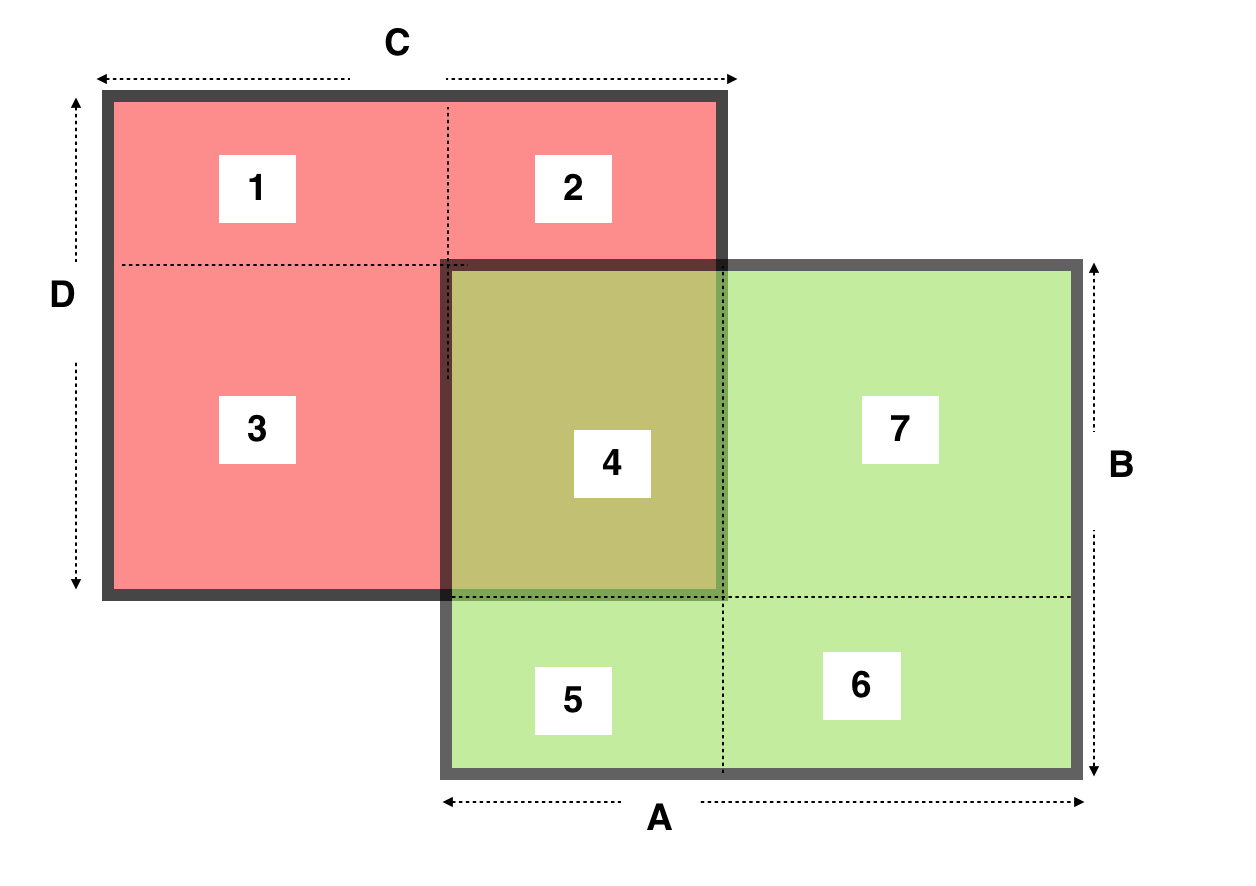
\includegraphics[scale=.45]{oct2pic.png}\\ 
\[
\text{Notice we can write  } (A \times B) \cup (C \times D) \text{ as the union of the disjoint rectangles, labeled 1 to 7 in the figure above.}  
\]
\[
(A \times B) \cup (C \times D) =((A\backslash C) \times (B \backslash D)) \ \cup \ ((A\backslash C^c) \times (B \backslash D)) \ \cup \ ((A\backslash C) \times (B \backslash D^c)) \ \cup \ ((A\backslash C^c) \times (B \backslash D^c)) \ \cup 
\]
\[
((A\backslash C^c) \times (D \backslash B)) \ \cup \ ((C\backslash A) \times (D \backslash B)) \ \cup \ \ ((C\backslash A) \times (B \backslash D^c)) 
\]
From the figure, we can see that all these rectangles are disjoint; thus, $R_i \cup R_j \in \A$.\\ Assume that $\bigcup_{i=1}^{n}R_i \in \A$. Then,  $\bigcup_{i=1}^{n}R_i \cup R_j= \bigcup_{i=1}^n (R_i \cup R_j)$. Our previous conclusion implies that $(R_i \cup R_j) \in \A$. So, since $\bigcup_{i=1}^{n}R_i \in \A$ and $(R_i \cup R_j) \in \A$, $\bigcup_{i=1}^{n+1} (R_i) \in \A$. Thus, $\bigcup_{i=1}^k R_i  \in \A$. \\
Next, to show $R_i^c \in \A$ for any $i$, consider $(A \times B) \cap (C \times D)$ in the figure. Notice $(A \times B) \cap (C \times D)=(A \cap C) \times (B \cap D) \in \A$. Thus, inductively, we can show $\bigcap_{i=1}^n R_i \in \A$. So, by inspection of figure, we can see
\[
R_i^c=\left(\bigcup_{i=1}^n A_i\times B_i \right)^c=\bigcap_{i=1}^n (A_i\times B_i)^c=\bigcap_{i=1}^n\left( (A_i^c\times B_i^c) \cup (A_i\times B_i^c) \cup (A_i^c\times B_i)\right). 
\]
Notice $(A_i^c\times B_i^c), (A_i\times B_i^c), (A_i^c\times B_i)$ are disjoint so $(A_i^c\times B_i^c) \cup (A_i\times B_i^c) \cup (A_i^c\times B_i) \in \A$. Thus, $\bigcap_{i=1}^n\left( (A_i^c\times B_i^c) \cup (A_i\times B_i^c) \cup (A_i^c\times B_i)\right) \in \A$, so $R_i^c \in \A$ for any $i$.\\
Hence, $\A$ is an algebra. 
\end{pf}

\item Prove that if $\mu$ and $\nu$ are $\sigma$-finite then so is $\mu \times \nu$. 
\begin{pf}
	Assume $\mu$ and $\nu$ are $\sigma$-finite. Then, $X=\bigcup_{j=1}^\infty A_j$ with $\mu(A_j)<\infty$ for all $j$ and $Y=\bigcup_{i=1}^\infty B_i$ with $\nu(B_i)< \infty$ for all $i$. Then, $X \times Y=\bigcup_{j=1}^\infty A_j \times \bigcup_{i=1}^\infty B_i=\bigcup_{j=1}^\infty \bigcup_{i=1}^\infty A_j \times B_i$. Since $\mu(A_j)<\infty$ and $\nu(B_i)< \infty$ for all $i, j$, $\mu(A_j)\nu(B_i)<\infty$ for all $i, j$. Therefore, $\mu \times \nu$ is $\sigma$-finte.
\end{pf}
\end{enumerate}

 \section{Section 1.3 (Folland): Complete proof of Theorem 1.9}

 \subsection{October 5 Group Assignment}
Let $(X, \M, \mu)$ be a measure space.

\begin{enumerate}
\item Let $N=\{ S \in M : \mu(S)=0 \}$ and $\overline{M}=\{ E \cup F : E \in M$ and there is $S \in N$ such that $F \subseteq S \}$. Prove that $\overline{M}$ is a $\sa$ that contains $M$.
\begin{pf}
	To show $\overline{M}$ is closed under countable unions, we will start by showing $N$ is closed under countable unions. Consider a disjoint collection of sets, $\{E_i\}_{i=1}^\infty \subset N$. Then, for all $i$, $E_i \in M$ and $\mu(E_i)=0$. Also, because $\mu$ is sub-additive and $E_i\cap E_j = \O$ for all $i\neq j$, $\mu\left(\bigcup_{i=1}^\infty E_i\right)=\sum_{i=1}^\infty\mu(E_i)=\sum_{i=1}^\infty 0=0$. Since $E_i \in M$ for all $i$, $\bigcup_{i=1}^\infty E_i \in M $. Thus, $\bigcup_{i=1}^\infty E_i \in N$ and so $N$ is closed under countable unions.
	Notice $\overline{M}$ is the union of sets from $M$ and $N$. Thus, because $M$ and $N$ are closed under countable unions, $\overline{M}$ is closed under countable unions. \\
	Next, we will show $\overline{M}$ is closed under complements. Consider $E \cup F \in \overline{M}$. Then, $E \in M$ and $F \in N$. Suppose $E \cap N = \O$. 
	\\
	\noindent \textbf{Lemma: $E \cup F=(E\cup N) \cap (N^c \cup F)$}
	\begin{pf}
	First, we will show $E \cup F \subseteq (E\cup N) \cap (N^c \cup F)$. Let $x \in E \cup F$. Then, $x \in E$ or $x \in F$. Suppose $x \in E$. Then, $x \in E \cup N$. Also, since $E \cap N = \O$, $x \in N^c$ so $x \in N^c \cup F$. Thus, $x \in (E\cup N) \cap (N^c \cup F)$. Suppose $x \in F$. Then, $x \in N^c \cup F$. Since $x \in F$ and $E \cup F \in \overline{M}$, $F \in N$ and there exists some $S \in N$ such that $F \subseteq S$. Thus, $x \in N$ and so $x \in E \cup N$. Therefore, $E \cup F \subseteq (E\cup N) \cap (N^c \cup F)$. \\
	Next, we will show $E \cup F \supseteq (E\cup N) \cap (N^c \cup F)$. Let $x \in (E\cup N) \cap (N^c \cup F)$. Then, $x \in E \cup N$ and $x \in N^c \cup F$. If $x \in E$, then $x \in E \cup F$ and we have our desired relation. So, suppose $x \not\in E$. Then, since $x \in E \cup N$, $x \in N$. Since $x \in N$, $x \not\in N^c$. Since $x \in N^c \cup F$, this implies $x \in F$ so that $x \in E \cup F$. Thus, $E \cup F \supseteq (E\cup N) \cap (N^c \cup F)$. 
	\end{pf}

	\noindent By the lemma above, we can write $(E \cup F)^c = ((E\cup N) \cap (N^c \cup F))^c=(E \cup N)^c \cup (N^c \cup F)^c= (E \cup N)^c \cup (N \backslash F) $. $M$ is closed under complements and countable unions, so $E \in M$ and $N \subset M$ implies $E \cup N \in M$ and $(E \cup N)^c \in M$. Also, $N \backslash F \subset N$. Thus, $(E \cup F)^c \in \overline{M}$. 
	\\
	Now, suppose $E \cap N \neq \O$, and consider the following lemma: 
\\	\noindent \textbf{Lemma: If $E \cap N \neq \O$, $E \cup F=(E\cup N\backslash E) \cap ((N \backslash E)^c \cup F \backslash E)$}
	\begin{pf}
	First, we will show $E \cup F\subseteq (E\cup N\backslash E) \cap ((N \backslash E)^c \cup F \backslash E)$. Let $x \in E \cup F$. Then, $x \in E$ or $x \in F$. Suppose $x \in E$. Then, $x \in E\cup N\backslash E$. Since $x \in E$, $x \in (N^c \cup E)=(N \backslash E)^c $. 
	Thus, $x \in (E\cup N\backslash E) \cap ((N \backslash E)^c \cup F \backslash E)$. Suppose $x \in F$, but $x \not\in E$. Then, $x \in F \backslash E$, so $x \in (N \backslash E)^c \cup F \backslash E$. Since $x \in F$ and $E \cup F \in \overline{M}$, there exists some $S \in N$ such that $F \subseteq S$. Thus, $x \in N$. Since $x \not\in E$, $x \in N\backslash E$ so $x \in E \cup N \backslash E$. Therefore, $E \cup F\subseteq (E\cup N\backslash E) \cap ((N \backslash E)^c \cup F \backslash E)$. \\
	Next, we will show $E \cup F \supseteq (E\cup N\backslash E) \cap ((N \backslash E)^c \cup F \backslash E)$. Let $x \in (E\cup N \backslash  E) \cap ((N \backslash E)^c \cup F \backslash E)$.  Then, $x \in (E\cup N\backslash E)$ and $x \in  ((N \backslash E)^c \cup F \backslash E)$. If $x \in E$, then $x \in E \cup F$ and we have our desired relation. So, suppose $x \not\in E$. 
	
	Then, since $x \in E \cup N \backslash E$, $x \in N \backslash E$ and so $x \in N$. Since $x \in N$, $x \not \in N^c$ and so $x \not \in (N\backslash E)^c$. Since $x \in (N\backslash E)^c \cup F \backslash E$,  $x \in F \backslash E$ so that $x \in E$. Thus, $x \in E \cup F$. 
	
	Hence, $E \cup F\supseteq (E\cup N\backslash E) \cap ((N \backslash E)^c \cup F \backslash E)$. 
	\end{pf}
\noindent By the lemma above, we can write $(E \cup F)^c = ((E\cup N\backslash E) \cap ((N \backslash E)^c \cup F \backslash E))^c=(E\cup N\backslash E)^c \cup ((N \backslash E)^c \cup F \backslash E)^c=  (E\cup N\backslash E)^c \cup (N \cap (E \backslash F))$. $M$ is closed under complements and countable unions and intersections, so $E \in M$ and $N\backslash E \subset M$ implies $E \cup N\backslash E \in M$ and $(E\cup N\backslash E)^c \in M$. Also, $N \cap (E \backslash F) \subset N$. Thus, $(E \cup F)^c \in \overline{M}$. 

\end{pf}

\item If $E \cup F \in \overline{M}$ define $\overline{\mu}(E \cup F)= \mu(E)$. Prove that this function is well defined. 
\begin{pf}
Assume $E^{'}\cup F^{'}= E^{''}\cup F^{''}$ with $E^{'}\cup F^{'}$ and $ E^{''}\cup F^{''}$ in $\overline{M}$. Since $E^{'} \subseteq E^{'}\cup F^{'}, \ E^{'} \subseteq E^{''}\cup F^{''}$. Also, since $E^{''}\cup F^{''} \in \overline{M}$, there exists $S^{''} \in N$ such that $F^{''} \subseteq S^{''}$. Thus, $E^{'} \subseteq E^{''}\cup F^{''} \subseteq E^{''}\cup S^{''}$. By monotonicity of $\mu$,  $\mu(E^{'}) \leq \mu(E^{''}\cup F^{''}) \leq \mu(E^{''}\cup S^{''})$. Also, by subadditivity of $\mu$, $\mu(E^{''}\cup S^{''})\leq \mu(E^{''}) + \mu(S^{''})$. Since $S^{''} \in N$, $\mu(S^{''})=0$. Thus, $\mu(E^{'}) \leq \mu(E^{''})$. \\
Similarly, $E^{''} \subseteq E^{''}\cup F^{''}, so \ E^{''} \subseteq E^{'}\cup F^{'}$. Also, since $E^{'}\cup F^{'} \in \overline{M}$, there exists $S^{'} \in N$ such that $F^{'} \subseteq S^{'}$. Thus, $E^{''} \subseteq E^{'}\cup F^{'} \subseteq E^{'}\cup S^{'}$. By monotonicity of $\mu$,  $\mu(E^{''}) \leq \mu(E^{'}\cup F^{'}) \leq \mu(E^{'}\cup S^{'})$. Also, by subadditivity of $\mu$, $\mu(E^{'}\cup S^{'})\leq \mu(E^{'}) + \mu(S^{'})$. Since $S^{'} \in N$, $\mu(S^{'})=0$. Thus, $\mu(E^{''}) \leq \mu(E^{'})$.\\
Hence $\mu(E^{'})=\mu(E^{''})$ and by definition of $\overline{\mu}$, $\mu(E^{'})=\overline{\mu}(E^{'}\cup F^{'})$ and $\mu(E^{''})=\overline{\mu}(E^{''}\cup F^{''})$ which implies $\overline{\mu}(E^{'}\cup F^{'})=\overline{\mu}(E^{''}\cup F^{''})$. Thus, $\overline{\mu}$ is well defined. 
\end{pf}
\item Prove that $\overline{\mu}$ is a measure on $\overline{M}$ and that the measure is complete.
\begin{pf}
We will prove $\overline{\mu}$ is a measure on $\overline{M}$. Note $\O \in M$ and since $\mu(\O) = 0$ $\O \in N$. Thus, $\overline{\mu}(\O \cup \O)= \mu(\O)=0$. Now, we will show $\overline{\mu}$ is countably additive. Consider a disjoint collection of sets in $\overline{M}$, $\{ A_i \}_{i=1}^\infty$. Then, for all $i$, $A_i = E_i \cup F_i$ for some $E_i \in M$ and where $F_i \subseteq S_i$ for some $S_i \in N$. Then, 
\[
\overline{\mu}\left(\bigcup_{i=1}^\infty A_i\right) = \overline{\mu}\left(\bigcup_{i=1}^\infty E_i \cup F_i \right) = \overline{\mu}\left(\bigcup_{i=1}^\infty E_i \cup \bigcup_{i=1}^\infty F_i \right)
\]
$M$ and $N$ are closed under countable unions, so $\bigcup_{i=1}^\infty E_i \in M$ and $ \bigcup_{i=1}^\infty F_i \subseteq \bigcup_{i=1}^\infty S_i \in N$. By definition of $\overline{\mu}$, because $E_i's $ are disjoint and because $\mu$ is countably additive we can write 
\[
\overline{\mu}\left(\bigcup_{i=1}^\infty E_i \cup \bigcup_{i=1}^\infty F_i \right) = {\mu}\left(\bigcup_{i=1}^\infty E_i \right) = \sum_{i=1}^\infty\mu(E_i)= \sum_{i=1}^\infty\overline{\mu}(E_i \cup F_i) =\sum_{i=1}^\infty\overline{\mu}(A_i).\]
Thus, $\overline{\mu}$ is countably sub-additive. 
\end{pf}
\begin{pf}
Next, we will prove $\overline{\mu}$ is a complete measure on $\overline{M}$. To prove this we must show that the domain of $\overline{\mu}$ contains all subsets of null sets. Suppose $E \cup F$ is a $\overline{\mu}$-null set.  Since $E \cup F$ is a $\overline{\mu}$-null set, $\overline{\mu}(E \cup F) = 0 = \mu(E)$. Thus, $E$ is a $\mu$-null set. Also, if $E \cup F \in \overline{M}$, then $F \subseteq S \in N$, so $0 \leq \mu(E \cup S) \leq \mu(E) + \mu(S) = 0$. Thus, $\mu(E \cup S) = 0$ so $E \cup S$ is a $\mu$-null set. Consider any $A \subseteq E \cup F$. The subset relation is transitive, so $A \subseteq E \cup S$. Thus, $A$ is a subset of some element in $N$, so since $\O \in M$, $\O \cup A \in N$, so we can write $\overline{\mu}(A)=\overline{\mu}(\O \cup A)= \mu(\O)=0$. Thus, $A \in \overline{M}$. \\
\noindent **Sources used: \url{http://www.math.ubc.ca/~marcus/Math507420/Math507420_HW2_solns_2013.pdf} and \url{https://proofwiki.org/wiki/Completion_Theorem_(Measure_Spaces)}
\end{pf}


\item Prove that if $\sigma$ is a complete measure on $\overline{M}$ such that $\sigma |_M=\mu$, then $\sigma = \overline{\mu}$. 
\begin{pf}
Let $\sigma$ be a complete measure on $\overline{M}$ such that $\sigma |_M=\mu$. Consider any $E \cup F \in \overline{M}$. Then, $E \subset E \cup F \subset E \cup S$ for some $S \in N$. Thus, by monotonicity of $\sigma$, 
$\sigma(E) \leq \sigma(E \cup F) \leq \sigma(E \cup S)$. Since $E \in M$ and $S \in M$, $E \cup S \in M$ and we can write $\sigma(E \cup S)= \mu(E \cup S)$ and by subadditivity of $\mu$, $\mu(E \cup S)\leq \mu(E) + \mu(S)$. $S \in N$, so $\mu(S)=0$. Thus, $\sigma(E) \leq \sigma(E \cup F) \leq \sigma(E \cup S) = \mu(E \cup S) \leq \mu(E)=\sigma(E)$ since $E \in M$. Thus, $\sigma(E) \leq \sigma(E \cup F) \leq \sigma(E)$ so $\sigma(E \cup F)= \mu(E)=\overline{\mu}(E \cup F)$. Thus, $\sigma = \overline{\mu}$.\\
**Source used: \url{ http://faculties.sbu.ac.ir/~shahrokhi/M-P.pdf }
\end{pf}
\end{enumerate}

 \section{Section 1.5 (Folland): Borel Measures on the Real Line}
 \subsection{Section 1.5 Definitions and Theorems}
 \begin{dfn}A Borel measure is any measure $\mu$ defined on the $\sa$ of Borel sets. 
\end{dfn}

\begin{thm} If $F: \R \rightarrow \R$ is any increasing, right continuous function, there is a unique Borel measure $\mu_F$ on $\R$ such that $\mu_F((a,b])=F(b)-F(a)$ for all $a,b$. \\
If $G$ is another such function, we have $\mu_F= \mu_G$ iff $F-G$ is constant.\\
Conversely, if $\mu$ is a Borel measure on $\R$ that is finite on all bounded Borel sets and we define
\[ F(x) = \left\{
\begin{array}{ll}
	\mu((0, x]) & \text{ if } x>0\\
	0 & \text{ if } x=0\\
	-\mu((x, 0]) & \text{ if } x<0
\end{array} \right. 
\]	
then $F$ is increasing and right continuous and $\mu=\mu_F$.
\end{thm}

\begin{dfn}[$\B_\R$]
	Borel $\sa$: generated by family of open sets in $\R$ (or closed, half-open, open rays, closed rays
\end{dfn}

\begin{dfn}[Lebesgue-Stieltjes measure]
	For any $E \in \M_\mu$, \[
	\mu(E) = \inf \left\{ \sum_1^\infty \mu((a_j, b_j)): E \subset  \bigcup_1^\infty (a_j, b_j)  \right\}.
	\]
\end{dfn}

\begin{thm}
If $E \in \M_\mu$, then \[
\mu(E) = \inf \{ \mu(U): U \supset E, \ U \text{ open} \} = \sup \{ \mu(K) : K \subset E, \ K \text{ compact} \}
\]
\end{thm}

\begin{thm}
\[
E \subset \R. \quad E \in \M_\mu \iff E = V \slash N_1, \ V \text{ is }  G_\delta, \mu(N_1)= 0 \iff E = H \cup N_2, \ H \text{ is }  F_\sigma, \ \mu(N_2)=0.
\]	
\end{thm}

\begin{dfn}[Lebesgue measure]
	Complete measure $\mu_F$ associated to the function $F(x) = x$ for which the measure of an interval is simply its length. Denoted $m$.
\end{dfn}
\begin{rmk}
$m$ is invariant under translations, simple behavior under dilations: $m(E + s) = m(E)$ and $m(rE) = |r|m(E)$	
\end{rmk}

\begin{rmk}
Every singleton set in $\R $ has Lebesgue measure zero.	Every countable set has Lebesgue measure zero. 
\end{rmk}





 
 
 \subsection{October 9 Group Assignment}
\begin{enumerate}
\item Let $\delta_i$ denote the Dirac measure concentrated on $i$, in other words: \\
\[
\delta_i(E)= \left\{
\begin{array}{ll} 
      1 & i \in E \\
      0 & i \not\in E 
\end{array} 
 \right. 
\]
Find the distribution function for the measure $\sum_{i=1}^{10} i^2 \delta_i$.\\
First notice that 
\[
\begin{array}{c}
1^2 \delta_1(\{1\})=1 \\
2^2 \delta_2(\{2\})=4 \\
3^2 \delta_3(\{3\})=9 \\
\vdots \\
10^2 \delta_{10}(\{ 10 \}) = 100 \\
\end{array}
\]
Also, 
\begin{eqnarray*}
F(1)&=&\sum_{i=1}^{10} i^2 \delta_i((0,1])=1 \\
F(2)&=&\sum_{i=1}^{10} i^2 \delta_i((0,2])=1+4 =5 \\
F(3)&=&\sum_{i=1}^{10} i^2 \delta_i((0,3])=1+4+9=14  \\
 & & \vdots \\
F(10)&=&\sum_{i=1}^{10} i^2 \delta_i((0,10]) = 1+4+9 + \cdots + 100
\end{eqnarray*}
Thus, 
\[
F(E)= \left\{
\begin{multlined} 
     \sum_{i=1}^{\lfloor x \rfloor}i^2 \qquad x <10 \\
      \vspace{.005cm}\\
 \sum_{i=1}^{10}i^2 \qquad x \geq 10
\end{multlined} \right.
\]
\item Let $F$ be increasing and right continuous; let $\mu_F$ denote the associated measure. 
\\
\begin{center}\fbox{ Prove $\mu_F(\{a\})=F(a)-F(a-)$ }\end{center}
\[
\text{First, notice } \{a\} = \bigcap_{n=1}^\infty \left(a - \frac{1}{n}, a\right]. \  \text{So, } \mu_F (\{a\}) = \mu_F \left( \bigcap_{n=1}^\infty \left(a - \frac{1}{n}, a\right] \right).
\]


 \[
\text{Measures are continuous from above so, } \mu_F (\{a\}) = \mu_F \left( \bigcap_{n=1}^\infty \left(a - \frac{1}{n}, a\right] \right) = \lim_{n \rightarrow \infty}\mu_F \left( \left(a - \frac{1}{n}, a\right] \right)
\]
\[
= \lim_{n \rightarrow \infty} F(a) - F\left(a - \frac{1}{n}\right) = F(a) - \lim_{n \rightarrow \infty} F\left(a - \frac{1}{n} \right)= F(a)-F(a-) .\vspace{.75cm}
\]
\begin{center}\fbox{Prove $ \ \mu_F((a,b))=F(b-)-F(a)$} \end{center}
\[
\text{First, notice } (a,b) = \bigcup_{n=1}^\infty \left(a, b- \frac{1}{n}\right]. \  \text{ So, } \mu_F ((a,b)) = \mu_F \left( \bigcup_{n=1}^\infty \left(a, b- \frac{1}{n}\right] \right). \text{ Measures are continuous}
\]


 \[
 \text{  from below so,  } \mu_F ((a,b)) = \mu_F \left( \bigcup_{n=1}^\infty \left(a, b- \frac{1}{n}\right] \right)=\lim_{n \rightarrow \infty} \mu_F \left(\left(a, b- \frac{1}{n}\right] \right)
\]
\[
= \lim_{n \rightarrow \infty} \left( F\left(b - \frac{1}{n}\right) - F\left(a\right) \right) = \lim_{n \rightarrow \infty} \left( F\left(b - \frac{1}{n}\right) \right) - F\left(a\right) =F(b-)-F(a) .
\]
%%%%%%%%%%%%%%%%%%%
\begin{center}\fbox{ Prove $  \ \mu_F([a,b))=F(b-)-F(a-)$}\end{center}
\[
\text{First, notice } [a,b) = \{a\} \cup (a,b)  \text{ and } \{a\} \cap (a,b)= \O . \ \mu_F \text{ is a pre-measure, so  } \mu_F ([a,b)) = \mu_F(\{a\} \cup (a,b))
\]
 \[
 = \mu_F(\{ a \}) + \mu_F((a,b)). \text{ From the two previous conclusions, we have }
\]
\[ \mu_F(\{ a \}) + \mu_F((a,b)) =F(a)-F(a-)+F(b-)-F(a)=F(b-)-F(a-).
\]
\begin{center}\fbox{Prove $ \ \mu_F([a,b])=F(b)-F(a-)$}\end{center}
\[
\text{First, notice } [a,b] = \{b\} \cup [a,b)  \text{ and } \{b\} \cap [a,b)= \O . \ \mu_F \text{ is a pre-measure, so  } \mu_F ([a,b]) = \mu_F(\{b\} \cup [a,b))
\]
 \[
 = \mu_F(\{ b \}) + \mu_F([a,b)). \text{ From part 1 and 3 of this exercise, we have }
\]
\[ \mu_F(\{ b \}) + \mu_F([a,b)) =F(b)-F(b-)+F(b-)-F(a-)=F(b)-F(a-).
\]


\item Use the previous exercise to describe a Borel measure so that the four quantities given are different where $a = 0$ and $b = 1$. \\
 Consider the function
 \[
 F(x)= \left\{
 \begin{array}{ll}
 	1 & -\infty \leq x < 0\\
 	3 & 0 \leq x < \frac{1}{2}\\
 	9 & \frac{1}{2} \leq x < 1\\
 	27 & 1 \leq x < \infty
 \end{array}
 \right.
 \]
 If $F$ is as defined above with $a=0$, $b = 1$, then, 
 \[
  \begin{array}{lll}
 	F(a)-F(a-)=F(0) -F(0-)& = 3-1&=2\\
 	F(b-)-F(a) =F(1-) -F(0)& = 9-3&=6\\
 	F(b-)-F(a-) =F(1-) -F(0-)& = 9-1&=8\\
 	F(b)-F(a-) =F(1) -F(0-)& = 27-1&=26
 \end{array}.
 \]
 
\end{enumerate}


\subsection{October 12 Group Assignment}
Exercise 32 from $\S 1.5$. 
\begin{enumerate}
\item 	Prove that 
\[ \prod_{j=1}^\infty(1 - a_j)> 0 \text{ if and only if } \sum_{j=1}^\infty a_j < \infty 
\]
\begin{pf}
	To prove the desired statement, we will use the limit comparison test to  show that $\sum_{j=1}^\infty a_j$ converges if and only if $\sum_{j=1}^\infty \log(1-a_j)$ converges. \\
	$(\Leftarrow)$ Suppose $\sum a_j$ converges. If we assume $a_j\rightarrow 0$, 
	\[
	\lim_{j\rightarrow \infty}\frac{a_j}{\log(1-a_j)}= \lim_{x \rightarrow 0}\frac{x}{\log(1-x)}. 
	\]
	 \[
\text{Applying L’Hospital’s Rule, } \lim_{x \rightarrow 0}\frac{x}{\log(1-x)}=\lim_{x \rightarrow 0}\frac{1}{\frac{-1}{1-x}}=-1.
	\]
	Thus, if $a_j\rightarrow 0$, $\lim_{j\rightarrow \infty}\frac{a_j}{\log(1-a_j)}=-1$. By the limit comparison test, 
	\[
	\lim_{n\rightarrow \infty}\sum_{j=1}^n a_j \text{ converges if and only if } \lim_{n\rightarrow \infty}\sum_{j=1}^n \log(1-a_j) \text{ converges. Thus, }
	\]
	\[ \text{ since } \log(1-a_j)<0 \text{ for all } j. \  \sum_{j=1}^\infty \log(1-a_j)> -\infty \text{ if and only if } \sum_{j=1}^\infty a_j < \infty 
\]
Since $\sum_{j=1}^\infty \log(1-a_j)> -\infty $, let $\sum_{j=1}^\infty \log(1-a_j)=k$ for $-\infty < k < 0$. Equivalently, 
\[
10^{\sum_{j=1}^\infty \log(1-a_j)}=10^k \text{ implies }  \prod_{j=1}^\infty(1 - a_j)=10^k>0.
\]
($\Rightarrow$) Assume $\prod_{j=1}^\infty(1 - a_j)> 0 $. Then, let $\prod_{j=1}^\infty(1 - a_j)=k$ for $k>0$. Then,
\[
\log\left(\prod_{j=1}^\infty(1 - a_j)\right)=\sum_{j=1}^\infty \log(1-a_j)=\log(k)>-\infty \text{ implies } \lim_{n\rightarrow \infty}\sum_{j=1}^n \log(1-a_j) \text{ converges. }
\]
Suppose $ \lim_{j\rightarrow \infty} \log(1-a_j) =0$. Since $\log$ is a continuous function, we can write $ \log(1-\lim_{j\rightarrow \infty} a_j)=0$ which implies $\lim_{j\rightarrow \infty} a_j=0$ Then, as shown above, the limit comparison test implies $\lim_{n\rightarrow \infty}\sum_{j=1}^n a_j$ converges so $\sum_{j=1}^\infty a_j< \infty$.
\end{pf}

\item Given $\beta \in (0,1)$, exhibit a sequence $\{a_j\}$ such that $\prod(1-a_j)=\beta$.  \\
If $\prod(1-a_j)=\beta$, then $\ln\left(\prod(1-a_j)\right)=\ln\beta$ and $\sum\ln(1-a_j)=\ln\beta$. From part (1), we know that $\sum\ln(1-a_j)$ converges implies $\sum a_j$ converges. Also, $\ln\beta= \sum \frac{\ln \beta}{2^j}$ so $\sum\ln(1-a_j)=\sum \frac{\ln \beta}{2^j}$ implies
\[
e^{\ln(1-a_j)}=e^{\frac{\ln \beta}{2^j}}. \text{ Equivalently, } 1-a_j=e^{\ln \beta^{-2^j}}=\beta^{-2^j}.
\] 
Thus, the sequence $a_j=1-\beta^{-2^j}$ satisfies $\prod(1-a_j)=\beta$.
\end{enumerate}

\section{Section 2.1 (Folland): Measurable Functions}
\subsection{Section 2.1 Definitions and Theorems}
 \begin{rmk}
Any mapping $f: X \rightarrow Y$ between two sets induces a mapping $f^{-1}: \sP (Y) \rightarrow \sP(X)$ defined by $f^{-1}(E)= \{ x \in X : f(x) \in E \}$ which preserves unions, intersections, and complements. Thus, if $\sN$ is a $\sa$ on $Y$, then $\{ f^{-1}(E) : E \in \sN \}$ is a $\sa$ on $X$
\end{rmk}

\begin{dfn}[measurable functions]
	If $(X, \M)$ and $(Y, \sN)$ are measurable spaces, a mapping $f: X \rightarrow Y$ is called $(\M, \sN)$-measurable if $f^{-1}(E) \in \M$ for all $E \in \sN$.
\end{dfn}
\begin{prop}
If $\sN$ is generated by $\E$, then $f$ is $(\M, \sN)$-measurable iff $f^{-1}(E) \in \M$ for all $E \in \E$	
\end{prop}

\begin{cor}
$X, Y$ are topological spaces, every continuous $f: X \rightarrow Y$ is $(\B_x, \B_y) $-measurable. 	
\end{cor}

\begin{prop} $(X, \M)$ is a measure space and $f: X \rightarrow \R$, then \[
f \text{ is } \M-\text{ measurable } \iff f^{-1}((a, \infty )) \in \M \text{ for for all } a \in \R \iff f^{-1}([a, \infty )) \in \M \text{ for for all } a \in \R 
\]
\[
\iff  f^{-1}((- \infty, a )) \in \M \text{ for for all } a \in \R \iff f^{-1}((- \infty , a]) \in \M \text{ for for all } a \in \R 
\]
	
\end{prop}

\begin{dfn}[simple functions]
A finite linear combination with complex coefficients of characteristic functions of sets in $\M$.	
\end{dfn}

\begin{dfn}[standard representation of $f$]
\[
f = \sum_1^n z_j \chi_{E_j}, \text{ where } E_j = f^{-1}(\{ z_j \}) \text{ and range}(f)= \{ z_1, \dots, z_n \}.
\]	
\end{dfn}



 
 
\subsection{October 14 Group Assignment}
\begin{enumerate}
\item (exercise 8, $\S 2.1$): Prove that if $f : \R \rightarrow \R$ is monotone then it is measurable.
\begin{pf}
	Let $f: \R \rightarrow \R$ be monotone.  By Proposition
2.3 in Page 44, it suffices to show that for any $a \in \R$, we have $f^{−1}((a, \infty))$ is Borel measurable. WLOG, assume $f$ is increasing. Let $x^{'}=\inf \{x : f(x) >a  \}$\\
	\textbf{Case 1:	Suppose $f(x^{'}) \leq a$.}
 We will show $f^{-1}((a, \infty))=(x^{'}, \infty)$. First, show $f^{-1}((a, \infty))\subseteq (x^{'}, \infty)$. Let $x \in f^{-1}((a, \infty))$. Then, $f(x)>a$. Since $x^{'}=\inf \{x : f(x) >a  \}$, $x^{'}<x$. Thus, $x \in (x^{'}, \infty)$. \\
	Next, show $f^{-1}((a, \infty))\supseteq (x^{'}, \infty)$. Let $x \in (x^{'}, \infty)$. Then, $x>x^{'}$.  Since $x^{'}=\inf \{x : f(x) >a  \}$ and $x>x^{'}$, there exists some $x_0 \in \R$ such that $x>x_0>x^{'}$ and $f(x_0)>a$. $f$ is monotone, so $f(x)>f(x_0)$. Thus, $f(x)>a$ which implies $x \in f^{-1}((a, \infty))$.  \\
\textbf{Case 2: Suppose $f(x^{'}) > a$}. We will show $f^{-1}((a, \infty))=(x^{'}, \infty)$. First, show $f^{-1}((a, \infty))\subseteq (x^{'}, \infty)$. Let $x \in f^{-1}((a, \infty))$. Then, $f(x)>a$. Since $x^{'}=\inf \{x : f(x) >a  \}$, $x^{'}<x$. Thus, $x \in (x^{'}, \infty)$. \\
	Next, show $f^{-1}((a, \infty))\supseteq (x^{'}, \infty)$. Let $x \in (x^{'}, \infty)$. Then, $x>x^{'}$.  Since $f$ is monotone, so $f(x)>f(x^{'})> a$. Thus, $f(x)>a$ which implies $x \in f^{-1}((a, \infty))$.  \\
	\textbf{Case 3: Suppose $f(x^{'}) =\infty$}. We will show $f^{-1}((a, \infty))=\O$. If $f(x^{'}) =\infty$, $f(\inf\{x : f(x)>a\}) =\infty$ which implies $\inf\{x : f(x)>a\} =\infty$ so $\{x : f(x)>a\}=\O$. Thus, $f^{-1}((a, \infty))=\O$.\\
	\textbf{Case 4: Suppose $f(x^{'})=-\infty$}. We will show $f^{-1}((a, \infty))=\R$. If $f(x^{'}) =-\infty$, $f(\inf\{x : f(x)>a\}) =-\infty$ which implies $\inf\{x : f(x)>a\} =-\infty$ so $\{x : f(x)>a\}=\R$. Thus, $f^{-1}((a, \infty))=\R$.\\
	Hence, for any $a \in \R$, we have $f^{−1}((a, \infty))$ is Borel measurable, so $f$ is measurable. 
\end{pf}
\item (exercise 5, $\S 2.1$):	If $X=A \cup B$ with $A, B \in \M$, then a function $f$ on $X$ is measurable if and only if $f$ is measurable on $A$ and $B$. 
\begin{pf}
Let $f: (X, \M) \rightarrow (Y, \sN)$.
	First, assume $f$ is measurable on $X=A \cup B\in \M$. Then, for all $N \in \sN$, $f^{-1}(N) \in \M$. Since $A, B \in \M$, $f^{-1}(N) \cap A \in \M$ and $f^{-1}(N) \cap B \in \M$ for all $N \in \sN$. Thus, $f$ is measurable on $A$ and $f$ is measurable on $B$.\\
	Next, assume $f$ is measurable on $A$ and $f$ is measurable on $B$. Then, for all $N \in \sN$, $f^{-1}(N)\cap A \in \M$ and  $f^{-1}(N)\cap B \in \M$. This implies $(f^{-1}(N)\cap A) \cup (f^{-1}(N)\cap B) \in \M$. Since $(f^{-1}(N)\cap A) \cup (f^{-1}(N)\cap B)=f^{-1}(N) \cap (A \cup B)$, $f$ is measurable on $A \cup B$. 

\end{pf}
\url{http://www.math.brown.edu/~rkenyon/teaching/2009/2210/Set3.pdf} 


\end{enumerate}

\subsection{October 16 Group Assignment}
\begin{enumerate}
\item (exercise 3, $\S 2.1$): If $\{f_n\}$ is a sequence of measurable functions then the set $\{x : \lim_{n \rightarrow \infty} f_n(x) $ exists$\}$ is measurable.
 \begin{pf}
Assume $\{f_n\}$ is a sequence of measurable functions. Consider $\{x : \lim_{n \rightarrow \infty} f_n(x) $ exists$\}$. If $\lim_{n \rightarrow \infty} f_n(x) $ exists, $\limsup f_n(x)=\lim f_n(x)$. Thus, \[
\{x : \lim_{n \rightarrow \infty} f_n(x) \text{ exists}\}= \{x : \limsup f_n(x)=\lim f_n(x)\}.
\]
By, proposition 2.7, $g_3(x)=\limsup f_n(x)$ and $g_4(x)=\lim f_n(x)$ are measurable functions. Define $g= g_3 - g_4$. Then, $g$ is a measurable function. If $g(x)=0$, then $x \in \{x : \lim_{n \rightarrow \infty} f_n(x) $ exists$\}$. Since $g$ is measurable, $g^{-1}(\{0\})=\{x : \lim_{n \rightarrow \infty} f_n(x) $ exists$\}$ is measurable. 
 \end{pf}
\item (exercise 6, $\S 2.1$): Show by example that there is an uncountable set $A$ and for each $a \in A$ a measurable function $f_a$, but $\sup \{f_\alpha : \alpha \in A\}$ is not measurable.  \\	
Consider the set $N_r$ constructed in section 1.1.  Then $N_r$ is an uncountable set and therefore not measurable. However, for every $r \in \Q\cap[0,1)$ and $x \in N$ (where $N$ was defined as the subset of $[0,1)$ containing exactly one member of the equivalence classes defined by $x \sim y$ iff $x-y \in \Q$. Singletons are measurable, so, from page 46 of Folland, the indicator functions $\chi_{\{x+r\}}$ and $\chi_{\{x_r-1\}}$ are measurable for all $r \in \Q\cap [0,1)$ and $x \in N\cap [0,1-r)$ or $x \in N\cap [1-r,1)$. Notice $\sup\{ \chi_{\{x+r\}}, \chi_{\{x+r-1\}}: r \in \Q\cap [0,1)$ and $x \in N\cap [0,1-r)$ or $x \in N\cap [1-r,1) \}=\chi_{N_r}$ But, $ \chi_{N_r}$ is not measurable because $N_r$ is not measurable. 
\end{enumerate}

\section{Section 2.2 (Folland): Integration of Non-Negative Functions}
\subsection{Section 2.2 Definitions and Theorems}
 Fix a measure space $(X, \M, \mu)$.
\begin{dfn}[$L^+$]
The space of all measurable functions from $X$ to $[0, \infty]$.
\end{dfn}

\begin{dfn} If $\phi$ is a simple function in $L^+$ with standard representation
 \[ \phi = \sum_1^n a_j \chi_{E_j}, \text{  then,  }  
\int \phi \ d \mu = \sum_1^n a_j \mu(E_j).
\]	
\end{dfn}

\begin{rmk}
\[
\int_A \phi d \mu = \int_A \phi = \int_A \phi(x) d \mu(x) = \int \phi \ \chi_A \ d \mu
\]	
\end{rmk}

\begin{prop}
Let $\phi$ be simple functions in $L^+$, then $A \rightarrow \int_A \phi d \mu$ is a measure on $\M$.	
\end{prop}

\begin{thm}[monotone convergence theorem]
If $\{ f_n \}$ is a sequence in $L^+ $ such that $f_j \leq f_{j+1}$ for all $j$, and $f = \lim_{n \rightarrow \infty} f_n $, then $\int f = \lim_{n \rightarrow \infty} \int f_n$	
\end{thm}

\begin{thm}[Fatou's Lemma]
	If $\{f_n\}$ is any sequence in $L^+$, then 
	\[
	\int(\liminf f_n) \leq \liminf \int f_n.
	\]
\end{thm}

\begin{cor}
If $\{ f_n \} \subset L^+$, $f \in L^+$, and $f_n \rightarrow f$ a.e., then $\int f \leq \liminf \int f_n$.	
\end{cor}

\begin{prop}
If $f \in L^+$ and $\int f < \infty$, then $\{ x : f(x) = \infty \}$ is a null set and $\{ x: f(x)>0  \}$ is $\sigma$-finte.	
\end{prop}







  
\subsection{October 19 Group Assignment}

\begin{enumerate}
\item Prove if $\varphi$ and $\psi$ are simple functions, then $\varphi + \psi$ and $\varphi \cdot \psi$ are simple functions.	
\begin{pf}
Assume 	$\varphi$ and $\psi$ are simple functions. Then, $\varphi=\sum_{j=1}^{n}z_j\chi_{E_j}$ and $\psi=\sum_{i=1}^{m}\alpha_i\chi_{A_i}$. Then, $\varphi$ and $\psi$ are measurable. The sum of measurable functions is a measurable function, so $\varphi + \psi$ is measurable. Since $\varphi$ and $\psi$ are simple, their range is finite. Let ran$\psi=\{a_i\}_{i=1}^n$ and ran$\varphi=\{ b_j \}_{j=1}^m$ The range of $\varphi + \psi \subseteq \bigcup_{j=1}^m (\{a_i\}_{i=1}^n+b_j)$. Thus, $\psi + \varphi$ is simple. \\
Similarly, if $\varphi$, $\psi$ are measurable, then $\varphi \cdot \psi$ is measurable. Also, the range of $\varphi \cdot \psi \subseteq \bigcup_{j=1}^m (\{a_i\}_{i=1}^n\cdot b_j)$ which is finite. Thus, $\varphi \cdot \psi$ is simple. 
\end{pf}

 \url{http://math.sfsu.edu/schuster/Assignment_08_03.pdf} 
\item Assume that $(X, \M, \mu)$ is complete.
(a) If $f$ is $\M$-measurable functions and $f=g \ \mu$ almost everywhere, then $g$ is $\M$-measurable.
\begin{pf}
	Assume $f$ is a $\M$-measurable function and $f=g \ \mu$ almost everywhere. Define $A=\{ x: f(x)=g(x)\}$ and $B=\{x : f(x) \neq g(x)\}$. Because $f$ is measurable $f^{-1}((a,\infty)) \cap A \in \M$. Also, $f(x)=g(x)$ for all $x \in A$ so $f^{-1}((a,\infty)) \cap A =g^{-1}((a, \infty)) \cap A\in \M$.  Since $g=f \ \mu$ almost everywhere, $\mu(B)=0$. Additionally, $\mu$ is complete, so $\mu(g^{-1}((a,\infty))\cap B)\leq \mu(B)=0$. Thus, $\mu(g^{-1}((a,\infty))\cap B)=0$ implies $g^{-1}((a,\infty))\cap B \in \M$. Notice $X = A \cup B$, so by exercise 5 in $\S 2.1$, $g$ is measurable.  \end{pf}

(b) If $f_n$ is a sequence of $\M$-measurable functions such that $f_n \rightarrow f \ \mu$-almost everywhere, then $f$ is $\M$-measurable. 
 \begin{pf}
 Assume $f_n$ is a sequence of $\M$-measurable functions such that $f_n \rightarrow f \ \mu$ almost everywhere. Define $A=\{ x: f_n(x) \rightarrow f(x) \}$ and $B=\{x : f_n(x) \not\rightarrow f(x)\}$. Because $f_n$ are measurable $f_n^{-1}(N) \cap A \in \M$ for all $N \in \B_\R$. Also, $f_n(x) \rightarrow f(x)$ for all $x \in A$ so $\lim_{n\rightarrow \infty}f_n^{-1}(N) \cap A =f^{-1}(N) \cap A\in \M$.  Since $f_n(x) \rightarrow f(x) \ \mu$ almost everywhere, $\mu(B)=0$. Additionally, $\mu$ is complete, so $\mu(f^{-1}(N)\cap B)\leq \mu(B)=0$. Thus, $\mu(f^{-1}(N)\cap B)=0$ implies $f^{-1}(N)\cap B \in \M$. Notice $X = A \cup B$, so by exercise 5 in $\S 2.1$, $f$ is measurable.	
 \end{pf}
\end{enumerate}



\subsection{October 21 Group Assignment}
\begin{enumerate}
	\item If $f \in L^+$, let $\lambda(E)=\int_E f d\mu$ for $E \in \M$. Then, $\lambda$ is a measure on $\M$, and for any $g \in L^+$, $\int g \ d\lambda=\int fg\  d \mu$.
\begin{pf}
	First, we will show that $\lambda$ is a measure. Notice 
	\[
	\lambda(\O) = \mathop{\mathlarger{\int}_{\O}}f \ d\mu = \mathop{\mathlarger{\int}}f \chi_{\O} \ d\mu =\mathlarger{\int}f\cdot0 \ d\mu=0\text{. Thus, }\lambda(\O)=0.
	\] Next consider a disjoint collection of sets $\{E_j\}_{i=1}^\infty \subset \M$. Then, 
	\[
	\lambda\left( \bigcup_{j=1}^\infty E_i \right)=\mathop{\mathlarger{\int}_{\bigcup_{j=1}^\infty E_i}}f \ d\mu=\mathop{\mathlarger{\int}}f \mathlarger{\chi}_{\ _{\{\bigcup_{j=1}^\infty E_i\}}} \ d\mu= \mathop{\mathlarger{\int}}f \sum_{i=1}^\infty \mathlarger{\chi}_{\ _{E_i}} \ d\mu
	\]
	\[
	= \sum_{i=1}^\infty\mathop{\mathlarger{\int}}f\mathlarger{\chi}_{\ _{E_i}} d\mu=\sum_{i=1}^\infty\mathop{\mathlarger{\int}_{E_i}}f d\mu=\sum_{i=1}^\infty\lambda(E_i).
	\]
	Therefore $\lambda$ is countably sub-additive over disjoint unions; $\lambda$ is a measure.\\
	Next, by Theorem 2.10, $g \in L^+$ implies there is a sequence $\{g_j\}$ of simple functions such that $0 \leq g_1 \leq g_2 \leq \cdots \leq g$ such that $g_j \rightarrow g$ pointwise. Since $g_j$ are simple functions, for all $j$ we can write $g_j=\sum_{i=1}^nz_i \chi_{E_i}$ for $E_i=g_j^{-1}(\{z_i\})$ where range$(g_j)=\{z_1, z_2, \cdots, z_n\}$. Then, for all $g_j$ we have 
	\[
	\begin{array}{lll}
		\vspace{5mm}
	\mathlarger{\int}g_j \ d\lambda & = \sum\limits_{i=1}^n z_i \lambda(E_i) & \text{ definition of integral of simple functions on p. 49}\\
	\vspace{5mm}
	 &= \sum\limits_{i=1}^n z_i \mathop{\mathlarger{\int}_{E_i}}f d\mu &\text{ definition of } \lambda \\
	 \vspace{5mm}
	 &= \mathop{\mathlarger{\int}_{E_i}}\sum\limits_{i=1}^n z_i f d\mu & \\
	 	\vspace{5mm}
	 	 &= \mathop{\mathlarger{\int}}\sum\limits_{i=1}^n z_i \mathlarger{\chi}_{\ _{E_i}} f d\mu & \\
	 	\vspace{5mm}
	 	 &= \mathop{\mathlarger{\int}}g_j f d\mu & \\
	\end{array}
	\]
	Then, by the Monotone Convergence Theorem, since $g_j \rightarrow g$, 
	\[
\mathlarger{\int}g\ d\lambda =	\lim_{j\rightarrow \infty}\mathlarger{\int}g_j \ d\lambda =	\lim_{j\rightarrow \infty}\mathlarger{\int}g_j f d\mu =	\mathlarger{\int}\lim_{j\rightarrow \infty} g_j f d\mu=\mathlarger{\int} g f d\mu
	\]
\end{pf}
	\item If $f \in L^+$ and $\mathlarger{\int} f < \infty$ for every $\epsilon>0$ there exists $E \in \M$ such that $\mu(E)< \infty$ and $\mathlarger{\int}_E f > \left(\mathlarger{\int f} \right) - \epsilon$. 
\begin{pf}
	Assume $f \in L^+$ and $\mathlarger{\int} f < \infty$. Since $f$ is measurable and $\mathlarger{\int} f < \infty$, $f$ is integrable and defined as
	\[
\mathlarger{\int} f\ d \mu = \sup \left\{ \mathlarger{\int} \phi \ d \mu : 0 \leq \phi \leq f, \text{ where } \phi \text{ is simple}\right\}.
	\]
	Thus, for any $\epsilon>0$, there exists some simple function $\phi$ such that 
	\[
	\mathlarger{\int} f\ d \mu - \epsilon < \mathlarger{\int} \phi \ d \mu < \infty.
	\]
Because $\phi$ is a simple function we can write
\[
\phi = \sum_{i=1}^\infty a_i \chi_{\ _{E_i}} \text{ and so } \mathlarger{\int} \phi \ d \mu = \sum_{i=1}^\infty a_i \mu(E_i)< \infty.
\]
If $\mu(E_k)= \infty$ for some $k$, then since $\sum_{i=1}^\infty a_i \mu(E_i)< \infty$, $a_k=0$. So, rewrite $\phi=\sum_{i=1}^\infty \alpha_i \mu(B_i)$ with $\alpha_i \neq 0$ and $\mu(B_i)< \infty$. Since $\mu(B_i) < \infty$, $\mu(\bigcup_{i=1}^\infty B_i)< \infty$. 
Now, let $E = \bigcup_{i=1}^\infty B_i$, so $\mu(E)< \infty$. Since the $\phi=0$ everywhere outside of $E$ and because $\phi \leq f$ we can write 
\[
\mathlarger{\int} \phi \ d \mu= \mathlarger{\int}_E \phi \ d \mu \leq \mathlarger{\int}_E  f \ d \mu.
\]
\[
\text{Therefore, } \mathlarger{\int} f\ d \mu - \epsilon < \mathlarger{\int} \phi \ d \mu \leq \mathlarger{\int}_E  f \ d \mu.
\]
Thus, for every $\epsilon>0$, there exists $E \in \M$ such that $\mu(E)< \infty$ and 
\[
\mathlarger{\int}_E f > \left(\mathlarger{\int f} \right) - \epsilon. 
\]
\end{pf}
\end{enumerate}


\subsection{October 23 Group Assignment}
\begin{enumerate}
\item Suppose $\{f_n\}$ is a countable set of functions in $L^+$. If $f_n \rightarrow f$ pointwise and $\int f = \lim \int_E f_n$ for any $E \in \M$. \\
\item Suppose $\{f_n\}$ is a countable set of functions in $L^+$. If $f_n \geq f_{n+1}$ for all $n$, $f_n \rightarrow f$ and $\int f_1 < \infty$, then $\int f= \lim \int f_n$.	
\begin{pf}
Define $g_n = f_1-f_n$. Then since $f_n \geq f_{n+1}$ for all $n$, $g_n$ is an increasing sequence of functions. Since $ f_1 \in L^+$ and $f_n \in L^+$, $g \in L^+$. Also, $g_n \rightarrow f_1-f$. By the Monotone Convergence Theorem, $\int (f_1-f) = \lim_{n \rightarrow \infty} \int g_n=\lim_{n \rightarrow \infty} \int (f_1-f_n)$. Thus,
\[
\begin{array}{cc}
	\lim\limits_{n \rightarrow \infty} \int (f_1-f_n) = & \int (f_1 - f)\\
	\lim\limits_{n \rightarrow \infty} \int f_1-\lim\limits_{n \rightarrow \infty}f_n = & \int (f_1 - f)\\
		 \int f_1-\lim\limits_{n \rightarrow \infty}f_n = & \int f_1 - \int f\\
		 -\lim\limits_{n \rightarrow \infty}f_n = &  - \int f\\
		 \lim\limits_{n \rightarrow \infty}f_n = &   \int f .\\
\end{array}
\]
\end{pf}

\end{enumerate}

\section{Section 2.3 (Folland): Integration of Complex Functions}
\subsection{Section 2.3 Definitions and Theorems}
 \begin{dfn}[integrable] 
	\[
	\int f = \int f^+ - \int f^-,  \quad \text{ If } \int f^+ \text{ and } \int f ^- \text{ are both finite, we say that $f$ is integrable } 
	\]
\[
|f|= f^+ + f^- \text{ so $f$ is integrable iff } \int |f| < \infty 
\]
	
\end{dfn}


\begin{dfn}[$L^1$]
	Space of complex-valued integrable functions				
\end{dfn}

\begin{prop}
If $f \in L^1$, then $\{ x : f(x) \neq 0 \}$ is $\sigma$-finite.	
\end{prop}

\begin{dfn}[convergence in $L^1$] $f_n \rightarrow f$ iff $\int |f_n - f| \rightarrow 0$.  
\end{dfn}

\begin{thm}[dominated convergence theorem]
	Let $\{f_n \}$ be a sequence in $L^1$. If $f_n \rightarrow f$ a.e., and there exists a nonnegative $g \in L^1$ such that $|f_n| \leq g$ a.e. for all $n$, then 
	\[
	f \in L^1 \quad \text{ and } \quad \int f = \lim_{n \rightarrow \infty} \int f_n
	\]
\end{thm}
\begin{thm}
If $f \in L^1( \mu)$ and $\epsilon>0$, there is an integrable simple function $\phi = \sum a_j \chi_{E_j}$ such that $\int |f - \phi| d \mu < \epsilon$.	
\end{thm}

  
\subsection{October 26 Group Assignment}
\begin{enumerate}
\item Suppose $\{ f_n\}_{n=1}^\infty$ is a countable sequence of functions in $L^1(\mu)$ and that $f_n \rightarrow f$ uniformly.
\subitem(a) If $\mu(X)< \infty$, prove that $f \in L^1(\mu)$ and $\int f_n \rightarrow \int f$. 
\begin{pf}
Let $\epsilon>0$ and $g= \max\{|f_1|, |f_2|, \dots, |f_N|\}+2\epsilon$. We will show $|f_n|\leq g$	for any $n$. If $n \leq N$, then $|f_n|\leq \max\{|f_1|, |f_2|, \dots, |f_N|\}\leq g + 2\epsilon$ so suppose $n > N$. Since $f_n \rightarrow f$ uniformly, for any $\epsilon>0$, there exists an $M \geq 0$ such that $|f_n(x)-f(x)|< \epsilon$ for all $n>M$ and $x \in X$. Then, $|f_n|< |f| + \epsilon$. So, for $n=N$, we can write $|f|< |f_N| + \epsilon$. Thus,
\[
|f_n|< |f| + \epsilon<|f_N| + \epsilon+ \epsilon \leq g.
\]
Since $\int |f_i| d\mu < \infty$ for any $i$ and $\mu(X)<\infty$, let $\int |f_i| d\mu =C$ and $\mu(X)=K$, then  
\[
\int g d\mu = \int |f_i| d\mu + \int 2\epsilon d\mu =C+2\epsilon\mu(X)=C+2\epsilon K < \infty. 
\]
Thus, $g \in L^1$. Hence, by the dominated convergence theorem, $f \in L^1(\mu)$ and $\int f_n \rightarrow \int f$. 
\end{pf}

\subitem(b) Find an example to prove that the previous can be false if $\mu(X) = \infty$. 
 \[
\text{Let } f_n =\frac{1}{2n} \mathlarger{\chi}_{\ _\mathlarger{[-n,n]}} .\quad \text{ Then, } \mu([-n,n])=\infty. \text{ Note, } \int f_n = \frac{1}{2n}(2n)=1. 
\]
Also, $f_n \rightarrow 0$ and $\int 0 = 0$. However $\int f_n = 1$ but $\int f = 0$ so 1(a) does not apply if $\mu(X) = \infty$. 
\item \[ \text{Let } f(x) = \left\{
\begin{array}{ll}
x^{-\frac{1}{2}} & \text{ if } 0 < x< 1\\
0 & \text{ otherwise} 	
\end{array} \right.\ .
\]
 
If $\{r_n\}$ is an enumeration of the rationals, set 
\[
g(x)=\sum_{n=1}^\infty 2^{-n}f(x-r_n). \text{ Prove that } g \in L^1(m) \text{ but } g^2 \text{ is not.}
\] 	
\begin{pf}
\[\begin{array}{lll}
\text{Notice } \mathlarger{\int}\limits_{(r_j, 1+ r_j)}(x-r_1)^{-\frac{1}{2}}dm=&\mathlarger{\int} (x-r_1)^{-\frac{1}{2}} \mathlarger{\chi}_{\ _\mathlarger{(r_j, 1+ r_j)}}dm& \\
& = \mathlarger{\int} (x-r_1)^{-\frac{1}{2}} \lim\limits_{n \rightarrow \infty}\mathlarger{\chi}_{\ _\mathlarger{(r_j+ \frac{1}{n}, 1+ r_j)}}dm & \\
& = \lim\limits_{n \rightarrow \infty}\mathlarger{\int} (x-r_1)^{-\frac{1}{2}} \mathlarger{\chi}_{\ _\mathlarger{(r_j+ \frac{1}{n}, 1+ r_j)}}dm & \\
\end{array}
\]
\[
\text{Note that } f_j = f(x-r_j) \mathlarger{\chi}_{\ _\mathlarger{(\frac{1}{n}+r_j, 1+r_j)}}=\left\{
\begin{array}{ll}
(x-r_j)^{-\frac{1}{2}}& \text{if } r_j + \frac{1}{n} < x < 1+r_j\\
0 & \text{ otherwise} 	
\end{array}
\right.. 
\]	
Thus, $f_j < \sqrt{n}$. So, by theorem 2.28, $f_j$ is Lebesgue measurable and the Riemamn integral is equal to the Lebesgue integral on an interval. Thus,  

\[\begin{array}{ll}
 \lim\limits_{n \rightarrow \infty}\mathlarger{\int} (x-r_1)^{-\frac{1}{2}} \mathlarger{\chi}_{\ _\mathlarger{(r_j+ \frac{1}{n}, 1+ r_j)}}dm =& \lim\limits_{n \rightarrow \infty} \mathlarger{\int\limits}_{(r_j+ \frac{1}{n}, 1+ r_j)} (x-r_1)^{-\frac{1}{2}} dm \\
 &=\lim\limits_{n \rightarrow \infty} \mathlarger{\int\limits}_{r_j+ \frac{1}{n}}^{1+ r_j}(x-r_1)^{-\frac{1}{2}} dx\\
&=  \mathlarger{\int\limits}_{r_j}^{1+ r_j}(x-r_1)^{-\frac{1}{2}} dx\\
&=2\\
\end{array}
\]
Thus, $f_j \in L^1$ and $2^{-j} \in L^1$ and so by theorem 2.25, $g(x)=\sum_{n=1}^\infty 2^{-n}f(x-r_n)=\sum_{n=1}^\infty 2^{-n}f_n \in L^1$. Also, by theorem 2.25,
\[
\mathlarger{\int}gdm = \mathlarger{\int\limits}_{(r_j, r_j+1)}\sum_{j=1}^\infty 2^{-j}f_j dm = \sum_{j=1}^\infty 2^{-j}\mathlarger{\int\limits}_{(r_j, r_j+1)}f_j dm=\sum_{j=1}^\infty 2^{-j}2=2. \text{ Thus, } g\in L^1. 
\]
\end{pf}
\begin{pf}
Next, we will show $g^2 \not\in L^1$. First, notice \[
g^2 \geq \sum_{n=1}^\infty2^{-2n}(f(x-r_n))^2 \text{ and } (f(x-r_n))^2 = \left\{ \begin{array}{ll}
 \frac{1}{x-r_n} & \text{ if } 0 < x < 1 \\
 0 & \text{ otherwise } 
 \end{array}\right. .
\]	
On $(r_n,1+r_n)$, $\frac{1}{x-r_n}<1$, so, by theorem 2.28, 
\[
\mathlarger{\int\limits}_{(r_n,1+r_n)}\frac{dm}{x-r_n}=\mathlarger{\int\limits}_{r_n}^{1+r_n}\frac{dx}{x-r_n}=\mathlarger{\int\limits}_{0}^{1}\frac{dx}{x}= \infty
\]
Thus, $g^2 \not \in L^1$.
\end{pf}


\end{enumerate}


\subsection{October 28 Group Assignment}
\begin{enumerate}
\item Let $f \in L^1(m)$ and $F(x)= \int_{[-\infty, x]}f(t)\ dm(t)$ then $F$ is continuous on $\R$. 
\begin{pf}
Note $F(t) = \int_{[-\infty, x]}f(t)\ dm(t)= \int f(t)\chi_{[-\infty, x]} dm(t)$. $F$ is continuous if $\lim\limits_{x_n \rightarrow x}F(x_n)=F(x)$ for any $x \in \R$. So, consider a sequence $\{x_n\}_{n=1}^\infty \rightarrow x$. Let $f_n=f\chi_{[-\infty, x_n]}$ so $f_n$ converges pointwise to $f\chi_{[-\infty, x]}$ and $f_n \in L^1$. Because $|f_n|\leq |f|$ and $f \in L^1$, the dominated convergence theorem implies $\int f = \lim\limits_{n \rightarrow \infty}\int f_n$.  Thus, 
\begin{eqnarray*}
\lim\limits_{n\rightarrow \infty} F(x_n) & = & \lim\limits_{n\rightarrow \infty} \int_{[-\infty, x_n]}f(t)\ dm(t)\\
& = & \lim\limits_{n\rightarrow \infty} \int f(t) \chi_{[-\infty, x_n]}\ dm(t)\\
&=& \int f(t)\lim\limits_{n\rightarrow \infty} \chi_{[-\infty, x_n]}\ dm(t)\\
&=& \int f(t)\chi_{[-\infty, x]}\ dm(t)\\
&=& \int_{[-\infty, x]} f(t)\ dm(t)\\
& = & F(x).
\end{eqnarray*}
\url{http://faculties.sbu.ac.ir/~shahrokhi/M-P.pdf}
\end{pf}

\item Compute the following, justifying your calculations:
\[
\text{(a) } \lim_{n \rightarrow \infty} \int_0^\infty \left( 1 + \frac{x}{n}\right)^{-n}\sin\left( \frac{x}{n} \right) \ dx	
\]
Using the binomial theorem, we have 
\[
\left( 1+\frac{x}{n}\right)^n= \sum_{k=0}^n \binom{n}{k} \left(\frac{x}{n} \right)^k= 1 + x + \frac{(n-1)x^2}{2n}+\sum_{k=3}^n \binom{n}{k} \left(\frac{x}{n} \right)^k. \text{ Thus, } \left( 1+\frac{x}{n}\right)^n \geq 1 + x + \frac{(n-1)x^2}{2n}.
\]
\[
\text{If } n \geq 2, \ \frac{(n-1)}{2n} \geq \frac{1}{4}. \text{ So, if } n\geq 2, \left( 1+\frac{x}{n}\right)^n \geq 1 + x + \frac{x^2}{4}. \text{ Equivalently, } \left( 1+\frac{x}{n}\right)^{-n} \leq \frac{1}{1 + x + \frac{x^2}{4}}.
\]
\[
\text{Therefore, } \left| \frac{\sin\left( \frac{x}{n}\right)}{\left( 1+\frac{x}{n}\right)^n}\right| \leq \frac{1}{1 + x + \frac{x^2}{4}}. \ g(x)= \frac{1}{1 + x + \frac{x^2}{4}} \text{ is Riemann integrable, so } g \in L^1. 
\]
Thus, by the dominated convergence theorem, we have
\[
\lim_{n \rightarrow \infty} \int_0^\infty \left( 1 + \frac{x}{n}\right)^{-n}\sin\left( \frac{x}{n} \right) \ dx= \int_0^\infty \lim_{n \rightarrow \infty} \left( 1 + \frac{x}{n}\right)^{-n}\sin\left( \frac{x}{n} \right) \ dx=0
\]
\[
\text{(b) } \lim_{n \rightarrow \infty} \int_0^1 \left( 1 + nx^2 \right) \left( 1 + x^2 \right)^{-n} \ dx	
\]
Using the binomial theorem, we have 
\[
\left( 1 + x^2 \right)^n= \sum_{k=0}^n \binom{n}{k} \left(x^2 \right)^k= 1 + nx^2 + \sum_{k=2}^n \binom{n}{k} \left(x^2 \right)^k. \text{ Thus, } \left( 1+x^2\right)^n \geq 1 + nx^2
\]
\[
 \text{ and so } \left( 1+x^2\right)^{-n} \leq \frac{1}{1 + nx^2} \text{ implies } \left| \left( 1 + nx^2 \right) \left( 1 + x^2 \right)^{-n}\right| \leq 1.\  g=1 \in L^1. 
\]
Thus, by the dominated convergence theorem, we have
\[
\lim_{n \rightarrow \infty} \int_0^1 \left(  1 + nx^2 \right) \left( 1 + x^2 \right)^{-n} \ dx= \int_0^1 \lim_{n \rightarrow \infty} \left(  1 + nx^2 \right) \left( 1 + x^2 \right)^{-n} \ dx=0
\]
\[
\text{(c) } \lim_{n \rightarrow \infty} \int_0^\infty n \sin\left(\frac{x}{n} \right) \left( x(1+x^2) \right)^{-1} \ dx	
\]
Note $\sin\left( \frac{x}{n} \right) \leq \frac{x}{n}$ on $[0, \infty)$ so 
\[
\left| n \sin\left(\frac{x}{n} \right) \left( x(1+x^2) \right)^{-1} \right| \leq n \frac{x}{n} \left( x(1+x^2) \right)^{-1} = \left(1+x^2 \right)^{-1}. 
\]
\[
\text{ Since } g= \left(1+x^2 \right)^{-1} \text{ is Riemann integrable and bounded } g \in L^1. 
\]

Thus, by the dominated convergence theorem, we have
\[
\lim_{n \rightarrow \infty} \int_0^\infty n \sin\left(\frac{x}{n} \right) \left( x(1+x^2) \right)^{-1} \ dx=  \int_0^\infty \lim_{n \rightarrow \infty} n \sin\left(\frac{x}{n} \right) \left( x(1+x^2) \right)^{-1} \ dx = \int_0^\infty  \left( 1+x^2 \right)^{-1} \ dx= \frac{\pi}{2}.
\]
\end{enumerate}


\subsection{November 2 Group Assignment}
\begin{enumerate}
\item Let $f_n(x)=ae^{-nax}-be^{-nbx}$ where $0<a<b$. Verify the following: \\
\[
\text{(a) } \sum_{n=1}^\infty \int_0^\infty |f_n(x)|\ dx= \infty 	
\]
\[
\sum_{n=1}^\infty \int_0^\infty |f_n(x)|\ dx \geq \sum_{n=1}^\infty \int_{\frac{1}{an}}^\infty |ae^{-nax}-be^{-nbx}|\ dx \geq \sum_{n=1}^\infty \left|\int_{\frac{1}{an}}^\infty ae^{-nax}-be^{-nbx}\right| \ dx.
\]
\[
\text{Note, } \int_{\frac{1}{an}}^\infty ae^{-nax}-be^{-nbx} \ dx =\lim\limits_{k \rightarrow \infty}\left(-\frac{1}{ne^{nak}}+\frac{1}{ne^{nbk}}\right)+\frac{1}{ne^{na\frac{1}{an}}}-\frac{1}{ne^{nb\frac{1}{an}}}=0+\frac{1}{ne}-\frac{1}{ne^{\frac{b}{a}}}
\]
\[
\text{Thus, } \sum_{n=1}^\infty \int_0^\infty |f_n(x)|\ dx \geq \sum_{n=1}^\infty \left| \frac{1}{ne}-\frac{1}{ne^{\frac{b}{a}}}\right|= \left(e-e^{\frac{b}{a}} \right)\sum_{n=1}^\infty\frac{1}{n}= \infty. 
\]
\[
\text{(b) } \sum_{n=1}^\infty \int_0^\infty f_n(x)\ dx= 0
\]
\[
\text{Note, } \int_{\frac{1}{an}}^\infty ae^{-nax}-be^{-nbx} \ dx =\lim\limits_{k \rightarrow \infty}\left(-\frac{1}{ne^{nak}}+\frac{1}{ne^{nbk}}\right)+\frac{1}{ne^{na\cdot 0}}-\frac{1}{ne^{nb\cdot 0}}=0+\frac{1}{n}-\frac{1}{n}.
\]
\[
\text{Thus, } \sum_{n=1}^\infty \int_0^\infty f_n(x)\ dx= 0.
\]
\[
\text{(c) } \sum_{n=1}^\infty f_n(x) \in \ L^1\left( [0,\infty),m) \right) \text{ and }  \int_0^\infty \sum_{n=1}^\infty f_n(x)\ dx= \log\left(\frac{b}{a}\right)
\]
\[
\text{Notice } \sum_{n=1}^\infty f_n(x) = a\sum_{n=1}^\infty \left(\frac{1}{e^{ax}}\right)^n-b\sum_{n=1}^\infty \left(\frac{1}{e^{bx}}\right)^n= \frac{ae^{-ax}}{1-e^{-ax}} - \frac{be^{-bx}}{1-e^{-bx}}. \text{ Thus,}
\]
\[
\int_0^\infty \sum_{n=1}^\infty f_n(x)\ dx= \int_0^\infty\frac{ae^{-ax}}{1-e^{-ax}} - \int_0^\infty\frac{be^{-bx}}{1-e^{-bx}}=\left[\ln \left|1-e^{-ax}\right|- \ln\left|1-e^{-bx}\right|\right]_{0}^\infty=\left[\ln \left|\frac{1-e^{-ax}}{1-e^{-bx}}\right|\right]_{0}^\infty. 
\]
\[
\text{Additionally, } \left[\ln \left|\frac{1-e^{-ax}}{1-e^{-bx}}\right|\right]_{0}^\infty. = - \lim\limits_{s \rightarrow 0}\ln \left|\frac{1-e^{-as}}{1-e^{-bs}}\right|= -\ln \left| \lim\limits_{s \rightarrow 0} \frac{1-e^{-as}}{1-e^{-bs}}\right|
\]
\[
= -\ln \left| \lim\limits_{s \rightarrow 0} \frac{ae^{-as}}{be^{-bs}}\right|=-\ln\left|\frac{a}{b}\right|= \ln \left(\frac{a}{b} \right)^{-1}= \ln \left( \frac{b}{a}\right)
\]
Thus, $\int_0^\infty \sum_{n=1}^\infty f_n(x)\ dx< \infty$ so $\sum_{n=1}^\infty f_n(x)$ is measurable. Also, $\int_0^\infty \left|\sum_{n=1}^\infty f_n(x)\right|\ dx<\infty$. So, $\sum_{n=1}^\infty f_n(x) \in L^1$.

\url{http://faculties.sbu.ac.ir/~shahrokhi/M-P.pdf}
\item[(b)] \[
\sum \int_0^\infty f_n(x)dx = 0\]
\begin{pf}
For every $n \geq 1$, 
\[
\int_0^\infty f_n = \int_0^\infty \left( ae^{-nax}-be^{-nbx}\right)dx =  \frac{-e^{-nax}}{n}+\frac{e^{-nbx}}{n}\biggr|_0^\infty=0.
\]
\[
\text{Thus, } \sum \int_0^\infty f_n(x)dx = 0.
\]
\end{pf}
\item[(3)] 
\[ \sum f_n \in L^1([0,\infty)) \text{ and } \int_0^\infty \sum f_n(x)dx = \log (b/a). \]
\begin{pf}
Notice that $f=\sum f_n$ is the difference of two geometric series:
\[ \sum f_n =  a \sum (e^{ax})^{-n} - b \sum (e^{bx})^{-n}.
\]
\[\text{Hence, }f_n(x) = \frac{ae^{-ax}}{1-e^{-ax}}-\frac{be^{-bx}}{1-e^{-bx}} \text{ because } 0<a<b. \]
 This is Riemann integrable as $$\left[ \ln \left| \frac{1-e^{-ax}}{1-e^{-bx}}\right| \right]_0^\infty= -\lim_{x\to 0}\left[ \ln \left| \frac{1-e^{-ax}}{1-e^{-bx}}\right| \right] =-\left[ \ln \left| \lim_{x\to 0}\frac{1-e^{-ax}}{1-e^{-bx}}\right| \right]=-\left[ \ln \left| \lim_{x\to 0}\frac{ae^{-ax}}{be^{-bx}}\right| \right]=\ln \frac{b}{a}.$$  Because $-\! \infty \! < \int \! f  \! < \!\infty$, we have $-\infty < \int f^+\! -\! \int f^- < \infty$, so $\int |f| \! =\! \int f^+ + \int f^-\! <\! \infty$, and $f\in L^1([0,\infty))$.
\end{pf}
\end{enumerate}

 
\section{Section 2.5 (Folland): Product Measures}

\subsection{Section 2.5 Definitions and Theorems}
%\newtheorem{thm}{Theorem}
%\newtheorem{lem}{Lemma}
%\newtheorem{prop}{Proposition}
%\newtheorem{cor}{Corollary}
%
%\theoremstyle{definition}
%\newtheorem{dfn}{Definition}
%\newtheorem*{construction}{Construction}
%\newtheorem*{example}{Example}

%\newtheorem*{conjecture}{Conjecture}
%\newtheorem*{acknowledgement}{Acknowledgements}
%\newtheorem{rmk}{Remark}
%get notes from lect. 24: http://textofvideo.nptel.iitm.ac.in/111101005/lec25.pdf
Let $(X, \A)$ and $(Y, \B)$ be measurable spaces. 
\begin{dfn}[measurable rectangles] A subset $E \subseteq X \times Y$ is called a measurable rectangle if $E=A \times B$ for some $A \in \A$ and $B \in \B$. \\
Let $\sR$ denote the class of all measurable rectangles. $\sR$ is not, in general, a $\sa$. It is a semi-algebra of subsets of $X \times Y$. 
\end{dfn}
\begin{rmk}
\[
(A \times B) \cap (E \times F) = (A \cap E) \times (B \cap F), \qquad (A \times B)^c = (X \times B^c) \cup (A^c \times B)
\]	
Thus, the collection $\A$ of finite disjoint unions of rectangles is an algebra. 
\end{rmk}

\begin{dfn}
$\M \otimes \N$ is the smallest $\sa$ generated by rectangles, $A \times B, A \in \M, B \in \sN$. 	
\end{dfn}
\begin{dfn}
$\mu \times \nu: \M \otimes \sN \rightarrow [0, \infty]$. $(\mu\times \nu)(A\times B)=\mu(A)\nu(B)$.	
\end{dfn}
\begin{rmk}
If $\mu$ and $\nu$ are $\sigma$-finite, say 	
\end{rmk}

\begin{dfn}
$E \in \M \otimes \sN$. Fix $x$, $E^x= \{ y: (x,y)\in E \}\subseteq Y$. Fix $y$, $E_y=\{x: (x,y) \in E\} \subseteq X$.	
\end{dfn}
\begin{dfn}
$f: X \times Y \rightarrow \R$. $f^x: Y \rightarrow \R$, $f^x(y)=f(x,y)$. $f_y: X \rightarrow \R$, $f_y(x) = f(x,y)$	
\end{dfn}
\begin{thm}
If $f$ is $\M \otimes \sN$ measurable, then $f^x$ is $\sN$ measurable and $f_y$ is $\M$ measurable.	
\end{thm}

\begin{rmk}
$f \in L^+ $ implies $f$ measurable and non-negative	
\end{rmk}
\begin{thm}[Tonelli (positive functions)]
Let $(X,\M, \mu)$ and $(Y, \sN, \nu)$ be $\sigma$-finite measure spaces. 
If $f \in L^+$, then $g(x)=\int f_x d \nu \in L^+(\nu)$ and $h(y)=\int f^y d \mu \in L^+(\mu)$. Key point: 
\[
\int f d (\mu \times \nu)=\int \left( \int f(x,y) d\mu\right)d \nu = \int \left( \int f(x,y) d\nu\right)d \mu. \text{ So, } \int h(y)d\nu=\int g(x) d\mu
\]
\end{thm}
\begin{thm}[Fubini (integrable functions)]
Let $(X,\M, \mu)$ and $(Y, \sN, \nu)$ be $\sigma$-finite measure spaces. 
If $f\in L^{1}(\mu \times \nu$, then $f_x \in L^1(\nu)$ a.e. $x$ and $f^y \in L^1(\mu)$ a.e. $y$, then
\begin{eqnarray*}
	g(x) = \int f_x d \nu \in L^1 (\mu) \\
	h(y) = \int f^y d \mu \in L^1(\nu) \text{ and} \\
	\int f d(\mu \times \nu)=\int \left[ \int f(x,y)d\mu \right] d \nu \\
	=\int \left[ \int f(x,y) d \nu \right] d \mu 
\end{eqnarray*}
\end{thm}

 
\clearpage
\subsection{November 4 Group Assignment}
\begin{enumerate}
\item Let $X=Y=[0,1]$, $\M = \N = B_{[0,1]}$	, $\mu$ is Lebesgue measure, and $\nu$ is the counting measure. If $D=\{(x,x): x \in [0,1]\}$ then $\int \int \chi_D d \mu d\nu$, $\int \int \chi_D d \nu d \mu$, and $\int \chi_D d (\mu \times \nu)$ are all unequal. Verify this and explain why this does not contradict the Fubini-Tonelli Theorem.
\begin{pf}
First, calculate $\int \int \chi_D d \mu d\nu$, $\int \int \chi_D d \nu d \mu$: 
\begin{eqnarray*}
 	\int \int \chi_D d \mu d\nu & = & \int \int \left(\chi_D \right)^y d \mu d \nu \\
 	& = & \int \mu(D^y) d \nu \\
 	& = & \int \mu ( \{ x \}) d \nu \\
 	& = & \int 0 d \nu \\
 	& = & 0\\
 	\int \int \chi_D d \nu d\mu & = & \int \int \left(\chi_D \right)_x  d \nu d \mu \\
 	& = & \int \nu(D^y) d \mu \\
 	& = & \int \nu ( \{ x \}) d \mu \\
 	& = & \int 1 d \mu \\
 	& = & 1\cdot\mu([0,1])\\
 	& = & 1.
 \end{eqnarray*}
 Next, consider $\int \chi_D d (\mu \times \nu)=(\mu \times \nu)(D)$.  By definition, \[
 (\mu \times \nu)(D)=\inf \left\{ (\mu \times \nu)\left( \bigcup_1^\infty (A_i \times B_i)\right): D \subseteq \bigcup_1^\infty (A_i \times B_i) \right\}.
 \]
Since $m([0,1])=\infty$, $ \mu \times \nu ( D) \geq \infty$ because if it were less than $\infty$ we have some countable collection of rectangles $\{A_i \times B_i\}$ such that $D \subseteq \bigcup_1^\infty (A_i \times B_i)$ but $\cup B_i$ countable which contradicts $[0,1]$ uncountable.

This doesn't contradict the Fubini-Tonelli theorem because the counting measure is not $\sigma$-finite.
\end{pf}

\item Let $X=Y=\N$, $\M=\sN=\sP(\N)$ and $\mu=\nu=$ counting measure. Define \[ f(m,n)= \left\{
\begin{array}{ll}
1 & \text{ if } m=n\\
-1 & \text{ if } m=n+1 \\
0 & \text{ otherwise }
\end{array}
 \right. \]
 \[
\text{Prove that } \int |f|d(\mu \times \nu) = \infty \text{ and that } \int \int f d \mu d \nu, \int \int f d \nu d \mu \text{ exist and are unequal. }
\]
\begin{pf}
Let $D_1= \{(m,n) \in \N^2 : m = n\}$, $D_2= \{ (m,n) \in \N^2 : m=n+1 \}$ and $D = D_1 \cup D_2$. \begin{eqnarray*}
	\text{ Then, } f=\chi_{D_1}-\chi_{D_2}, |f| = \chi_{D}. \text{ Notice }
 \int |f|d(\mu \times \nu) & = & \int \chi_{D} d(\mu \times \nu) \\
	& \geq & \int \chi_{D_1}d(\mu \times \nu)  \\
	& = & (\mu \times \nu)(D_1)  \\
	& = & (\mu \times \nu) \bigcup\{(m,n) \in \N^2 : m=n \}   \\
	& = & \sum (\mu \times \nu) \{(m,n) \in \N^2 : m=n \}   \\
	& = & \sum \mu(m) \nu(n)    \\
	& = & \sum 1  = \infty. 
\end{eqnarray*}
\begin{eqnarray*}
	\int f d\mu d \nu & = & \int \chi_{D_1}-\chi_{D_2} d\mu d \nu \\
	& = & \int \mu (\chi_{D_1}-\chi_{D_2})^n \chi_\N d\nu  \\
		& = & \int  \chi_{\N}(\mu({D_1}^n)-\mu({D_2}^n) ) d\nu  \\
	& = & \int  \chi_{\N}(\mu(\{n\})-\mu(\{n\}) ) d\nu     \\
	& = & \int  \chi_{\N}(1-1 ) d\nu =0  
\end{eqnarray*}
To calculate $\int f d\nu d \mu$, first note $D_{1_m}= \{ m\}$ if $m=n$ and $\O$ otherwise whereas $D_{2_m}=\{m\}$ if $m=n+1$ and $\O$ otherwise. Hence, if $(m,n) \in D_2$, $m \neq 0$. Thus, 
	\begin{eqnarray*}
	\int f d\nu d \mu & = & \int \chi_{D_1}-\chi_{D_2} d\nu d \mu \\
	& = & \int \mu (\chi_{D_1}-\chi_{D_2})^n \chi_\N d\nu  \\
		& = & \int  \chi_{\N}\nu({D_1}_m)-\chi_{\N \slash \{0\}}\nu({D_2}_m)  d\mu  \\
	& = & \int  \chi_{\N}\nu(\{m\})-\chi_{\N \slash \{0\}}\nu(\{m\})  d\mu  \\    
	& = & \int  \chi_{\N}- \chi_{\N \slash \{0\}}d\nu \\
	& = & \int  \chi_{\N\slash (\N \slash \{0\})}d\nu \\
	& = & \int  \chi_{\{0\}}d\nu = \nu(\{0\}=1
\end{eqnarray*}
\end{pf}

\end{enumerate}
\clearpage
\subsection{November 6 Group Assignment}
\begin{enumerate}
\item Let $f$ and $g$ be integrable functions on $(X,M,\mu)$ and $(Y,N,\nu)$ respectively. If we definite $h: X \times Y \to \mathbb{R}$ by $h(x,y) =f(x)g(y)$, prove that $h$ is integrable and \[\int h d(\mu \times \nu) = \int f d \mu \int g d\nu.\]
\begin{pf}
Suppose $f,g$ are simple functions with $h=fg$ and $f = \sum a_i \chi_{A_i}$ and $g = \sum b_j \chi_{B_j}$. Thus, $h=\sum \sum a_i b_j \chi_{A_i \cap B_j }$ and 
\[
\int h d(\mu \times \nu) = \int  \sum \sum a_i b_j \chi_{A_i \cap B_j } d(\mu \times \nu)=\sum \sum a_i b_j \mu (A_i)\nu(B_j)
\]
\[
=\sum  a_i\mu (A_i) \sum b_j \nu(B_j) = \int f d\mu \int g d \nu.
\]\end{pf}
\item Let $f(x,y)=ye^{-(1+x^2)y^2}$. Use \[
\int_{[0, \infty)}\left( \int_{[0, \infty)}f(x,y)dx\right)dy =\int_{[0, \infty)}\left( \int_{[0, \infty)}f(x,y)dy\right)dx \text{ to prove } \int_0^\infty e^{-x^2}dx=\frac{\sqrt{\pi}}{2}.
\]
By Tonelli, since $f(x,y)=ye^{-(1+x^2)y^2} \in L^1$, the following equality holds: \[\int_{[0, \infty)}\left( \int_{[0, \infty)}f(x,y)dx\right)dy =\int_{[0, \infty)}\left( \int_{[0, \infty)}f(x,y)dy\right)dx.\]
\begin{eqnarray*}
	\text{Also, } \int_{[0, \infty)}\left( \int_{[0, \infty)}ye^{-(1+x^2)y^2}dx\right)dy & = & \int_{[0, \infty)}ye^{-y^2}\left( \int_{[0, \infty)}e^{-x^2y^2}dx\right)dy. \text{ Let } u = xy, \text{ then } du = ydx \\
	& = & \int_{[0, \infty)}e^{-y^2}\left( \int_{[0, \infty)}e^{-u^2}du\right)dy\\
	& = & \int_{[0, \infty)}e^{-y^2}dy\left( \int_{[0, \infty)}e^{-u^2}du\right)\\
	& = & \left( \int_{[0, \infty)}e^{-x^2}dx\right)^2.\\
\end{eqnarray*}
\begin{eqnarray*}
	\text{ Let } u = y^2 \text{ then } du = 2ydy. 	\int_{[0, \infty)}\left( \int_{[0, \infty)}ye^{-(1+x^2)y^2}dy\right)dx & = & \frac{1}{2} \int_{[0, \infty)}\left( \int_{[0, \infty)}e^{-(1+x^2)u}du\right)dx\\
	& = & \frac{1}{2}\int_{[0, \infty)}\left( -\frac{1}{1+x^2}e^{-(1+x^2)u}\right)_{0}^\infty dx\\
	 &=&  \frac{1}{2}\int_{[0, \infty)} -\frac{1}{1+x^2}\left(\lim_{u \rightarrow \infty}e^{-(1+x^2)u}-e^{0} \right)dx   \\
	& = & \frac{1}{2}\int_{[0, \infty)} \frac{1}{1+x^2}dx\\
	& = & \frac{1}{2}\tan^{-1}x |_0^\infty\\
	&  = & \frac{1}{2}\left(\lim_{x \rightarrow \infty}\tan^{-1}x - \tan^{-1}(0)\right)\\
	& = & \frac{1}{2}\frac{\pi}{2}
\end{eqnarray*}
\[
\text{Thus, } \left( \int_{[0, \infty)}e^{-x^2}dx\right)^2= \frac{\pi}{4} \text{ and so } \int_{[0, \infty)}e^{-x^2}dx= \frac{\sqrt{\pi}}{2}.
\]
\end{enumerate} 
\section{Section 2.4 (Folland): Modes of Convergence}

\subsection{Section 2.4 Definitions and Theorems}
%\newtheorem{thm}{Theorem}
%\newtheorem{lem}{Lemma}
%\newtheorem{prop}{Proposition}
%\newtheorem{cor}{Corollary}
%
%\theoremstyle{definition}
%\newtheorem{dfn}{Definition}
%\newtheorem*{construction}{Construction}
%\newtheorem*{example}{Example}

%\newtheorem*{conjecture}{Conjecture}
%\newtheorem*{acknowledgement}{Acknowledgements}
%\newtheorem{rmk}{Remark}

\begin{dfn}[Rectangle]
Let $(X,\M, \mu)$ and $(Y, \sN, \nu)$ be measure spaces. 

\end{dfn}

\begin{dfn}[1]
\[\{f_n\}_{n=1}^\infty. \ f_n \rightarrow f \text{ pointwise for } x \in X \text{ and } \varepsilon>0 \text{ there is } N(\varepsilon, x) \geq 0. \text{ s.t. } |f_n(x)-f(x)|< \varepsilon \text{ when } n>N
\]	
\end{dfn}

\begin{dfn}[2]
	\[\{f_n\}_{n=1}^\infty. \ f_n \rightarrow f \text{ pointwise a.e. } x \in X \text{ and } \varepsilon>0 \text{ there is } N(\varepsilon, x) \geq 0. \text{ s.t. } |f_n(x)-f(x)|< \varepsilon \text{ when } n>N
	\]
\end{dfn}

\begin{dfn}[3]
	\[\{f_n\}_{n=1}^\infty. \ f_n \rightarrow f \text{  uniformly } \text{ for every } \varepsilon>0 \text{ there is } N(\varepsilon) \geq 0. \text{ s.t. } |f_n(x)-f(x)|< \varepsilon \text{ when } n>N
	\]
\end{dfn}

\begin{dfn}[4]
	\[\{f_n\}_{n=1}^\infty. \ f_n \rightarrow f \text{ in } L^{'}, \ \lim_{n \rightarrow \infty}\int |f_n - f|d \mu=0 \]
\end{dfn}
\begin{dfn}[5]
\[f_n \rightarrow f \text{ in measure } \mu(\{ x: |f_n(x)-f(x)|>\varepsilon  \}\rightarrow 0 \text{ for all } \varepsilon>0
\]	
\end{dfn}
\begin{example}
\[f_x=\frac{\chi_{(0,n)}}{n}\] converges uniformly, pointwise, pointwise a.e., in measure to 0. Not in L'.
\end{example}

\begin{dfn}
We say that $f_n$ converges to $f$ uniformly if, for every ${\epsilon > 0}$, there exists ${N}$ such that for every ${n \geq N}$, ${|f_n(x) - f(x)| \leq \epsilon}$ for every ${x \in X}$. The difference between uniform convergence and pointwise convergence is that with the former, the time ${N}$ at which ${f_n(x)} $ must be permanently ${\epsilon}$-close to ${f(x)}$ is not permitted to depend on ${x}$, but must instead be chosen uniformly in ${x}$.
Uniform convergence implies pointwise convergence, but not conversely.	
\end{dfn}


Let $\varepsilon>0$. Choose $N$ such that $\frac{1}{N}< \varepsilon$.
\\
\[ |f_n(x)-0|=\left|\frac{1}{n}\chi_{(0, n)}\right|= \left\{\begin{array}{ll}
\frac{1}{n} & x  < n\\
0  & x\geq 0	
\end{array} \right.
\leq \frac{1}{n}< \varepsilon \text{ when } n>N
\]
\[
\int|f_n(x)|dm = \int \frac{1}{n}\chi_{(0,n)} dm = \frac{1}{n}n=1
\]
$
f_n \rightarrow f 
$
in measure\\
$
g_n = \chi_{(n, n+1)}
$
converges pointwise to 0, pointwise a.e. to 0, but not uniformly - always equal to 1 w/e, not in $L^1$ not in measure

\[
h_n = n \chi_{[0, \frac{1}{n}]}
\]
converges pointwise a.e. to 0 and in measure to 0. but not pointwise, not uniform, not $L^1$
\\
$3 \Rightarrow 1 \Rightarrow 2$; $4 \Rightarrow 5$
 
\subsection{November 9 Group Assignment}
Let $(X, \M, \mu)$ be a measure space.
\begin{enumerate}
\item 	Prove that $f_n \rightarrow f$ in measure iff for all $\varepsilon>0$ there is $N$ such that 
 \[
 \mu(\{ x: |f_n(x)-f(x)|\geq \varepsilon \})< \varepsilon \text{ for all } n \geq N.
\]
\begin{pf}
The forward direction holds by definition of convergence in measure.\\
So, assume for all $\varepsilon>0$ there is $N$ such that 
 \[
 \mu(\{ x: |f_n(x)-f(x)|\geq \varepsilon \})< \varepsilon \text{ for all } n \geq N.
\]
\[
\text{Then, for } \delta < \varepsilon, \{ |f_n - f| \geq \varepsilon \} \subset \{ |f_n - f|\geq \delta \}. \text{ So, } \mu(\{ |f_n - f| \geq \varepsilon \}) \leq \mu(\{ |f_n - f|\geq \delta \}).
\]
\[
\text{Also, by assumption, there exists } N(\delta) \text{ such that } \mu(\{ |f_n - f|\geq \delta \}) \leq \delta \text{ for all } n \geq N(\delta). 
\]
Thus, for all $0< \delta< \varepsilon$ there exists $N(\delta)$ such that $\mu(\{|f_n - f|\geq \varepsilon\})\leq \delta$ for all $n \geq N(\delta)$. Hence, $f_n$ converges to $f$ in measure. \\
\url{http://math.stackexchange.com/questions/1426400/f-n-rightarrow-f-in-measure-iff-for-every-epsilon-0-there-exists-n-s-t}
\end{pf}

\item Suppose $f_n \rightarrow f$ in measure and $g_n \rightarrow g$ in measure. Prove that $f_n + g_n \rightarrow f + g$ in measure, and if $\mu(X)< \infty$ then $f_ng_n \rightarrow fg $ in measure. 
\begin{pf}
Assume $f_n \rightarrow f$ in measure and $g_n \rightarrow g$ in measure. Then, for all $\varepsilon>0, \delta>0$ there are $N_1, N_2$ such that 
\[
 \mu\left(\left\{ x: |f_n(x)-f(x)|\geq \frac{\varepsilon}{2} \right\}\right)< \frac{\delta}{2} \text{ for all } n \geq N_1 \text{ and } \mu\left(\left\{ x: |g_n(x)-g(x)|\geq \frac{\varepsilon}{2} \right\}\right)< \frac{\delta}{2} \text{ for all } n \geq N_2.
 \]
 Let $N = \max\{ N_1, N_2\}$. Then, for all $n \geq N$, we have 
 \[
 \{x: |(f_n+g_n)(x) - (f+ g)(x)|\geq \varepsilon \} \subset \left\{x:  |f_n(x)-f(x)|\geq \frac{\varepsilon}{2} \right\} \cup \left\{x: |g_n(x)-g(x)|\geq\frac{\varepsilon}{2} \right\}
 \]
 \[
 \text{ Thus, } \mu \left(\{|f_n +g_n - (f+ g)|\geq \varepsilon \} \right) \leq \mu\left(\left\{ |f_n-f|\geq \frac{\varepsilon}{2} \right\}\right) +\mu\left( \left\{|g_n-g|\geq\frac{\varepsilon}{2} \right\}\right) \leq \delta.
 \]
 Hence, $f_n + g_n \rightarrow f + g$ in measure.
\end{pf}
\begin{pf}
	Assume $f_n \rightarrow f$ in measure and $g_n \rightarrow g$ in measure. First, note
	\[
	|f_ng_n - fg|= |f_ng_n - f_ng + f_ng - fg|\leq |g||f_n-f|+|f_n||g_n-g|
	\]Because $f_n, g_n$ converge to $f,g$, $f \neq \pm \infty$ and $g \neq \pm \infty$. Notice
	\[
	\{x: |f(x)| =  \infty \} = \bigcap_{n\geq 1} \{x: |f(x)| \geq n\}. \text{ Thus, } \mu \left( \bigcap_{n\geq 1} \{x: |f(x)| \geq n\}\right)=0 = \mu \left( \bigcap_{n\geq 1} \{x: |g(x)| \geq n\}\right)
	\]
	  Then, for all $\varepsilon>0, \delta>0$ there are $N_1, N_2$ such that 
\[
 \mu\left(\left\{ x: |f_n(x)-f(x)|\geq \frac{\varepsilon}{2} \right\}\right)< \frac{\delta}{2} \text{ for all } n \geq N_1 \text{ and } \mu\left(\left\{ x: |g_n(x)-g(x)|\geq \frac{\varepsilon}{2} \right\}\right)< \frac{\delta}{2} \text{ for all } n \geq N_2.
 \]

\end{pf}
	
\url{http://www.math.ntnu.no/~eugenia/Teaching/TMA4225/h06/probl8_sol.pdf}\\
\url{https://www.math.brown.edu/~rkenyon/teaching/2009/2210/Set3.pdf}
\end{enumerate}
 

\subsection{November 13 Group Assignment}
Let $(X \M, \mu)$ be a measure space:
\begin{enumerate}
\item 	If $\mu$ is $\sigma$-finite and $f_n \rightarrow f$ a.e. then there exists measurable sets $E_1, E_2, \dots, \subseteq X$ such that $\mu((\cup E_i)^c)=0$ and $f_n \rightarrow f$ on each $E_j$.
\begin{pf}
Assume $\mu$ is $\sigma$-finite and $f_n \rightarrow f$ a.e. Then, $ X = \bigcup_{1}^\infty A_j $ where $\mu(A_j) < \infty$. Let $B_n = \cup_{j=1}^n A_j$. Since $\mu(A_j)< \infty$ for all $j$, $\mu(B_n) < \infty$ for any $n$. Also note that $\{B_n\}_{n=1}^\infty$ are nested sets. For every $n$, choose $E_n \subset B_n$ such that $\mu(E_n^c)< \frac{1}{n}$; note $f \rightarrow f$ a.e. on $B_n$ and thus $f \rightarrow f$ a.e. on $E_n$. Thus, by Ergoroff's theorem, $f_n \rightarrow f$ uniformly on $E_n$. Also
\[
\mu\left(\left(\bigcup E_j\right)^c\right)= \mu\left(\bigcap E_j^c\right) \leq \mu(E_n^c)< \frac{1}{n}\] 
\end{pf}

\item Let $\mu$ be counting measure on $\N$. Prove that $f_n$ converges uniformly to $f$ if and only if $f_n$ converges to $f$ in measure.
\begin{pf}
Assume $f_n$ converges to $f$ in measure. Then, for any $\varepsilon>0$ define $E_{\varepsilon, n}=\left\{ x: |f_n(x)-f(x)|\geq \varepsilon \right\}$. Since $f_n$ converges to $f$ in measure, $\mu(E_{\varepsilon, n})\rightarrow 0$ as $n \rightarrow \infty$. Thus, $\mu(E_{\varepsilon, n})=0$ for all but finitely many $n$. Equivalently, $E_{\varepsilon, n}= \O$ for all but finitely many $n$. Thus, there exists some $N$ such that $\left\{ x: |f_n(x)-f(x)|\geq \varepsilon \right\}=\O$ for all $n>N$. Therefore $f_n$ converges uniformly to $f$.
 \\
 Assume $f_n$ converges uniformly to $f$. Then, for any $\varepsilon> 0$, there exists some $N$ such that for all $n \geq N$, $|f_n - f|< \varepsilon$. Equivalently, $\{ x: |f_n(x)-f(x)|\geq \varepsilon \}=\O$ for all $n>N$ Thus, $\mu(\left\{ x: |f_n(x)-f(x)|\geq \varepsilon \right\})=0$ and given $\delta>0$ we can write $\mu(\{ x: |f_n(x)-f(x)|\geq \varepsilon\})< \delta$. And so $f_n$ converges to $f$ in measure.
\end{pf}

\end{enumerate}

 \section{Section 3.1 (Folland): Signed Measures}
 \clearpage
 \subsection{Section 3.1 Definitions and Theorems}
\begin{dfn}[signed measure]
A signed measure on $(X, \M)$ is a function $\nu: \M \rightarrow [-\infty, \infty]$ such that
\begin{enumerate}
	\item $\nu(\O)=0;$
	\item $\nu$ assumes at most one of the values of $\pm \infty$
	\item if $\{E_j\}$ is a sequence of disjoint sets in $\M$, then $\nu(\cup_1^\infty E_j) = \sum_1^\infty \nu(E_j)$. $\sum_1^\infty \nu(E_j)$ converges absolutely if $\nu(\cup_1^\infty E_j)$ is finite. 
\end{enumerate}
\end{dfn}
\begin{rmk}
Every measure is a signed measure. For emphasis, measures may be referred to as positive measures.	
\end{rmk}

\begin{example}
If $\mu_1, \mu_2$ are measures on $\M$ and at least on of them is finite, then $\nu=\mu_1 - \mu_2$ is a signed measure.	
\end{example}

\begin{example}
If $\mu$ is a measure on $\M$ and $f: X \rightarrow [-\infty, \infty]$ is a measurable function such that at least one of $\int f^+ d \mu$ and $\int f^- d \mu$ is finite, then $\nu(E)=\int_E f d \mu$ is a signed measure.	
\end{example}

\begin{prop}
Let $\nu$ be a signed measure on $(X, \M)$. 
\begin{enumerate}
\item If $\{E_j\}$ is an increasing sequence in $\M$, then $\nu(\cup_1^\infty E_j)=\lim_{j \rightarrow \infty} \nu(E_j)$.
\item If 	$\{E_j\}$ is an decreasing sequence in $\M$ and $\nu(E_1)$ is finite, then $\nu(\cap_1^\infty E_j)=\lim_{j \rightarrow \infty} \nu(E_j)$.
\end{enumerate}
\end{prop}

\begin{lem}
Any measurable subset of a positive set is positive, and the union of any countable family of positive sets is positive.	
\end{lem}

\begin{thm}[The Hahn Decomposition Theorem]
If $\nu$ is a signed measure on $(X, \M)$, there exist a positive set $P$ and a negative set $N$ for $\nu$ such that $P \cup N= X$ and $P \cap N= \O$. \\
If $P', N'$ is another such pair, then $P \triangle P' = N \triangle N'$ is null for $\nu$.	
\end{thm}
\begin{rmk}[symmetric difference]
Recall the symmetric difference of two sets is the set of elements which are in either of the sets and not in their intersection.  $$A \triangle B = (A \cup B) \backslash (A \cap B) = (A \backslash B) \cup (B \backslash A)$$.	  
\end{rmk}

\begin{dfn}[Hahn decomposition]
The decomposition $X = P \cup N$ of $X$ as the disjoint union of a positive set and a negative se. Not unique - $\nu$-null sets can be transferred from $P$ to $N$ or from $N$ to $P$.
\end{dfn}

\begin{dfn}[mutually singular, $\nu$ is singular wrt $\mu$, $\mu \perp \nu$]
	There exist $E, F \in \M$ such that $E \cap F = \O $, $E \cup F = X$, $E$ is null for $\mu$ and $F$ is null for $\nu$.
\end{dfn}

\begin{rmk}
Informally, mutual singularity means $\mu, \nu$ live on disjoint sets.
\end{rmk}

\begin{thm}[Jordan decomposition theorem]
	If $\nu$ is a signed measure, there exist positive measures $\nu^+, \nu^-$ such that $\nu = \nu^+ - \nu^-$ and $\nu^+ \perp \nu^-$.
\end{thm}

\begin{dfn}[$\nu^+, \nu^-$]
	$\nu^+$ is the positive variation of $\nu$ and $\nu^-$ is the negative variation of $\nu$
\end{dfn}

\begin{dfn}[total variation]
	$|\nu| = \nu^+ + \nu^-$.
\end{dfn}
\begin{dfn}[integration wrt a signed measure]
	\[
	L^1(\nu) = L^1(\nu^+) \cap L^1( \nu^-),
	\]
	\[
	\int f d \nu = \int f d \nu^+ - \int f d \nu^-, \qquad f \in L^1(\nu) 
	\]
\end{dfn}











 
 \subsection{November 16 Group Assignment}
\begin{enumerate}
\item	Let $\nu$ be a signed measure on $(X, \M)$. If $\{E_j\}$ is an increasing sequence in $\M$ prove that $\nu(\cup E_i)=\lim \nu (E_i)$. Alternatively, if $\{F_j\}$ is a decreasing sequence in $\M$ with $\nu(F_1)$ finite, then $\nu(\cap F_j)= \lim \nu(F_j)$.
\begin{pf}
By the Hahn Decomposition Theorem, we can decompose $X=P \cup N$ where $P$ is positive and $N$ is negative so that $\nu(P)\geq 0$ and $\nu(N)\leq 0$. Then, $\nu$ is a measure on $P$ and $-\nu$ is a measure on $N$.\begin{eqnarray*}
\nu(\cup E_i) &= &\nu\left(\bigcup(E_i \cap P)\cup \bigcup (E_i \cap N)\right)	\\
&=& \nu\left(\bigcup(E_i \cap P)\right) + \nu \left( \bigcup (E_i \cap N)\right)	\\
&=& \nu\left(\bigcup(E_i \cap P)\right) - (-\nu) \left( \bigcup (E_i \cap N)\right)	\\
&=& \lim \nu\left(E_i \cap P\right) -\lim (-\nu) \left(E_i \cap N\right)	\\
&=& \lim \left( \nu\left(E_i \cap P\right) -(-\nu) \left(E_i \cap N\right)	\right) \\
&=& \lim \left( \nu\left(E_i \cap P\right) -(-\nu) \left(E_i \cap N\right)	\right) \\
&=& \lim \left( \nu\left(E_i \cap P \cup E_i \cap N\right)	\right) \\
&=& \lim \left( \nu\left(E_i \cap P \cup E_i \cap N\right)	\right) \\
&=& \lim  \nu\left(E_i \right) 
\end{eqnarray*}
Next, suppose $\{F_j\}$ is a decreasing sequence in $\M$ with $\nu(F_1)$ finite. Then, 
\begin{eqnarray*}
\nu(\cap F_i) &=& \nu(\cap(F_i \cap P) \cup \cap (F_i \cap N))	\\
 &=& \nu(\cap(F_i \cap P))+ -\nu( \cap (F_i \cap N))	\\
  &=& \lim \nu(F_i \cap P)- \lim -\nu( F_i \cap N)	\\
  &=& \lim \left( \nu(F_i \cap P) + \nu( F_i \cap N)	\right) \\
  &=& \lim  \nu \left((F_i \cap P) \cup ( F_i \cap N)	\right) \\
   &=& \lim  \nu \left(F_i\right) 
\end{eqnarray*}
\end{pf}
\item Let $\nu$ be a signed measure on $(X, \M)$.\\
Since $\nu$ is a signed measure, the Hahn Decomposition Theorem implies there exists a positive set $P$ and a negative set $N$ with $X=P\cup N$.\\
(a) $L^1(\nu)=L^1(|\nu|)$.
\begin{pf}
Consider any $f \in L^1(\nu)$; so $\int |f| d\nu < \infty$. Then, since $\nu = \nu^+ - \nu^-$, 
\[
\int |f| d\nu = \int |f|d \nu^+ - \int |f| d \nu^- < \infty. \text{ Thus, } \int |f|d \nu^+< \infty \text{ and } \int |f|d \nu^-< \infty.
\]
\[
\text{Since } \int |f| d |\nu| = \int |f|d\nu^+ + \int |f|d\nu^-, \ \int |f| d |\nu| <\infty. \text{ Hence, } f \in L^1(|\nu|).
\]
\end{pf}
(b) If $f \in L^1(\nu)$, then $|\int f d\nu| \leq \int |f|d |\nu|$.
\begin{pf}
	Consider any $f \in L^1(\nu)$; so $\int |f| d\nu < \infty$. Notice
	\[
	\left|\int f d\nu\right|= \left|\int fd\nu^+- \int f d \nu^-\right| \leq \left|\int fd\nu^+\right|+\left| \int f d \nu^-\right|\leq \int |f| d \nu^+ + \int |f| d \nu^- = \int |f| d |\nu|.\]
\end{pf}
(c) If $E \in \M$, then $|\nu|(E)=\sup \{ |\int_E f d \nu|:|f| \leq 1 \}$.
\begin{pf}
By part b, 
\begin{equation}\tag{i}
	\left|\int_E f d \nu\right|\leq \int_E |f|d |\nu|\leq \int_E d |\nu|=|\nu|(E).
\end{equation}
\[
\text{Let } f(x) = \left\{
\begin{array}{ll}
1 & x \in P \\
-1 & x \in N
\end{array} \right.
\]
Then, 
\begin{eqnarray*}
\left|\int_E f d \nu \right| &=& \left|\int_E f d \nu^+ - \int_E f d \nu^- \right|\\
&=& \left|\int f \chi_E d \nu^+ - \int f \chi_E d \nu^- \right|\\
&=& \left| \nu^+(E) - -\nu^-(E) \right|\\
&=& \left| \nu^+(E) +\nu^-(E) \right|\\
&=&  \nu^+(E) +\nu^-(E) \\
&=&  |\nu|(E) \text{, so for the chosen } f
\end{eqnarray*}
\begin{equation}\tag{ii}
	\left|\int_E f d \nu \right| = |\nu|(E)
\end{equation}
Thus, by i, ii, 
\[
\sup \left\{ \left|\int_E f d \nu \right|: |f| \leq 1 \right\} =  |\nu|(E).
\]	
\end{pf}

\end{enumerate}
 

 \subsection{November 18 Group Assignment}
\begin{enumerate}
\item If $\nu$ is a signed measure, $E$ is $\nu-$null if and only if $|\nu|(E)=0$.
\begin{pf}
$(\Rightarrow)$ Since $\nu$ is a signed measure, we can write $X= P \cup N$. Assume $E$ is $\nu-$null. Then, $\nu(E)=0$. Then, $\nu(E \cap P)=0$ and $\nu(E \cap N)=0$. Thus, $\nu^+(E)=0$ and $\nu^-(E)=0$ and so $|\nu|(E)= \nu^+(E)+\nu^-(E)=0$. Hence, $|\nu|(E)=0$.
\\
$(\Leftarrow)$ Assume $|\nu|(E)=0$. Then, $\nu^+(E) + \nu^-(E)=0$. Since $\nu^+, \nu^-$ are positive, we have $\nu^+(E)=0$ and $\nu^-(E)=0$. Then, for any subset $F$ in $E$ so $F \cap P \subset E$ and $F \cap N \subset E$ so $\nu^+(F \cap P)=0$ and $\nu^-(F \cap N)=0$. Hence,
\[
\nu(F)=\nu^+(F \cap P) - \nu^-(F \cap N) = 0 - 0 = 0.
\]

\end{pf}

\item If $\nu$ and $\sigma$ are signed measures then $\nu \perp \sigma$ if and only if $\nu \perp |\sigma|$ if and only if $\nu^+ \perp \sigma$ and $\nu^- \perp \sigma$.
\\
\[
\textbf{Denote a: } \nu \perp \sigma, \textbf{   b: } \nu \perp |\sigma|, \textbf{   c: } \nu^+ \perp \sigma, \nu^- \perp \sigma
\]
\textbf{(a $\Rightarrow$ b) } Assume $\nu \perp \sigma$. Then, there exist $E, F$ such that $X = E \cup F$, $E$ is $\sigma$-null, and $F$ is $\nu$-null. Then, since $E$ is $\sigma$-null for any $A \subseteq E$, $\sigma(A) = \sigma^+(A) - \sigma^-(A)=0$. Thus, $\sigma^+(A)=0$ and $\sigma^-(A)=0$. Hence for any $A \subseteq E$, $|\sigma|(A) = \sigma^+(A)+\sigma^-(A) = 0$. Thus, $E$ is $|\sigma|$-null. So there exist $E, F$ such that $X = E \cup F$, $E$ is $|\sigma|$-null, and $F$ is $\nu$-null. Hence $\nu \perp |\sigma|$.
\\
\textbf{ (a $\Rightarrow$ c) } 
Assume $\nu \perp \sigma$. Then, there exist $E, F$ such that $X = E \cup F$, $E$ is $\sigma$-null, and $F$ is $\nu$-null. Since $F$ is $\nu$-null, for any $A \subseteq F$, $\nu(A)=0$. Let $F= P \cup N$ then $P \subseteq F, N \subseteq F$, so $\nu(P)=0=\nu(N)$. Hence, for any $A \subseteq F$,
\[
\nu^+(A) = \nu(A \cap P) = 0, \text{ and } \nu^-(A) = \nu(A \cap N) = 0.
\]
Thus, $F$ is $\nu^+$-null and $F$ is $\nu^-$-null. So, $E, F$ satisfy the conditions for $\nu^+ \perp \sigma$ and $\nu^- \perp \sigma$.
\\
\textbf{(b $\Rightarrow$ a) } Assume $\nu \perp |\sigma|$. Then, there exist $E, F$ such that $X = E \cup F$, $E$ is $\nu$-null, and $F$ is $|\sigma|$-null. The, since $F$ is $|\sigma|$-null, for any $A \subseteq F$, $|\sigma|(A)=0$ and so $\sigma^+(A) + \sigma^-(A)=0$. $\sigma^+, \sigma^-$ are finite so $\sigma^+(A) + \sigma^-(A)=0$ implies $\sigma^+(A)=0=\sigma^-(A)$. Thus, $\sigma(A) = \sigma^+(A) - \sigma^-(A) = 0 $ so $F$ is $\sigma$-null. Hence, $\nu \perp \sigma$.
\\
\textbf{(c $\Rightarrow$ a) } \\
Assume $\nu^+ \perp \sigma, \nu^- \perp \sigma$. Then, there exist $E_1, F_1$ such that $X = E_1 \cup F_1$, $E_1$ is $\sigma$-null, and $F_1$ is $\nu^+$-null and there exists $E_2, F_2$ such that $X = E_2 \cup F_2$, $E_2$ is $\sigma$-null, and $F_2$ is $\nu^+$-null. First, we will show $E = E_1 \cup E_2 $ is $\sigma$-null. Consider any $A \subseteq E_1 \cup E_2$. Then, $A = A \cap (E_1 \cup E_2)= (A \cap E_1) \cup (A \cap E_2)$. Since $E_1, E_2$ are $\sigma$-null, $\sigma(A)= \sigma(A \cap E_1) + \sigma (A \cap E_2)=0$. Thus, $E_1 \cup E_2$ is $\sigma$-null.
Next, we will show $F = F_1 \cap F_2$ is $\nu$-null. Consider any $A \subseteq F_1 \cap F_2$. Then, $A \subseteq F_1$ and $A \subseteq F_2$ so $\nu^+(A)=0$ and $\nu^-(A)=0$. Thus, $\nu(A)=\nu^+(A)-\nu^-(A)=0$. So, $F$ is $\nu$-null.
Finally, notice
\[
(E_1 \cup E_2)^c = F_1 \cap F_2. \text{ So, } (E_1 \cup E_2) \cup (F_1 \cap F_2) = X \text{ and } (E_1 \cup E_2) \cap (F_1 \cap F_2) = \O
\]
Hence, $\nu \perp \sigma$.
\item Suppose $\nu(E) = \int_E f d \mu$ where $\mu$ is a positive measure and $f$ is a $\mu-$integrable function (not necessarily positive). Describe the Hahn decompositions of $\nu$ and the positive, negative, and total variations of $\nu$ in terms of $f$ and $\mu$. 	
\\
Let $P= \{x : f(x) > 0\}$ and $N = \{ x: f(x) \leq 0 \}$. Note $P=f^{-1}(0, \infty)$ and $N = f^{-1}((-\infty, 0])$. Since $f$ is $\mu$ measurable, $P$ and $N$ are measurable.  Also,

\[
\nu^+(E)= \nu(E \cap P)= \int_{E \cap P}f d \mu \text{ and } \nu^-(E) = \nu(E \cap N) = - \int_{E \cap N} f d \mu.
\]
\[
 \text{ Hence, } |\nu|(E) = \int_{E \cap P}f d \mu- \int_{E \cap N} f d \mu.
\]
\end{enumerate}
   
\section{Section 3.2 (Folland): The Lebesgue-Radon-Nikodym-Theorem}

\subsection{Section 3.2 Definitions and Theorems}
\begin{dfn}[absolutely continuous]
	$\nu$ is a signed measure and $\mu$ is a positive measure on $(X, \M)$. $\nu$ is absolutely continuous with respect to $\mu$ and write \[
	\nu \ll \mu
	\]

\end{dfn}

\begin{thm}[Lebesgue-Radon-Nikodym Theorem]
	$\nu$ is $\sigma$-finite signed measure on $(X, \M)$\\
	$\mu$ is $\sigma$-finite measure on $(X, \M)$\\
	then there are unique $\sigma$-finite signed measures, $\lambda, \rho$ on $(X, \M)$ s.t. 
	\begin{enumerate}
	\item $\lambda \perp \rho$
	\item $\rho \ll \lambda$
	\item 	$\nu = \lambda + \rho$
	\end{enumerate}
further there is $f \in L^1( \mu)$ s.t. $d \rho = f d \mu$ and $f$ is unique $\mu$-a.e.
\end{thm}

\begin{pf}[sketch of LRN proof]
	Case 1: $\mu$ and $\nu$ are finite measures. \\
	Step 1: Let $\F = \{ f:X \rightarrow [0, \infty] : \int_E f d \mu \leq \nu(E) $ for all $ E \in \M \}$.
	\begin{enumerate}
	\item $0 \in \F$ implies $\F \neq \O$
	\item 	$f, g \in \F$ then $\max \{ f,g \} \in \F$
	\begin{pf}. $A = \{ x: f(x) > g(x) \}$. 	$\int_E \max \{ f,g \} d \mu= \int_{E \cap A} f d \mu + \int_{E \backslash A} g d \mu \leq \nu(E \cap A) + \nu(E \backslash A) = \nu(E)$	
	\end{pf}
	\end{enumerate}
Step 2: Let $a = \sup \{ \int_X f d \mu: f \in \F\}$. Then, \\
(1) $a \leq \nu(X) < \infty$\\
(2) There is $f \in \F$ such that $\int_X f d \mu = a$ 
\begin{pf}[proof of (2)] Choose $f_n \in \F$ such that $\int_{n \rightarrow \infty} \int_X f_n d \mu = a$. \\
If $g_n = \max\{ f_1, f_2, \dots, f_n \} \in \F$, then $f(x) = \lim_{n \rightarrow \infty} g_n(x)$.\\ $g_{n + 1} \geq g_n$ and $g_n$ are always bounded.
\[
\int_X g_n d \mu \geq \int_X f_n d \mu. \text{ By MCT } \forall n, \int_X f_n d \mu \leq \int_X f d \mu  = a
\]
\[
\text{ Since } g_n \in \F,  \nu(E) \geq \lim \int_E g_n d \mu = \int_E f d \mu . \text{ Thus } f \in \F.
\]
\[
\text{So, } \int_X f d \mu \leq a. \quad \int_X f_n d \mu \leq \int_X g_n d \mu \leq \int_X f d \mu \ \forall n. \text{ Thus, } \int_X f d \mu = a \text{ and } f \in L^1( \mu).
\]
\end{pf}
What we know: $\rho(E) = \int_E f \mu$. Any measure defined in this will satisfy $\rho \ll \mu$.\\
Now, prove parts (1) and (3). \\
Let $\lambda(E) = \int_E d \nu - \int f d \mu = \nu(E) - \rho(E)$. Thus, $\lambda$ is a signed measure. And since $\nu, \rho, \lambda$ are finite, we have $\nu = \lambda + \rho$. \\
Next, we need to check $\lambda \perp \mu$. Suppose $\mu(E)> 0$. Then, \[
\lambda(E) = \nu(E) - \rho(E) = \nu(E) - \int_E f d \mu
\]
Suppose you have an $E$ with $\lambda(E) > 0$. Then, $\nu(E) > \int_E f d \mu$. Define a new function that is a little bigger than $f$ on $E$ by lemma. But, that would contradict $a = \sup$. 

We would need to deal with case 2, 3...
\end{pf}
\begin{rmk}
For this course, you should at least remember the following theorems: dominated convergence, Lebesgue-Radon-Nikodym, Fubini-Tonelli.
\end{rmk}

\begin{rmk}[notation]
	If $\nu$ is $\sigma$-finite and $\mu$ is $\sigma$-finite. Then, 
	$\nu= \lambda + \rho$ with $\lambda \perp \mu$, $\rho \ll \mu$.
	This is the Lebesgue Radon Nikodym decomposition of $\nu$ wrt $\mu$.
\end{rmk}
\begin{dfn}[LRN derivative of $\nu$ wrt $\mu$]
\[
d \nu = f d \mu. \ f = \frac{d \nu}{d \mu}. \text{  Then, } \rho(E)= \int_E  \frac{d \nu}{d \mu } d \mu = \int_E f d \mu
\]
\end{dfn}

\begin{dfn}
$\nu_1, \nu_2, \mu$ are $\sigma$finite signed measures.
\[
f_{\nu_1+\nu_2}= \frac{d(\nu_1 + \nu_2)}{d \mu}= \frac{d\nu_1}{d \mu}+\frac{d\nu_2}{d \mu}= f_{\nu_1}+ f_{\nu_2}
\]
\end{dfn}

\begin{thm}
If $\nu \ll \mu$, $\mu \ll \sigma$, then $\nu \ll \sigma$. \\
\[
\frac{d \nu}{d \mu} \cdot \frac{d \mu}{d \sigma} = \frac{d \nu}{d \sigma} \text{ and }  \nu(E) = \int_E \frac{d \nu}{d \sigma} d \sigma = \int_E \frac{d \nu}{d \mu} \frac{d \mu}{d \sigma}  d \sigma
\]	
\[
\nu(E) = \int_E \frac{d \nu}{d \mu} d \mu, \qquad \mu(E) = \int_E \frac{d \mu}{d \sigma} d \sigma 
\]
\end{thm}

\begin{rmk}
If $\nu \ll \mu, \mu \ll \nu$, then
\[
\frac{d \mu}{d \nu} \cdot \frac{d \nu}{d \mu}=1 \text{ a.e. }  
\]
\end{rmk}

\begin{thm}
Let $\nu$ be a finite signed measure and $\mu$ a positive measure on $(X, \M)$. Then, $\nu \ll \mu$ iff for every $\varepsilon>0$ there exists $\delta>0$ such that $|\nu(E)|< \varepsilon$ whenever $\mu(E)< \delta$. 	
\end{thm}

\begin{cor}
If $f \in L^1(\mu)$, for every $\varepsilon>0$ there exists $\delta>0$ such that $|\int_E f d \mu| < \varepsilon$ whenever $\mu(E)< \delta$.	 Denote
\[
\nu(E) = \int_E f d \mu: \  \ \ d \nu = f d \mu.
\]
\end{cor}




  

 \subsection{November 20 Group Assignment}
\begin{enumerate}
\item Let $\nu$ be a signed measure and $\mu$ be a measure on $(X, \M)$. Prove the following are equivalent:
\\
(a) $\nu \ll \mu$ \\
(b) $|\nu|\ll \mu$ \\
(c) $\nu^+ \ll \mu$ and $\nu^- \ll \mu$.
\begin{pf}
\textbf{(a $\Rightarrow$ b,c)} Suppose $\nu \ll \mu$ and consider any $E \in \M$ with $\mu(E)=0$. Then, $\nu(E)=0$ by assumption. By Hahn Decomposition Theorem, we can write $E = P \cup N$. Since $P, N \subseteq E$ it must be the case that $\mu(P)=\mu(N)=0$ and so by assumption $\nu(P)=\nu(N)=0$. Then, $0=\nu(P) = \nu(P \cap E)=\nu^+(E)$ and $0=\nu(N)=\nu(N \cap E)=\nu^-(E)$. And so $\nu^+ \ll \mu$ and $\nu^- \ll \mu$. Also, $|\nu|(E)=\nu^+(E) + \nu^-(E)=0$ which implies $|\nu|\ll \mu$.
\\
\textbf{(b $\Rightarrow$ a)} Suppose $|\nu| \ll \mu$ and consider any $E \in \M$ with $\mu(E)=0$. Then, $|\nu|(E)=0$ by assumption. So $|\nu|(E)=\nu^+(E) + \nu^-(E) =0$. Since $\nu^+, \nu^-$ are both finite and positive $\nu^+(E) + \nu^-(E) =0$ implies $\nu^+(E)= \nu^-(E) =0$. Thus, $\nu(E)=\nu^+(E) - \nu^-(E)=0$ and $\nu \ll \mu$.
\\
\textbf{(c $\Rightarrow$ b)} Suppose $\nu^+ \ll \mu$ and $\nu^- \ll \mu$ and consider any $E \in \M$ with $\mu(E)=0$. Then, $\nu^+(E)=0$ and $\nu^-(E)=0$ by assumption. Thus, $\nu(E)= \nu^+(E)-\nu^-(E)=0$ so $\nu \ll \mu$.

\end{pf}
\item Suppose $\{v_j\}$ is a sequence of positive measures and $\mu$ is a measure on $(X, \M)$. Prove\\
(a) If $\nu_j \perp \mu$ for all $j$ then $\sum \nu_j \perp \mu$.
\begin{pf}
	Assume $\nu_j \perp \mu$ for all $j$. Then for each $j$ there exists $E_j, F_j$ such that $E_j \cup F_j=X$, $E_j \cap F_j = \O$ with $E_j$ $\nu_j$-null and $F_j$ $\mu$-null. Notice $\cap E_i \subset E_j$ for any $j$, so $\nu_j(\cap E_i)=0$. Also any subset $A$ of $\cap E_i$ will be a subset of every $E_j$ which implies $\nu_j(A)=0$ for all $j$ so $\cap E_i$ is $\sum \nu_j$ null. Now, consider any $A \subseteq \cup F_j$ and write \[
	A= \cup_j A_j= \cup_j\left(A \cap F_j \slash \cup_{i > j}F_i  \right) \text{ so that } A_j \subseteq F_j.
	\]
	Thus, $\mu(A)=\mu(\cup A_j) = \sum \mu(A_j)=\sum 0 = 0$ and so $\cup F_j$ is $\mu$ null. Since $E_j \cup F_j=X$, $E_j \cap F_j = \O$, $\cap E_j \cup \cup F_j = X$ and $\cap E_j \cap \cup F_j = \O$. Thus, $\sum \nu_j \perp \mu$.
\end{pf}
(b) If $\nu_j \ll \mu$ for all $j$ then $\sum \nu_j \ll \mu$.
	\begin{pf}
Assume $\nu_j \ll \mu$ for all $j$. Consider any $E \in \M$ with $\mu(E)=0$. By assumption, $\nu_j(E)=0$ for all $j$ so $\sum \nu_j(E)=0$. Thus, $\sum \nu_j \ll \mu$.
\end{pf}
\end{enumerate}

 
  \subsection{November 23 Group Assignment}
\begin{enumerate}
\item Suppose that $\mu_1$ and $\nu_1$ are $\sigma$-finite measures on $(X_1, \M_1)$ with $\nu_1 \ll \mu_1$. Similarly, assume that $\mu_2, \nu_2$ are $\sigma$-finite measures on $(X_2, \M_2)$ with $\nu_2 \ll \mu_2$. Prove that $\nu_1 \times \nu_2 \ll \mu_1 \times \mu_2$.
\begin{pf}
Suppose that $\mu_1$ and $\nu_1$ are $\sigma$-finite measures on $(X_1, \M_1)$ with $\nu_1 \ll \mu_1$. Similarly, assume that $\mu_2, \nu_2$ are $\sigma$-finite measures on $(X_2, \M_2)$ with $\nu_2 \ll \mu_2$. Assume $\mu_1 \times \mu_2 (E) = 0$. 
\begin{eqnarray*}
\text{Then, } 0=\mu_1 \times \mu_2 (E) & = & \int \chi_E d (\mu_1 \times \mu_2) \\
 & = & \int \int (\chi_E)_{x_2} d \mu_1 d \mu_2 \\
 & = & \int \mu_1\left( (\chi_E)_{x_2} \right) d \mu_2
\end{eqnarray*}
By Fubini, if $\int \mu_1 \left( (\chi_E)_{x_2} \right) d \mu_2=0$, $\int \mu_2\left( (\chi_E)^{x_1} \right) d \mu_1=0$ which imply $\mu_1\left( (\chi_E)_{x_2} \right)=0$ and $\mu_2\left( (\chi_E)^{x_1} \right)=0$. Then, by assumption, $\nu_1\left( (\chi_E)_{x_2} \right)=0$ and $\nu_2\left( (\chi_E)^{x_1} \right)=0$. Thus,
\begin{eqnarray*}
\nu_1 \times \nu_2 (E) &=& \int \chi_E d \nu_1 \times \nu_2\\
&=& \int \int (\chi_E)^{x_1} d \nu_2 d \nu_1 \\
&=& \int \nu_2\left( (\chi_E)^{x_1} \right)  d \nu_1 	\\
&=& \int 0  d \nu_1 \\
& = & 0
\end{eqnarray*}
Thus, $\nu_1 \times \nu_2 \ll \mu_1 \times \mu_2$. 
\end{pf}
 \[
\text{ Given the same conditions as in (1), prove that }\frac{d(\nu_1 \times \nu_2)}{d(\mu_1 \times \mu_2)}= \frac{d \nu_1}{d \mu_1}.  
\] 
\begin{pf}
	Suppose $E_1 \in \M_1$, $E_2 \in \M_2$, $x_1 \in X_1, x_2 \in X_2$. Then, we have
	\[
	\frac{d \nu_1}{d \mu_1} = f_1(x_1), \nu_1(E_1)= \int_{E_1} f_1 (x_1) d \mu_1 \quad \text{ and } \quad  \frac{d \nu_2}{d \mu_2} = f_2(x_2), \nu_2(E_2)= \int_{E_2} f_2 (x_2) d \mu_2.
	\]
\begin{eqnarray*}
	\text{ Then, } (\nu_1 \times \nu_2)(E_1 \times E_2) &=& \nu_1(E_1) \nu_2(E_2)\\
	& = & \int_{E_1} f_1 (x_1) d \mu_1 \int_{E_2} f_2 (x_2) d \mu_2 \\
	& = & \int_{E_2} \int_{E_1} f_1 (x_1) f_2 (x_2) d \mu_1   d \mu_2 \\
	& = & \int_{E_1 \times E_2} f_1 f_2 d (\mu_1 \times \mu_2)
\end{eqnarray*}
Since $f_1f_2$ must be unique and $(\nu_1 \times \nu_2)(E_1 \times E_2) = \int_{E_1 \times E_2} f_1 f_2 d (\mu_1 \times \mu_2)$, 
\[
\frac{d(\nu_1 \times \nu_2)}{d(\mu_1 \times \mu_2)}= f_1 f_2 = \frac{d \nu_1}{d \mu_1}   \frac{d \nu_2}{d \mu_2}
\]
\end{pf}
\item Let $X= [0,1]$, $\M = \B_{[0,1]}$, $m=$ Lebesgue measure and $\mu=$ counting measure. Prove that $m \ll \mu$ but there is no $f$ such that $dm = f d \mu$.
\begin{pf}
	For $E \in \M$ suppose $\mu(E)=0$. Then, $E = \O$ and so $m(E)=0$. Thus, $m \ll \mu$. Next, suppose there is an $f$ such that $dm = f d \mu$. Let $a \in [0, 1]$ and note $m(\{ a \})=0$ and 
	\[
	m(\{a\}) = \int_{\{a\}} f d \mu = f(a) \mu (\{ a \}) = f(a). \qquad \text{ Hence, } f(a) = 0 \quad \forall \ a \in [0,1].
	\]
	Also, notice $m([0,1])=1$ but 
	\[
	m([0,1]) = \int_{[0,1]}f d \mu = \int 0 d \mu = 0 \mu([0,1]) = 0.
	\]
	Thus, there is no $f$ such that $dm = f d \mu$.
\end{pf}
\end{enumerate}
 

  \subsection{November 25 Group Assignment}
(1) Suppose that $\mu$ and $\nu$ are $\sigma$-finite measures on $(X, \M)$ with $\nu \ll \mu$, and let $\lambda = \mu + \nu$. If $f = \frac{d \nu}{d \lambda}$ then prove that $0 \leq f < 1$ $\mu$-a.e. and $\frac{d \nu}{d \mu}=\frac{f}{1-f}$.\\
\begin{proof}
	Suppose that $\mu$ and $\nu$ are $\sigma$-finite measures on $(X, \M)$ with $\nu \ll \mu$, and let $\lambda = \mu + \nu$. First, we will show $\nu \ll \lambda , \mu \ll \lambda , \lambda \ll \mu$. Suppose $\lambda(E) = 0$. Then, $\lambda(E)= (\mu + \nu)(E) = \mu(E) + \nu(E) = 0 $. Since $\mu, \nu$ are positive, finite measures this implies $\mu(E) = \nu(E) = 0$. Thus, $\mu \ll \lambda$ and $\nu \ll \lambda$. 
	 Let \[
f = \frac{d \nu}{d \lambda }, \quad h = \frac{d \nu}{d \mu}, \quad j = \frac{d \lambda}{d \mu}, \quad g =\frac{d \mu}{d \lambda}.
	\] 
	\begin{eqnarray*}
\text{ Then, } 1 = g + f & \text{ and } & 1 = g + gh \\
	\frac{1}{g} & = & 1 + h \\
	h & = & \frac{1}{g} - 1 \\
	h & = & \frac{1-g}{g}\\
	& = & \frac{f}{1-g}
	\end{eqnarray*}
\[
\text{Hence, } \frac{d \nu}{d \mu}=\frac{f}{1-f}.
\]
To show $0 \leq f < 1$ $\mu$-a.e., first note that $f + g = 1$. Suppose $f \geq 1$ on some $A$ such that $\nu(A)>0$. Then, $\lambda(A)>0$ and
\[
 \nu(A) = \int_A f d \lambda < \int_A 0 d \lambda = 0, \text{ which is a contradiction. }
\]
Therefore, $f>0$. Next, suppose $f>1$ on some $A$ such that $\mu(A)>0$. Then, $\lambda(A)>0$ and 
\[
\nu(A) = \int_A f d \lambda \geq \int_A 1 d \lambda = \lambda(A) = \mu(A) + \nu(A)> \nu(A) \text{ which is a contradiction.}
\]
Hence, $0< f \leq 1$. 
\end{proof}
  

\section{Section 3.4 (Folland): Differentiation on Euclidean Space}

\subsection{Section 3.4 Definitions and Theorems}
\begin{rmk}
From now on, we will focus on $(X, \M, \mu)= (\R^n, \B_{\R^n}, m)$. 	
\end{rmk}
\begin{rmk}
$B(r, x) = \{ y : ||x - y||<r \}$, $m(B(r,x))= k(n) \ \pi r^n$.	
\end{rmk}
\textbf{Our goal: }We want $\nu \ll m$ so the RN theorem gives us $f d m = d \nu$ and \[
f = \frac{d \nu}{d m} \text{ we will make this precise: } \lim \frac{\nu(...)}{m(...)}
\]
\begin{lem}[Vitali's Covering Lemma]
	$\C$ is a collection of balls in $\R^n$ and $\mathcal U = \cup_{B \in \C} B$. If $c< m(\mathcal U)$ there are $B_1, B_2, \dots, B_k \in \C$ disjoint such that 
	\[
	\sum_{i=1}^k m(B_i) > \frac{c}{3^n}.
	\]
\end{lem}
How to think about Vitali's theorem: there is some $\mathcal U$ and take a disjoint subset (maximized). However, you will miss stuff. The theorem says if you take all these subsets and blow them up by a factor of 3, then you are guaranteed to cover $\mathcal U$. \\
We need $c$ because there may be unbounded stuff.
\begin{rmk}
In other words, $\C = \{ B(r,x) \}_{\{r,x\} \subset r,x}$	
\end{rmk}

\begin{pf}[Vitali's lemma proof]
Step 1: Find a compact set $K \subseteq \U$ with 	$m(K) > c$. \\
Step 2: Because $K$ is compact there is $A_1, A_2, \dots, A_m \in \C$ with $K \subseteq \cup_{j=1}^m A_j$. In other words, there exists a finite subcovering. Definition of compact: every cover has a finite subcover. \\
Step 3: Now we have finite but not disjoint. So start with $\{A_1, A_2, \dots, A_m \}$ and choose the largest. Call it $B_1$. With what's left, chose the largest that doesn't hit $B_1$ (is disjoint from $B_1$) call $B_2$. If there is a tie, just pick one. With what's left... call it $B_3$...\\
We will end with $B_1, \dots, B_n$ disjoint. \\
Step 4: Now we need to show 
\[
	\sum_{i=1}^k m(B_i) > \frac{c}{3^n}.
	\]
	Let $B_i = B(r_i, x_i)$. $A_j \subseteq B(3r_i, x_i)$ for some $i$. Assume $A_j \neq B_i$ for any $i$. Then $A_j \cap B_k \neq \O$ for some $k$. Choose the smallest $k$ for which $A_j \cap B_k \neq \O$. 
	See figure. \\
	So $A_j \cap B_1 = \O, A_j \cap B_2 = \O, \dots, A_j \cap B_{k_0 -1}= \O$ radius $A_j \leq $ radius for $B_{k_0}$.
	$x \in A_j \cap B_{k_0}$, $d(x_{k_0}, y)< r_{k_0}$\\
	$d(y, x')< r_{k_0}$, and $d(x', z) < r_{k_0}$ for any $z \in A_j$. So $A_j \subseteq B(3r_i, x_i)$ for some $i$. \\
	$c < m(K) \leq m(\cup_{k=1}^n(B(x_k, 3r_k)))$
	\[
	K \subseteq \bigcup_{j=1}^m A_j \subseteq \bigcup_{k=1}^n B(x_k, 3r_k)
	\]
	So, $m(\cup_{k=1}^n(B(x_k, 3r_k))) \leq \sum_{k=1}^n m (B(x_k, 3r_k))=3^n \sum_{k=1}^n B(x_k, r_k)$. 
\end{pf}

\begin{dfn}
$f$ is locally integrable if 
\[
\int_K |f|d m < \infty \text{ for any compact set } K \subseteq \R^n. 
\]	
Let $L_{loc}^{1} (m)$. Let $f(x) \in L^{1}_{loc}$.
\end{dfn}
Example, average value function of $f$ on $B(r,x)$: $$ (A_r f )(x) = \frac{1}{m(B(r,x))} \int_{B(r,x)} f(y) dm(y)$$
Example, Hardy-Littlewood Maximal Function: Pick a function $f$ and fix $x$
$$
(Hf)(x) = \sup_{r>0}(A_r |f|)(x) = \sup_{r>0} \frac{1}{m(B(r,x))} \int_{B(r,x)} |f(y)| d m (y)
$$

Facts: (use dominated convergence theorem to prove)
\[
1. \ \lim_{r \rightarrow r_0} (A_r f)(x) = (A_{r_0}f)(x); \qquad \lim_{x \rightarrow x_0}(A_r f)(x) = (A_r f)(x_0)
\]
$$\text{ Notice  }\int_{B(r,x)}f(y)dm(y) = \int_{\R^n} \chi_{B(r,x)}f(y) dm(y)$$
2. $Hf(x)$ is measurable \\
3. There is $c> 0$ such that for all $f \in L^1$ and $\alpha > 0$
\[
m(\{ x: Hf(x)> \alpha \}) \leq \frac{c}{\alpha} \int |f| d m
\]
\begin{pf}[proof of 3]
	Let $E_\alpha = \{ x: Hf(x) > \alpha \}$. Then, for all $x$, there is an $r_x>0$ such that $(A_{r_x}|f|(x)) > \alpha$. \\
	Consider $\cup_{x \in E_{\alpha}} \supseteq E_{\alpha}$. Then, for any $c < m(E_{\alpha})$, 
	\[
	c < 3^n \sum_{j=1}^k m(B_j) \text{ for some finite } B_1, \dots, B_j. \text{ Then, }
	\] 
	\begin{eqnarray*}
	c & < & 	3^n \sum_{j=1}^k m(B_j) \\
	& \leq & \frac{3^n}{\alpha} \sum{j=1}^k \int_{B_j} |f| d m \\
	& \leq &  \frac{3^n}{\alpha} \int_{\R^n} |f| d m
	\end{eqnarray*}
	Let $c \rightarrow m(E_{\alpha})$. 
	Read proof of differentiation theorem. He will hand out problem for next time. 
 \end{pf}
 
 \begin{thm}
$$
f \in L^1_{loc} \Rightarrow \lim_{r \rightarrow 0} A_r f(x) = f(x) \ \ \text{ a. e. }
$$
\end{thm}
\begin{pf}
1. True if the function is cts.	
\[
\frac{1}{m(B(r,x))} \int_{B(r,x)}f d m
\]
Let $\varepsilon>0$ there exists $\delta$ s.t. $y \in B( \delta, x)$ implies $f(x) - \varepsilon < f(y) < f(x) + \varepsilon$\\
2. Approximate $f$ by cts function $g$. \\
3. (key step)
\[
\limsup_{r \rightarrow 0} |A_r f(x) - f(x)|
\]
If this is 0, then this is a limit, get rid of $||$. \\
Look at the set were $\limsup \neq 0$ and show this set has measure zero.
\begin{eqnarray*}
	\limsup_{r \rightarrow 0} |A_r f(x) - f(x)| & = & \limsup_{r \rightarrow 0} |A_r (f - g)(x) + A_r g(x) - g(x) + g(x) - f(x)| \\
	& \leq & |H(f-g)(x)| + |0| + |(g-f)(x)|
\end{eqnarray*}
4. $E_{\alpha} = \{ x: \limsup |A_r f(x) - f(x)|> \alpha \}$. \\
$F_{\alpha}=\{ x : |f- g|> \alpha \}$. \\
$E_{\alpha} \subseteq F_{\alpha \slash 2} \cup \{ x: H(f-g) > \frac{\alpha}{2} \}$
$$m(E_{\alpha} \leq m(F_{\alpha \slash 2}) + m\left( \left\{ x: H(f-g) > \frac{\alpha}{2} \right\} \right) \leq \frac{\epsilon}{2} + \frac{c \epsilon}{\frac{\alpha}{2}} $$
Thus, $m(E_{\alpha}) = 0 \ \forall \ \alpha$.
\end{pf}

\begin{dfn}[Lebesgue set]
\[
L_f = \left\{  x: \lim_{r \rightarrow 0} \frac{1}{m(B(r,x))} \int_{B(r,x)} |f(y) - f(x)| dm(y) = 0  \right\}
\]	
\end{dfn}

\begin{cor}
\[
m(L_f^c) = 0
\]	
\end{cor}

\begin{rmk}[notation]
$\{E_r\}_{r>0}$ is a collection of sets. Then, $E_r$ shrinks nicely to $x$ if \\
1. $E_r \subseteq B(r,x)$ for all $r$\\
2. There is a fixed $\alpha$ such that \[
m(E_r)> \alpha m(B(r,x))
\]
\end{rmk}

\begin{thm}[Lebesgue Diffn Thm]
	If $f \in L^1_{loc}$ and $E_r$ shrinks nicely to $x \in L_f$, then
	\[
	\lim_{r \rightarrow 0} \frac{1}{m(E_r)} \int_{E_r}|f(y) - f(x)|dy = 0.
	\]
\end{thm}

\begin{dfn}
$\nu$ is a Borel measure on $\R^n$. $\nu$ is regular if \\
i. $\nu(K)< \infty$ for any compact $K$ \\
ii. [follows from i.] $\nu(E) = \inf \{ \nu(U) \ : \ U \text{ open } E \subseteq  U\}$ for any Borel set $E$. \\
If $\nu$ is signed it is regular if $|\nu|$ is regular.
\end{dfn}

\begin{thm}
If $\nu$ is a regular signed measure with LRN representation $d \nu = d \lambda + f dm$ and 
 \[
f(x) = \lim_{r \rightarrow 0} \frac{\nu(E_r)}{m(E_r)} \text{ if } \{ E_r \} \text{ shrinks nicely to } \{ x \}.
\]	
\end{thm}




  

 
  \subsection{December 2, 4}
\begin{enumerate}
\item If $f \in L^1_{\text{loc}}$ and $f$ is continuous at $x$, then $x$ is in the Lebesgue set of $f$.	\\
\begin{pf}
	Assume $f \in L^1_{\text{loc}}$ and $f$ is continuous at $x$. Then,
	$$
	\lim_{r \rightarrow 0} \frac{1}{m(B(r,x))} \int_{B(r,x)}[f(y) - f(x)] dy = 0 \text{ a.e. } x
	 \text{; }
	L_f = \{ x: \lim_{r \rightarrow 0} \frac{1}{m(B(x,r))} \int_{B(x,r)} |f(y) - f(x)| dm(y) = 0 \}.
	$$
	Since $f$ is continuous at $x$ for all $\epsilon >0$, there exists $\delta>0$ such that if $|x-y|< \delta$ then $|f(x) - f(y)|< \epsilon$. Then, for all $r>0$, $0 < r < \delta$ so \[
	\lim_{r \rightarrow 0} \frac{1}{m(B(x,r))} \int_{B(x,r)}|f(y) - f(x)| dm(y) < \lim_{r \rightarrow 0} \frac{1}{m(B(x,r))} \int_{B(x,r)} \epsilon dm(y) = \epsilon
	\] 
	Then, let $\epsilon \rightarrow 0 $. 
\end{pf}

If $E$ is a Borel set in $\R^2$ then the density of $E$ at $x$ is defined as \[
D_E(x) = \lim_{r \rightarrow 0} \frac{m(E \cap B(r,x))}{m(B(r,x))}. 
\]
\item Show that $D_E(x)=1$ for almost every $x \in E$, and that $D_E(x) = 0$ for almost every $y \not\in E$.
\item Show that $D_E(0) = \frac{1}{2}$ in the case that $E=[0,1]$
\item If $\lambda$ and $\mu$ are positive Borel measures with $\lambda \perp \mu$ and $\lambda + \mu$ is regular, then $\lambda$ and $\mu$ are regular.
 \begin{pf} Suppose there exists $\epsilon>0$ such that $\lambda(U) > \lambda(E) + \epsilon$ for all $U \supseteq E$ where $U$ is open.
 \begin{eqnarray*}
 (\lambda + \mu)(U) & = & \lambda(U) + \mu(U) \\
 & > & \lambda(E) + \epsilon + \mu(E) \\
 & = & (\lambda + \mu)(E) + \epsilon.	
 \end{eqnarray*}
This contradicts $(\lambda+ \mu)(E) = \inf \{ (\lambda+ \mu)(U) : E \subseteq U \}$. \\
The proof of $\mu$ regular follows similarly. 
 
 	
 \end{pf}

\end{enumerate}  

\clearpage
 \section{Homework}
  \subsection{Assignment 1 (page 1)}
\newcounter{itemcounter}
\begin{list}
{\text{(\arabic{itemcounter})}}
{\usecounter{itemcounter}\leftmargin=1.4em}

\item Let $\A$ be an algebra of sets that is closed under countable increasing unions. Show that $\A$ is a $\sigma$-algebra.
\begin{pf}
Let $\A$ be an algebra on some set $X$ that is closed under countable increasing unions. Then, consider a countable collection of sets in $\A$, namely $\{E_i\}_{i=1}^\infty$. To show $\A$ is a $\sa$ we must show $\bigcup _{i=1}^\infty E_i \in \A$. Define $F_n = \bigcup _{j=1}^n E_j$. Since $\A$ is an algebra, $\A$ is closed under finite unions, so $F_n \in \A$ for all $n$. Further, $\{F_j \}_{j=1}^\infty \subset \A$. Additionally, notice $F_1=E_1$, $F_2 = E_1 \cup E_2$, $F_3 = E_1 \cup E_2 \cup E_3, \cdots$ so $F_1 \subseteq F_2 \subseteq F_3 \subseteq \cdots$. Thus, $\{F_j \}_{j=1}^\infty$ is an increasing collection of sets. Because $\A$ is closed under countable increasing unions, $\bigcup_{j=1}^\infty F_j \in \A$. But $\bigcup_{j=1}^\infty F_j = \bigcup _{i=1}^\infty E_i $. Thus, $\bigcup _{i=1}^\infty E_i \in \A$ so we have shown $\A$ is a $\sa$. 	
\end{pf}

\item Let $A\subset E \subset B$, where $A, B$ are Lebesgue measurable sets of finite measure. Prove that if $m(A)=m(B)$, then $E$ is measurable.
\begin{pf}
	Let $A\subset E \subset B$, where $A, B$ are Lebesgue measurable sets of finite measure. Assume $m(A)=m(B)$. Notice if $A \subset E \subset B$ set subtraction implies $\O \subset E \backslash A \subset B \backslash A$. Since $m(A)=m(B)$ and $m(A), m(B)$ are finite we can write $m(B)-m(A)=0$ which implies $m(B \backslash A) = 0$. Thus, $B \backslash A$ is a set of measure zero. Since Lebesgue measure is complete, if $E \backslash A$ is a subset of a set of measure zero, $E \backslash A$ must be measurable. $E = E\backslash A \cup A$, so $E \backslash A$ and $A$ measurable imply $E$ measurable since the collection of measurable sets is a  $\sa$. 
\end{pf}


\item If $\{f_n \}_{n\in \N}$ is a sequence of Lebesgue measurable real-valued functions, prove that \\ $f=\liminf f_n$ is Lebesgue measurable. 
\begin{pf}
	
\end{pf}

\item Let $f \colon \R \rightarrow [0, \infty)$ be Lebesgue measurable. 
\begin{enumerate}[(a)] % (a), (b), (c), ...
\item Let $E_m=\{ x \in \R \colon f(x)> 1/m \}$. Use the monotone convergence theorem to show
\begin{equation*}
 \lim_{m \rightarrow \infty} \int_{E_m} f dm = \int_{\R} f dm.
\end{equation*}
\begin{pf}
	
\end{pf}
\item Prove that if $\int_\R fdm<\infty$, then for all $\varepsilon < \infty$, there exists $A \in \B_\R$ with $m(A)<\infty$ so that  
\begin{equation*}
  \int_{\R} f dm < \int_{A} f dm + \varepsilon.
\end{equation*}
\begin{pf}
	Assume $\int_\R fdm<\infty$. Then, $f \in L^+$ and \[
	\int_\R f \ d m = \sup \left\{ \int_\R  \phi\ d m : 0 \leq \phi \leq f, \ \phi \text{ simple} \right\}.
	\] 
	Thus, for any $\epsilon>0$, we can find a simple function $\phi$ such that \[
	 \int_\R f \ dm < \int_\R \phi \ dm + \epsilon 
	\]
	 Let \[
	\phi = \sum_1^n a_j \chi_{E_j}. \text{ Then, } \int \phi \ dm = \sum_1^n a_j m(E_j).
	\]
	Since $\int f \ dm $ is the supremum of all such integrals and $\int f \ dm < \infty$, $\int \phi \ dm < \infty$. Thus, if there exists some $E_j$ with $m(E_j) = \infty$, the corresponding $a_j = 0$. So, consider only $E_j$ with $m(E_j) \neq \infty$. Thus, by exercise 4 from September 18, for every $E_j$ with $m(E_j)< \infty$ there exists some $G_{\delta}$ set, $A_j$, where $m(E_j)=m(A_j)$. Since $m(E_j)< \infty$, $m(A_j) < \infty$. Next, let
	\[
	A= \bigcup_1^k A_j \quad E = \bigcup_1^k E_j
	\]
	so $A_j$ $G_\delta$ implies $A \in \B_R$. Also, $m(A_j) < \infty$ for all $j$ implies $m(\cup_1^k A_j) = m(A) < \infty$.  Additionally, since $a_j = 0$ whenever $m(E_j) = \infty$, we can write
	\[
	 \int_\R \phi \ dm = \sum_1^n a_j m(E_j) = \sum_1^k a_j m(E_j) = \sum_1^k a_j m(A_j)= \int_A \phi \ dm.
	\]
	Then, since $\int_A f \ dm = \sup \{ \int_A \phi \ dm : 0 \leq \phi \leq f, \phi $ simple $ \}$, we have $\int_A \phi \ dm \leq \int_A f \ dm$. Hence, 
	\[
	 \int_\R f \ dm < \int_\R \phi \ dm + \epsilon = \int_A \phi \ dm + \epsilon \leq \int_A f \ dm + \epsilon. 
	\]

\end{pf}
\end{enumerate} 


\item Let $\{f_n \}$ be a sequence of Lebesgue integrable functions that converge to $f$ in $L^1$. 

\begin{enumerate}[(a)] % (a), (b), (c), ...
\item Prove that $\{ f_n \}$ converges to $f$ in measure.
\begin{pf}
Assume $\{f_n \}$ is a sequence of Lebesgue integrable functions that converge to $f$ in $L^1$. Then, $\int |f_n - f| \rightarrow 0$. Let $E_{n, \epsilon}=\{x: |f_n(x)-f(x)|\geq \varepsilon\}$
**see page 61, prop 2.29**
\end{pf}
\item Give an example of a sequence $\{f_n\}$ and a function $f$ such that $\{f_n\}$ converges to $f$ in measure, but $\{f_n\}$ does not converge to $f$ in $L^1$. 
\\
$f_n= n\chi_{[0, \frac{1}{n}]}$\\
\[
\{x: n\chi_{[0, \frac{1}{n}]}\geq \varepsilon \} \subset \{ x: n\chi_{[0, \frac{1}{n}]}>0 \}
\]
$\mu(\{ x: n\chi_{[0, \frac{1}{n}]}>0 \})=\frac{1}{n}$\\
\[
\int n \chi_{[0, \frac{1}{n}]} = n\mu\left(\left[0, \frac{1}{n}\right]\right)=1
\]
\end{enumerate} 


\item Let $f, g$ be Lebesgue integrable functions on $\R$. Prove that the function $F(x,y)=f(y)g(x-y)$ is Lebesgue integrable in $\R^2$.
\begin{pf}
	Since $f,g$ are Lebesgue integrable, $fg$ is measurable. So, $\int|f| < \infty$ and $\int|g| < \infty$. Also, by Tonelli, $f(y)g(x-y) \in L^+$, and\[
	\int |f(y)g(x-y)| d(m \times m)(x,y) = \int \int |f(y) g(x-y)| dm(x) dm(y).
	\]
Then, since $f(y)$ does not depend on $x$ we can write
\[
\int \int |f(y) g(x-y)| dm(x) dm(y)= \int |f(y)| \int |g(x-y)| dm(x) dm(y).
	\]
	Also, Lebesgue integration is translation invariant so $\int g(x-y)$ is the same as $\int g(x)$. Thus,
	
	\[
	\int |f(y)| \int |g(x-y)| dm(x) dm(y) = \int |f(y)| dm(y) \int |g(x)| dm(x) .
	\]

\end{pf}

\item Let $\mu_F$ be the Borel measure on $\R$ with distribution function
\[
F(x) = 
\begin{cases}
  \arctan (x) & \text{if}\ x<0, \\
  x^2 +1          & \text{if}\ \geq 0
\end{cases}
\]
\begin{enumerate}[(a)] % (a), (b), (c), ...
\item Calculate $\mu_F([0,3))$ and $\mu_F((0,3))$.\\
By exercises from October 9, we have $\mu_F([0, 3)) = F(3-) - F(0-) = 3^2 + 1 - \arctan(0) = 10$. Also, $\mu_F((0, 3)) = F(3-) - F(0) =3^2 +1 - (0^2 + 1) = 9$.
\item 
If $\mu(E)=0$ for every $E \in \R$ with $m(E)=0$, then we write $\mu \ll m$ and say $\mu$ is absolutely continuous with respect to Lebesgue measure.

\item Prove that $\mu_F$ is not absolutely continuous with respect to Lebesgue measure.
\begin{pf}
	Notice 
	\[
	\mu_F(\{0\}) = \mu_F([0,3) \slash (0,3)) = \mu_F([0,3)) - \mu_F ((0,3)) = 10-9 =1
	\]
	but $m(\{0\})=0$. This, $\mu_F \not \ll m$. 
\end{pf}

\end{enumerate}

\item Construct a family of Lebesgue measurable functions $\chi_t \colon \R \rightarrow \R$, $t \in \R$, with the property that $\chi = \sup _{t\in \R} \chi_t $ is not a Lebesgue measurable function. (You may assume without the proof that non-measurable sets exist. 
\\
(exercise 6, $\S 2.1$): Show by example that there is an uncountable set $A$ and for each $a \in A$ a measurable function $f_a$, but $\sup \{f_\alpha : \alpha \in A\}$ is not measurable.  \\	
Consider the set $N_r$ constructed in section 1.1.  Then $N_r$ is an uncountable set and therefore not measurable. However, for every $r \in \Q\cap[0,1)$ and $x \in N$ (where $N$ was defined as the subset of $[0,1)$ containing exactly one member of the equivalence classes defined by $x \sim y$ iff $x-y \in \Q$. Singletons are measurable, so, from page 46 of Folland, the indicator functions $\chi_{\{x+r\}}$ and $\chi_{\{x_r-1\}}$ are measurable for all $r \in \Q\cap [0,1)$ and $x \in N\cap [0,1-r)$ or $x \in N\cap [1-r,1)$. Notice $\sup\{ \chi_{\{x+r\}}, \chi_{\{x+r-1\}}: r \in \Q\cap [0,1)$ and $x \in N\cap [0,1-r)$ or $x \in N\cap [1-r,1) \}=\chi_{N_r}$ But, $ \chi_{N_r}$ is not measurable because $N_r$ is not measurable. 
\item Show by way of an example that an open, dense set in $\R$ need not have infinite measure.


\item Let $f$ be a continuous function of bounded variation. Prove that $f=f_1-f_2$ where both $f_1, f_2$ are monotonic and continuous. 

\end{list}


  \subsection{Assignment 2 (page 2)}
\newcounter{itemcounter2}
\begin{list}
{\text{(\arabic{itemcounter2})}}
{\usecounter{itemcounter2}\leftmargin=1.4em}
\item Let $f$ be real-valued.\\
(a) Give the definition of a measurable function.\\
(p. 43, Folland) If $(X, \M)$ and $(Y, \sN)$ are measurable spaces, a mapping $F: X \rightarrow Y$ is called $(\M, \sN)$-measurable if $f^{-1}(E) \in \M$ for all $E \in \sN$.
(b) If $f$ is measurable, is $f^2$ measurable? Justify.\\
Yes. From group work, we know $fg$ is measurable. So, $ff$ is measurable. 

(c) If $f^2$ is measurable, is $f$ measurable. Justify.\\
use counterexample of $f=\chi_{N_r}-\chi_{N_r^c}$. Note $f$ is not measurable but $f^2 = 1$ since $f=\pm 1$

\item Let $X$ be a countable set and $\mu$ a measure on $X$. Assume that for any $F \subseteq X$ there is $G \subseteq F$, $G \neq \O$, with $\mu(G)< \infty$. Prove the following:\\
 (a) For any $x \in X$, $\mu(\{x \})< \infty$.\\
 (b) $\mu$ is $\sigma$-finite.\\
 \begin{pf}
 Note $X = \cup_{x \in X}\{x\}$. By part a $\mu(\{x\})< \infty$. Thus, $X$ can be written as a countable union sets where each set has finite measure. Therefore, $\mu$ is $\sigma$-finite.
 \end{pf}
 \item Let $(X, \M, \mu)$ be a measure space. Assume $\{f_n\}$ is a sequence in $L^1(X, \mu)$ so that $f_n \rightarrow f$ pointwise, and there exists $M>0$ so that for all $n$ and all $x \in X$ the inequality $|f_n(x)|\leq M$ holds.\\
 (a) If $\mu(X)< \infty$, show that $f \in L^1(X, \mu)$ and $\int f_n \rightarrow \int f$.\\ 
 $M$ dominated convergence theorem - \\
 (b) Show by example that the above conclusion may fail if $\mu(X)=\infty$.
 \item Let $\mu^*$ be an outer measure on a set $X$. If $E \subseteq X$ satisfies $\mu^*(E)=0$ prove that $E$ is $\mu^*-$measurable. 
\begin{pf}
	
\end{pf} 
 \item Let $f:[0,1]\rightarrow \R$ be a continuous function of bounded variation such that $f(0)=0$. \\
 (a) Give an example of such a function for with the identity 
 \[
 f(x)=\int_0^x f^{'}(x)dx \text{ fails to hold for a.e. } x \in [0,1].
 \]
 (b) For what type of functions $f$ does the identity in (a) hold almost everywhere?
 \item (a) State the Monotone Convergence Theorem.\\
 If $\{f_n\}$ is a sequence in $L^+$ such that $f_j \leq f_{j+1}$ for all $j$, and $f = \lim_{j \rightarrow \infty}f_n$, then $\int f = \lim_{n \rightarrow \infty} \int f_n$.\\
 (b) State Fatou's Lemma.\\
 If $\{f_n\}$ is any sequence in $L^+$, then 
	\[
	\int(\liminf f_n) \leq \liminf \int f_n.
	\]
 (c) Prove Fatou's Lemma using the Monotone Convergence Theorem.
 \begin{pf} (Proof from Folland, p. 52) \\
 For each $k \geq 1$ we have $\inf_{n \geq k} f_n \leq f_j$ for $j \geq k$. Hence $\int \inf_{n \geq k} f_n \leq \int f_j$ for $j \geq k$. Therefore, $\int \inf_{n \geq k}f_n \leq \inf_{j \geq k} \int f_j$. Let $k \rightarrow \infty$ and apply the monotone convergence theorem to obtain: \[
 \int (\liminf f_n) = \lim_{k \rightarrow \infty}\int \inf_{n \geq k} f_n \leq \liminf \int f_n.
 \]	
 \end{pf}

  \item Define $F: \R \rightarrow \R$ by 
 \[ F(x) = \left\{
 \begin{array}{ll}
	0 & \text{ if } x< \frac{1}{4},\\
	x & \text{ if } \frac{1}{4}\leq  x< 1,\\
	x^2+1 & \text{ if }  x\geq 1,\\
\end{array} \right.
 \]
 Let $\mu_F$ be the Borel measure associated to $F$.\\
 (a) Calculate $\mu_F((\frac{1}{4},1])$ and $\mu_F([\frac{1}{4},1])$.\\
 By exercises from October 9, we know $\mu_F([a,b))=F(b-)-F(a-)=\mu_F((a, b])=F(b) - F(a)$. Thus,
 \[
 \mu_F\left(\left(\frac{1}{4},1\right]\right) = F(1) - F\left( \frac{1}{4} \right) = 1^2 + 1 - \frac{1}{4} = \frac{7}{4}. 
 \]
 \[
  \mu_F\left(\left[\frac{1}{4},1\right)\right) = F(1-) - F\left( \frac{1}{4} -\right) = 1-0 = 1. 
 \]
 (b) Calculate the Lebesgue derivative of $\mu_F$. \\
 To calculate, recall the Lebesgue-Radon-Nikodym representation given in Theorem 3.22, $d \mu_F = d \lambda + f \ dm$ where $f$ is the Lebesgue derivative and since we are working in $\R$ we can write
 \[
 f(x) = \lim_{r \rightarrow 0} \frac{\mu_F(B(r,x))}{m(B(r,x))} = \lim_{r \rightarrow 0}\frac{\mu_F((x-r,x+r))}{m((x-r,x+r))} = \lim_{r \rightarrow 0} \frac{F((x+r)-)-F(x-r)}{2r}.
 \]
 Suppose $x < \frac{1}{4}$, then\[
 \lim_{r \rightarrow 0} \frac{F((x+r)-)-F(x-r)}{2r} = \lim_{r \rightarrow 0} \frac{0-0}{2r} =0.
 \]
  Suppose $ \frac{1}{4}< x < 1$, then\[
 \lim_{r \rightarrow 0} \frac{F((x+r)-)-F(x-r)}{2r} = \lim_{r \rightarrow 0} \frac{x+r - (x-r)}{2r} =1.
 \]
   Suppose $ x>1$, then\[
 \lim_{r \rightarrow 0} \frac{F((x+r)-)-F(x-r)}{2r} = \lim_{r \rightarrow 0} \frac{(x+r)^2 + 1 - ((x-r)^2 +1) }{2r} =\lim_{r \rightarrow 0} \frac{4rx}{2r} = 2x.
 \]
 Suppose $x = \frac{1}{4}$, then\[
 \lim_{r \rightarrow 0} \frac{F\left(\left(\frac{1}{4}+r\right)-\right)-F\left(\frac{1}{4}-r\right)}{2r} = \lim_{r \rightarrow 0} \frac{\frac{1}{4}+r}{2r} = \infty \quad (r>0)
 \]
  Suppose $x = 1$, then\[
 \lim_{r \rightarrow 0} \frac{F\left(\left(1+r\right)-\right)-F\left(1-r\right)}{2r} = \lim_{r \rightarrow 0} \frac{(1+r)^2 + 1 - (1-r)}{2r} = \lim_{r \rightarrow 0} \frac{1+3r+r^2}{2r} = \infty \quad (r>0)
 \]
 (c) Give the Lebesgue-Radon-Nikodym decomposition of $\mu_F$ with respect to $m$. 
 \item Let $(X, \M, \mu)$ and $(Y, \sN, \nu)$ be measures spaces and assume that $E \in \M \times \sN$. Show that if $\mu \times \nu (E)=0$ then $\nu(E_x)=\mu(E^x)$ for a.e. $x$ and $y$. 
 \begin{pf}
 	
 \end{pf}

\end{list} 

  \subsection{Assignment 3 (page 3)}
\newcounter{itemcounter4}
\begin{list}
{\text{(\arabic{itemcounter4})}}
{\usecounter{itemcounter4}\leftmargin=1.4em}
\item Show that if $E_1 \cup E_2$ is Lebesgue measurable and $m(E_2)=0$, then $E_1$ is Lebesgue measurable.
\begin{pf}
	Suppose $E_1 \cup E_2$ is Lebesgue measurable and $m(E_2)=0$. Since $m(E_2)=0$, $E_2$ is Lebesgue measurable.  Notice $(E_1 \cup E_2) \slash E_1 \subseteq E_2$. Since the subset of Lebesgue measurable sets are measurable, so $(E_1 \cup E_2) \slash E_1$ is measurable. Also, the complement and intersection of measurable sets is measurable, so $(E_1 \cup E_2) \cap ((E_1 \cup E_2) \slash E_1)^c$ is measurable. By inspection, we can see $E_1=(E_1 \cup E_2) \cap ((E_1 \cup E_2) \slash E_1)^c$. Thus, $E_1$ is Lebesgue measurable. 
\end{pf}

\item Let $\mu_F$ be the Borel measure on $\R$ with distribution function $F:$
\[ F(x) = \left\{
 \begin{array}{ll}
	\arctan(x)+5 & \text{ if } x\geq 2,\\
	x^2-2 & \text{ if } 0 \leq x < 2,\\
	e^x - 3 & \text{ if }  x<0.\\
\end{array} \right.
 \]
 (a) Calculate $\mu_F(\R), \mu_F(\{2\}),$ and $\mu_F((-\infty, 0))$.\\
 By continuity from below, we have $\mu_F(\R)= \mu_F\left( \bigcup_{x \in \N} (-x, x] \right) = \lim_{x \rightarrow \infty} \mu_F((-x, x])$ so 
 \[
  \mu_F(\R)= \lim_{x \rightarrow \infty} F(x) -F(-x)=  \lim_{x \rightarrow \infty} (\arctan x + 5 ) - \lim_{x \rightarrow \infty} (e^{-x}-3) = \frac{\pi}{2} + 8.\]
 \[ \mu_F(\{2\}) = F(2) - F(2-) = \arctan(2) + 5 - (2^2 - 2)= \arctan(2) + 3.
 \]
 \[ \mu_F((-\infty, 0)) = \mu_F\left( \bigcup_{x \in \N} \left(-x, -\frac{1}{x} \right]\right) = \lim_{x \rightarrow \infty} \mu_F\left( \left(-x, -\frac{1}{x} \right] \right) =  \lim_{x \rightarrow \infty} F\left(- \frac{1}{x}\right) - \lim_{x \rightarrow \infty} F(-x)
 \]
 \[
  = \lim_{x \rightarrow \infty}(e^{-\frac{1}{x}} - 3 - e^{-x} + 3 ) = 1 .
 \]
 
 (b) Calculate the Lebesgue derivative of $\mu_F$. \\
  To calculate, recall the Lebesgue-Radon-Nikodym representation given in Theorem 3.22, $d \mu_F = d \lambda + f \ dm$ where $f$ is the Lebesgue derivative and since we are working in $\R$ we can write
 \[
 f(x) = \lim_{r \rightarrow 0} \frac{\mu_F(B(r,x))}{m(B(r,x))} = \lim_{r \rightarrow 0}\frac{\mu_F((x-r,x+r))}{m((x-r,x+r))} = \lim_{r \rightarrow 0} \frac{F((x+r)-)-F(x-r)}{2r}.
 \]
 Suppose $x <0$, then\[
 \lim_{r \rightarrow 0} \frac{F((x+r)-)-F(x-r)}{2r} = \lim_{r \rightarrow 0} \frac{e^{x+r}-e^{x-r}}{2r}= e^x \lim_{r \rightarrow 0} \frac{e^{r}-e^{-r}}{2r}=e^x.
 \]
  Suppose $ 0 < x < 2$, then\[
 \lim_{r \rightarrow 0} \frac{F((x+r)-)-F(x-r)}{2r} = \lim_{r \rightarrow 0} \frac{(x+r)^2-2 - (x-r)^2 +2}{2r} =\lim_{r \rightarrow 0 } \frac{4r}{2r}=2.
 \]
   Suppose $ x>2$, then\[
 \lim_{r \rightarrow 0} \frac{F((x+r)-)-F(x-r)}{2r} = \lim_{r \rightarrow 0} \frac{\arctan(x+r)- \arctan(x-r) }{2r} =0.
 \]
  
 (c) Is $\mu_F$ absolutely continuous with respect to Lebesgue measure? \\
 No. Recall $m(\{ 2 \})=0$ but, by (a), $\mu_F(\{ 2 \}) = \arctan(2) + 3 \neq 0$. 
 \item Let $f \in L^1(X, \mu)$. Show that $\{x \in X: f(x) \neq 0 \}$ is $\sigma$-finite.
\begin{pf}
To show $A$ is $\sigma$-finite, we will first show $\bigcup_1^\infty A_n = A$ where $A_n = \{x : |f(x)|> \frac{1}{n}, n \in \N\}$.\\
Suppose $x \in A$. Then, $f(x) \neq 0$ so there must exist some $n \in \N $ such that $|f(x)| > \frac{1}{n}$. Thus, $\bigcup_1^\infty A_n \supset A$. \\
Suppose $x \in \bigcup_1^\infty A_n$. Then, there exists some $n \in \N $ such that $|f(x)| > \frac{1}{n}$. Thus, $f(x) \neq 0$ and so $x \in A$ and $\bigcup_1^\infty A_n \subset A$. \\
Next, we will show $\mu(A_n) \neq \infty$ for any $n$. Suppose there exists some $n$ with $\mu(A_n) = \infty$. Then, \[
\int |f| \ d\mu \geq \int_{A_n} |f| \ d\mu \geq \int_{A_n} \frac{1}{n} \ d\mu = \frac{1}{n} \mu(A_n) = \infty.
\]
However, $f \in L^1$, so $\int |F| < \infty$. Thus, $A = \bigcup_1^\infty A_n$ with $\mu(A_n)< \infty$ for all $n$ so $\{x \in X: f(x) \neq 0 \}$ is $\sigma$-finite.

\end{pf}

 \item Suppose $f \in L^1(\R, m)$. Show that \[
 \lim_{n \rightarrow \infty}\int_\R f(x) \cos(nx)\ dx = 0. 
 \]
 Hint: show this first for the characteristic function of an interval.
 \item Assume that for every $\epsilon>0$ there exists $E \subseteq X$ such that $\mu(E)< \epsilon$ and $f_n \rightarrow f$ uniformly on $E^c$. Show that $f_n \rightarrow f$ a.e.
 \begin{pf}
 Assume that for every $\epsilon>0$ there exists $E \subseteq X$ such that $\mu(E)< \epsilon$ and $f_n \rightarrow f$ uniformly on $E^c$. Let $A = \{ x : f_n(x) \rightarrow f(x) \}$. To show $f_n \rightarrow f$ a.e., it suffices to show $\mu(A^c) = 0$. Suppose $\mu(A^c) \neq 0$. Then, $\mu(A^c)=k$ for some $k>0$. Choose $\epsilon<k$. Then, there exists $E \subseteq X$ such that $\mu(E)<\epsilon< k$ and $f_n \rightarrow f$ on $E^c$. Since $f_n \rightarrow f$ on $E^c$ and $A = \{ x : f_n(x) \rightarrow f(x) \}$, $E^c \subseteq A$ and so $A^c \subseteq E$. Thus, $\mu(A^c) \leq \mu(E)$ and so $\mu(E) \geq k$. This is a contradiction to our assumption that $\mu(A^c) = k$, $k \neq 0$. Thus, $\mu(A^c) =0$ and $f_n \rightarrow f$ a.e.
  \end{pf}

 \item For each $E \subseteq \R$, let $\mu(E)=\#(E\cap \Z)$. Calculate
 \[
 \int \int_{[2, \infty)\times[2, \infty)}(y-1)x^{-y}d(m(x)\times \mu(y)). \text{ What theorem did you use?}
 \]
 We will use Fubini-Tonelli to write: \begin{eqnarray*}
 \int \int_{[2, \infty)\times[2, \infty)}(y-1)x^{-y}d(m(x)\times \mu(y))& = & \int_{[2, \infty)} \int_{[2, \infty)}(y-1)x^{-y} \ dm(x) \ d \mu(y)\\
 & = & \int_{[2, \infty)}\frac{y-1}{-y+1} x^{1-y} \ \biggr\rvert_2^\infty \ d\mu(y) \\
 & = & \int_{[2, \infty)} \left(  \lim_{x \rightarrow \infty}(-x^{1-y}) +2^{1-y} \right) \ d \mu(y)\\
  & = & \int_{[2, \infty)}   2^{1-y}  \ d \mu(y)\\
  & = & \sum_{n=2}^\infty \int_{(n, n+1)} 2^{y-1} \ d \mu(y) + \sum_{n=2}^ \infty \int_{\{n\}} 2^{y-1} \ d\mu(y) \\
  & = & \sum_{n=2}^\infty 2^{n-1} \cdot \mu((n, n+1))  + \sum_{n=2}^ \infty \int_{\{n\}} 2^{y-1} \ d\mu(y) \\
    & = & \sum_{n=2}^\infty  2^{n-1} \cdot 0  + \sum_{n=2}^ \infty \mu(\{n\}) 2^{n-1}  \\
    & = & \sum_{n=2}^ \infty 2^{n-1}  \\
    & = & 1.
 \end{eqnarray*}
 
 \item Let $F: \R \rightarrow \R$. Prove that there is a constant $M$ such that $|F(x)-F(y)|\leq M|x-y|$ for every $x, y \in \R$ if and only if $F$ is absolutely continuous and $|F^{'}|\leq M$ a.e.
 \begin{pf}
 	$(\Rightarrow) $ Assume that there is a constant $M$ such that $|F(x)-F(y)|\leq M|x-y|$ for every $x, y \in \R$. Let $\varepsilon>0$. Choose $\delta = \frac{\varepsilon}{M}$. Then, for any collection $\{(x_1, y_1), \dots (x_N, y_N)\}$ of disjoint intervals with $\sum_1^N |x_j - y_j| < \delta$ we have
 	\[
 	\sum_1^N |F(x_j) - F(y_j)| \leq \sum_1^N M |x_j - y_j| = M\sum_1^N  |x_j - y_j| < M \delta = \varepsilon.
 	\]  
 	Thus, $F$ is absolutely continuous.\\
 	$( \Leftarrow )$ Suppose $F$ is absolutely continuous and $|F^{'}|\leq M$ a.e. Then, by the Fundamental Theorem of Calculus for Lebesgue Integrals, \[
 	F(y) - F(x) = \int_x^y F^{'}(t) dt
 	\]
 	\begin{eqnarray*}
\text{	Thus, } F(y) - F(x) &=& \int_x^y F^{'}(t) dt\\
 		& \leq & \int_x^y |F^{'}(t)| dt \\
 		& \leq &  \int_x^y M dt \\
 		& = & M |x-y|. 
 	\end{eqnarray*}
 \end{pf}

 \item A set $E \subseteq [0,1]$ has the property that there exists $0<d<1$ such that for every $(\alpha, \beta)\subset [0,1]$, $m(E \cap (\alpha, \beta))>d(\beta-\alpha)$. Prove that $m(E)=1$. Hint: Lebesgue's differentiation.
 \begin{pf}
Since $m(E \cap (\alpha, \beta))>d(\beta-\alpha)$, \[
\frac{m(E \cap (\alpha, \beta))}{d(\beta-\alpha)}=\frac{m(E \cap (\alpha, \beta))}{dm((\alpha, \beta))}>1.
\]
Consider $B(r, x_0)$ with $x_0 \in (\alpha, \beta) \subseteq (0,1)$, $x_0 = \frac{\alpha+ \beta}{2}$ and $r = \frac{\beta - \alpha}{2}$. Then, \begin{eqnarray*}
 	d & < & \frac{m(E \cap (\alpha, \beta))}{dm((\alpha, \beta))} \\
 	&=& \frac{m(E \cap B(r, x_0))}{ m(B(r, x_0))} \\
 	& = & \frac{1}{m(B(r, x_0))} \int_{B(r, x_0)} \chi_E \  dm 
 \end{eqnarray*}
 \[
\text{Therefore, } \lim_{r \rightarrow 0} \frac{1}{m(B(r, x_0))} \int_{B(r, x_0)} \chi_E \  dm > \lim_{r \rightarrow 0}d \text{ and so } \chi_E(x_0) > d \text{ a.e. }
\]
Thus, $\chi_E(x_0)>0$ a.e. which implies $x_0 \in E$ for almost every $x_0 \in (0,1)$ and so $E = (0,1)$ a.e. Since $m((0,1))=1$ it must be the case that $m(E)=1$.
 \end{pf}

 \end{list} 

  \subsection{Assignment 4 (page 4)}
\newcounter{itemcounter3}
\begin{list}
{\text{(\arabic{itemcounter3})}}
{\usecounter{itemcounter3}\leftmargin=1.4em}
\item Let $(X, \M, \mu)$ be a measure space and $f: X \rightarrow \R$ be a measurable function, finite at every $x \in X$. Let $G_f= \{ (x, t) \in X \times \R : t = f(x) \}$ be the graph of $f$. If $\mu$ is $\sigma$-finite, prove that $G_f$ has measure zero with the product measure $\mu \times m$. Hint: use Fubini.
\begin{pf}
	We will show for $G_f= \{ (x, t) \in X \times \R : t = f(x) \}$, $(\mu \times m)(G_f)=0$. Since $\mu$ is $\sigma$-finite we can use Fubini to rewrite $(\mu \times m)(G_f)$ as 
	\[
	(\mu \times m)(G_f) = \int_{X \times \R} \chi_{G_f} d (\mu \times m) = \int_X \int_\R \chi_{G_f}\ dm \ d\mu. \text{ Also, note }
	\]
	\[
	(\chi_{G_f})_x  =  \left\{
	\begin{array}{ll}	
	1 & \text{ if } f(x) = y \\
	0 & \text{ if } y \neq f(x)
	\end{array} \right.\text{(eq. 1), and }
	\]
	\[
	({G_f})_x  =  \{y\} \text{ where } y = f(x), 
	\text{ so } m(({G_f})_x)  =  m(\{y\})=0. \ \text{(eq. 2)}
	\]
	Thus, by eq. 1 and 2, we have
	\begin{eqnarray*}
(\mu \times m)(G_f)& =&	\int_X \int_\R \chi_{G_f}\ dm \ d\mu\\
 & = & \int_X  \int_\R (\chi_{G_f})_x  m(y)   \mu(x)	\\
	& = & \int_X m({G_f}_x) \ d \mu(x) \\
	& = & \int_X 0 \ d \mu(x) \\
	& = & 0.
	\end{eqnarray*}
\end{pf}

\item Let $X=[0,1]$, $\M=B_{[0,1]}$, $m$ the Lebesgue measure on $\M$ and $\mu$ the counting measure on $\M$. Show that $m \ll \mu$, but that there is no function $f$ such that $dm=fd\mu$. Does this contradict the Radon-Nikodym theorem?
\begin{pf}
	For $E \in \M$ suppose $\mu(E)=0$. Then, since $\mu$ is the counting measure, $E$ must not contain any elements and so $E = \O$. Hence, $m(E)=0$ and $m \ll \mu$. \\Next, suppose there is an $f$ such that $dm = f d \mu$. Let $a \in [0, 1]$ and note $m(\{ a \})=0$ and 
	\[
	m(\{a\}) = \int_{\{a\}} f d \mu = f(a) \mu (\{ a \}) = f(a). \qquad \text{ Hence, } f(a) = 0 \quad \forall \ a \in [0,1].
	\]
	Also, notice $m([0,1])=1$ but 
	\[
	m([0,1]) = \int_{[0,1]}f d \mu = \int 0 d \mu = 0 \mu([0,1]) = 0.
	\]
	Thus, there is no $f$ such that $dm = f d \mu$.\\
	This does not contradict the Radon-Nikodym theorem because the counting measure is not $\sigma$-finite.
\end{pf}

\item (a) Let $f_n: [1, \infty) \rightarrow \R$ be a function defined by $f_n(x)=\frac{1}{x}\chi_{[n, \infty)}(x)$. Show that the sequence $\{f_n\}$ converges to zero uniformly on $[1, \infty)$. 
\begin{pf} Let $f_n: [1, \infty) \rightarrow \R$ be a function defined by $f_n(x)=\frac{1}{x}\chi_{[n, \infty)}(x)$. Note \[
f_n(x) = \left\{
\begin{array}{ll}
\frac{1}{x} & \text{ if } x \geq n \\
0 & \text{ if } x < n
\end{array} \right. .
\]
Thus, when $f_n(x) = \frac{1}{x}$, $f_n(x) \leq \frac{1}{n}$. So, for any $\varepsilon>0$ pick $N$ such that $\varepsilon > \frac{1}{N}$. Then, for all $n \geq N$ and for all $x$, $|f_n (x)|\leq \frac{1}{n} \leq \frac{1}{N}< \varepsilon$. Hence, $\{f_n\}$ converges to zero uniformly on $[1, \infty)$.
\end{pf}

(b) State Fatou's lemma. \\
If $\{f_n\}$ is any sequence in $L^+$, then 
	\[
	\int(\liminf f_n) \leq \liminf \int f_n.
	\]
\\
(c) Apply Fatou's lemma to the sequence from part (a).\\
By corollary to Fatou's Lemma, since $f_n \rightarrow 0$
\[
\int 0 =0 \leq \liminf \int \frac{1}{x}\chi_{[n, \infty)}(x) \ dm = \int_{[n, \infty)} \frac{1}{x} \ dm.\]
\item Let $f_n: X \rightarrow \R$ be measurable, bounded functions such that for every $n \in \R$, $x \in X$, $f_n(x) \geq f_{n+1}(x)$ and there is a measurable function $f: X \rightarrow \R$ such that $\lim f_n(x)=f(x)$ pointwise. If $\int f_k \ d \mu < \infty$ for some $k \in \N$, prove that 
\[
\lim_{n \rightarrow \infty} \int f_n d \mu = \int f d\mu.
\]
\item Prove the following:
(a) If $f$ is monotonic, then $f$ is Lebesgue measurable. 
\begin{pf}
	Let $f: \R \rightarrow \R$ be monotone.  By Proposition
2.3 in Page 44, it suffices to show that for any $a \in \R$, we have $f^{−1}((a, \infty))$ is Borel measurable. WLOG, assume $f$ is increasing. Let $x^{'}=\inf \{x : f(x) >a  \}$\\
	\textbf{Case 1:	Suppose $f(x^{'}) \leq a$.}
 We will show $f^{-1}((a, \infty))=(x^{'}, \infty)$. First, show $f^{-1}((a, \infty))\subseteq (x^{'}, \infty)$. Let $x \in f^{-1}((a, \infty))$. Then, $f(x)>a$. Since $x^{'}=\inf \{x : f(x) >a  \}$, $x^{'}<x$. Thus, $x \in (x^{'}, \infty)$. \\
	Next, show $f^{-1}((a, \infty))\supseteq (x^{'}, \infty)$. Let $x \in (x^{'}, \infty)$. Then, $x>x^{'}$.  Since $x^{'}=\inf \{x : f(x) >a  \}$ and $x>x^{'}$, there exists some $x_0 \in \R$ such that $x>x_0>x^{'}$ and $f(x_0)>a$. $f$ is monotone, so $f(x)>f(x_0)$. Thus, $f(x)>a$ which implies $x \in f^{-1}((a, \infty))$.  \\
\textbf{Case 2: Suppose $f(x^{'}) > a$}. We will show $f^{-1}((a, \infty))=(x^{'}, \infty)$. First, show $f^{-1}((a, \infty))\subseteq (x^{'}, \infty)$. Let $x \in f^{-1}((a, \infty))$. Then, $f(x)>a$. Since $x^{'}=\inf \{x : f(x) >a  \}$, $x^{'}<x$. Thus, $x \in (x^{'}, \infty)$. \\
	Next, show $f^{-1}((a, \infty))\supseteq (x^{'}, \infty)$. Let $x \in (x^{'}, \infty)$. Then, $x>x^{'}$.  Since $f$ is monotone, so $f(x)>f(x^{'})> a$. Thus, $f(x)>a$ which implies $x \in f^{-1}((a, \infty))$.  \\
	\textbf{Case 3: Suppose $f(x^{'}) =\infty$}. We will show $f^{-1}((a, \infty))=\O$. If $f(x^{'}) =\infty$, $f(\inf\{x : f(x)>a\}) =\infty$ which implies $\inf\{x : f(x)>a\} =\infty$ so $\{x : f(x)>a\}=\O$. Thus, $f^{-1}((a, \infty))=\O$.\\
	\textbf{Case 4: Suppose $f(x^{'})=-\infty$}. We will show $f^{-1}((a, \infty))=\R$. If $f(x^{'}) =-\infty$, $f(\inf\{x : f(x)>a\}) =-\infty$ which implies $\inf\{x : f(x)>a\} =-\infty$ so $\{x : f(x)>a\}=\R$. Thus, $f^{-1}((a, \infty))=\R$.\\
	Hence, for any $a \in \R$, we have $f^{−1}((a, \infty))$ is Borel measurable, so $f$ is measurable. 
\end{pf}

(b) If $f$ is continuous and $g$ is Lebesgue measurable, then $f \circ g$ is Lebesgue measurable. 
\begin{pf}
Assume $f$ is continuous and $g$ is Lebesgue measurable. Note $(f \circ g)^{-1}=g^{-1} \circ f^{-1}$ and
$
(g^{-1} \circ f^{-1})((a,\infty )) = g^{-1}(f^{-1}(a,\infty )).
$
Since $f$ is continuous, $f^{-1}((a,\infty))$ must be an interval, so $f^{-1}((a,\infty )) \in \B_\R$. Then, since $g$ is Lebesgue measurable,  $g^{-1}(f^{-1}(a, \infty)) \in \sL $. Hence, $f \circ g$ is Lebesgue measurable. 
\end{pf}

(c) If $f$ is continuous and $g$ is Lebesgue measurable, is $g \circ f$ Lebesgue measurable? \\
No. Consider the following counterexample: \\


\item Let $f(x) = \int_0^\infty e^{-xt}(t^{-3}\sin^3(t))dt$. Show that
(a) $f(x)$ is well-defined for each $x \in [0, \infty)$. 
\begin{pf}
Consider any $x \in [0, \infty)$. Then, \[
|f(x)| \leq \int_0^\infty |e^{-xt}(t^{-3})\sin^3t| dt \leq \int_0^\infty t^{-3} < \infty. \text{ So, } f(x) \text{ exists for any } x \in [0, \infty).
\]	
Next, suppose $x_1, x_2 \in [0, \infty)$ such that $x_1 = x_2$. Then, 
\begin{eqnarray*}
f(x_1) - f(x_2) & = & \int_0^\infty e^{-x_1t}(t^{-3})\sin^3t \ dt - \int_0^\infty e^{-x_2t}(t^{-3})\sin^3t \ dt \\
& = & \int_0^\infty (e^{-x_1t}(t^{-3})\sin^3t - e^{-x_2t}(t^{-3})\sin^3t) \ dt \\
& = & \int_0^\infty (e^{-x_1t}- e^{-x_2t})(t^{-3})\sin^3t \ dt \\
& =& 0.
\end{eqnarray*}
Hence, $f$ is well-defined.
\end{pf}
(b) $f(x)$ is continuous on $[0, \infty)$.
\begin{pf}
Let $x_n \rightarrow x$. Then, from part a, we know $|e^{-x_nt}(t^{-3})| \leq t^{-3}$, so by the dominated convergence theorem, 
\begin{eqnarray*}
\lim_{n \rightarrow \infty}f(x_n) & = & \lim_{n \rightarrow \infty}	 \int_0^\infty e^{-x_nt}(t^{-3})\sin^3t dt \\
& = &  \int_0^\infty \lim_{n \rightarrow \infty}	 e^{-x_nt}(t^{-3})\sin^3t dt \\
& = &  \int_0^\infty  e^{-xt}(t^{-3})\sin^3t dt \\
& = & f(x).
\end{eqnarray*}
	Thus, $f(x)$ is continuous on $[0, \infty)$. 
\end{pf}

\item Suppose that $f$ is a continuous real-valued function of bounded variation on $[0,1]$ and that for each $\epsilon \in (0,1)$, $f$ is absolutely continuous on $[\epsilon, 1]$. Must $f$ necessarily be absolutely continuous on $[0,1]$?
\item Suppose $f \in L^1[0,1]$ satisfies 
\[
\int_E |f| \leq (m(E))^2 \text{ for every measurable set } E \subseteq [0,1]. 
 \]
\text{ Show that $f$ is a.e. equal to zero.} Use Lebesgue differentiation theorem.
\item Prove or give a counterexample: every dense open subset of $(0,1)$ has Lebesgue measure 1.
\item Let $f \in L^1(\R)$ such that $f(x)=0$ for $|x|\geq 1$. Prove that $f_n$ defined by $f_n(x)=f\left(x+ \frac{1}{n} \right)$ converges to $f$ in $L^1(\R)$. Is the condition that $|x|\geq 1$ necessary?
\end{list}  

  

\end{document} 